

\chapter{Úvod}
\label{uvod}

Mestskú hromadnú opravu využíva takmer každý človek a preto sa oplatí pracovať na jej efektivite.
Zmyslom tejto práce je nazrieť do problematiky vytvárania a správy jednotlivých liniek mestksej hromadnej dopravy, ich analýze a optimalizácie.
Ďalej vytvoriť nástroj, ktorý pomôže analytikom pri vytváraní nových liniek alebo optimalizácii existujúcich.
Tento nástroj popísať a otestovať na reálnych dátach.
Výsledkom celej práce by teda malo byť teoretické zefektívnenie mestskej hromadnej dopravy.

Ľudia odnepamäti nachádzjú inspiráciu pre svoje vynálezy v prírode a tomuto trendu neunikla ani informatika, ktorá má od prírody zo všetkých oborov asi najďalej.
Algoritmy inšpirované prírodov prinášaju riešenia na problémy, ktoré by sme inými spôsobmi vedeli vyriešiť len za nereálne dlhý čas.
Táto časť informaiky ma veľmi zaujala a preto som sa rozhodol nájsť ďalšie využitie pre jeden z týchto algoritmov.
Tieto algoritmy sa používajú pre komplexné problémy s veľkým množstvom navzájom sa ovplyvňujúcich premenných.
Jedným z takýchto problémov možu byť optimalizácie rôznych systémov.

Mestská hromadná doprava je systém, ktorý je pre mnoho ľudí veľmi dôležitý, preto sa oplatí investovať čas a námahu do jeho optimalizácie.
Keďže aj mne je problém s dlhým čakaním na zastávke alebo preplneným autobusm blízky, rozhodol som sa venovať sa práve jemu.

Cieľom tejto práce je vytvoriť nástroj, ktorý za pomoci genetického algoritmu a používateľských obmedzení nájde čo najoptimálnejší časový rozpis jednej linky mestskej hromadnej dopravy.
Zároveň sa tento nástroj bude dať použiť na analýzu už existujúcich rozpisov a ich porovnanie s novými riešeniami.
Nástroj bude mať uživateľské rozhranie pre rýchlu manipuláciu so vstupnými dátami a prehľadné zobrazenie výsledkov.

Práca je rozdelená na 8 kapitol vrátane úvodu a záveru, z toho najdoležitejšie sú kapitoly \ref{relevantne_vlastnosti} až \ref{uzivatelske_rozhranie}.

Po tomto úvode následuje kapitola \ref{teoreticka_cast}, v ktorej sú vysvetlené základné pojmy potrebné na porozumenie celej práce.
Optimalizácia jednotlivých rozpisov pracuje so simulačným modelom, preto je potrebné poznať základy simulácií.
V zhľadom sa systém mestksej hromadnej dopravy, konkrétne príchody vozidiel na zastávky bola zvolená diskrétna simulácia riadená udalosťami.
Ďalej je v tejto kapitole vysvetlený genetický algoritmus, jeden z algoritmov inšpirovaných prírodov, ktorý bol zvolený na riešenie problému optimalizácie.

Na zostrojenie simulačného modelu treba najprv vyhodnotiť, ktoré vlastnosti reálneho systému sú pre nás relevantné.
V kapitole \ref{relevantne_vlastnosti} je popísaná konzultácia s analytikom Dopravného podniku mesta Brno, ktorý poskytol informácie z reálneho života.
Popísal postupy a metódy, ktoré sa používajú pre optimalizáciu liniek teraz a vytýčil vlastnosti na ktoré je potrebné sa zamerať. 

Zo získaných informácií bol vytvorený simulačný model, ktorého popis, stručné zhrnutie implementácie a jednotlivé experimenty s ním sú popísané v kapitole \ref{simulacny_model}.
Výstupy simulačného modelu sú základom pre optimalizáciu časového rozpisu linky.
Ide o sériu grafov, na ktorých môže používateľ vidieť vyťaženosť linky v priebehu dňa a naprieč zastávkami.
Tieto informácie poslúžili k validácii simulačného modelu a na ohodnotenie jednotlivých rozpisov.

V kapitole \ref{optimalizacia} je popísaný proces optimalizácie časového rozpisu linky mestskej hromadnej dopravy.
Jednotlivé rozpisy ohodnotené na základe informácií získaných zo simulácie sa použijú ako jedinci v genetickom algoritme.
Genetický aloritmus bude tieto rozpisy spájať a mutovať, aby našiel čo najlepšie riešenie.
Výsledky optimalizácie budú porovnané s pôvodnými rozpismi a ohodnotené.

Samotný program by v praxi nebol moc použiteľný bez používateľského rozhrania.
V kapitole \ref{uzivatelske_rozhranie} je popísaný návrh a implementácia uživateľského rozhrania analytického nástroja.
Tento nástroj umožňuje používateľovi jednoducho zadať vstupné dáta, spustiť optimalizáciu a zobraziť výsledky.
Jednou z najdôležitejších častí tohto rozhrania je zadávanie používateľských obmedzení, ktoré musí výsledny časový rozpis splňovať.

Predposlednou kapitolou je kapitola \ref{experimenty}, ktorá sa zaoberá testovaním optimalizácie a simulačného modelu.
Na konci tejto kapitoly sa nachádza spätná väzba od analytika, ktorý poskytol informácie o reálnom systéme, a to z pohľadu možného budúceho používateľa tohto nástroja.

V závere práce \ref{zaver} je uvedené zhrnutie výsledkov a možné budúce rozšírenia a vylepšenia nástroja.

\chapter{Teoretická časť} % 10 strán
\label{teoreticka_cast}
\section{DEVS - Descrete Event Simulation System}
\section{Genetický algoritmus}

\chapter{Relevantné vlastnosti mestskej hromadnej dopravy} % 1-2 strany
\label{relevantne_vlastnosti}

Optimalizácia mestskej hromadnej dopravy je veľmi široký pojem a tento úkon sa dá previesť v mnoho rôznych smeroch.
Preto je dôležité vybrať si tú časť systému, na ktorej sa oplatí pracovať.
Pre toto rozhodnutie sú potrebné informácie o reálnom systéme, doterajších postupoch, spôsoboch analýzy a optimalizácie.

\section{Konzultácia s analytikom Dopravného podniku}
Pre získanie potrebných informácií som sa obrátil na pána Michaela Kříže, analytika Dopravného podniku mesta Brno.
Stretnutie s pánom Křížom prebehlo 7. 10. 2024 v priestoroch dopravného podniku.
Vďaka získaným informáciam som sa rozhodol zamerať na analýzu a optimalizáciu časového rozpisu jednej linky mestskej hromadnej dopravy.
Optimalizovať viac ako jednu linku naraz by pravdepodobne prinieslo lepšie výsledky, ale to len teoreticky.
V praxi by sa to z finančných a časových dôvodov neoplatilo.
Zhodli sme sa na tom, že najlepšie bude optimalizovať jednu linku a to iba jedným smerom, pretože druhý smer linky sa dá považovať za samostatnú linku, minimálne v rámci nárokov cestujúcich.

\section{Získané informácie}

Informácie, ktoré sú dôležité pre analýzu a optimalizáciu časového rozpisu linky mestskej hromadnej dopravy sú:

\begin{itemize}
  \item \textbf{Počet zastávok} --- potrebné pre zostavenie samotného rozpisu aj simulačného modelu, nie je dôležitý len počet, ale aj informácie o jednotlivých zastávkach.
  \item \textbf{Čas potrebný na prejdenie od jednej zastávky k druhej} --- tiež je to súčasťou rozpisu, zároveň sa touto informáciou riadi plánovanie udalostí v simulačnom modeli, viac v kapitole \ref{simulacny_model}.
  \item \textbf{Počet odchodov vozidla z jeho prvej zastávky za celý deň} --- týmto sa myslí celkový počet vozidiel, respektíve ciest ktoré vozidlá danej linky za deň absolvujú, tento parameter je dôležitý pre optimalizáciu, pre dopravný podnik je výhodné mať čo najmenší počet vozidiel, ktoré sú v prevádzke, šetrí to palivo, údržbu aj ľudské zdroje.
  \item \textbf{Počet odchodov vozidla z jeho prvej zastávky za hodinu} --- myslí sa tým jeden riadok v časovom rozpise, mal by byť priamo úmerný priemernému počtu cestujúcich čakajúcich na danú linku v danej hodine.
  \item \textbf{Počet cestujúcich čakajúcich na jednotlivých zastávkach} --- najdôležitejší parameter pre optimalizáciu, časový rozpis musí dostatočne uspokojiť potreby všetkých cestujúcich, zároveň je ťažké získať presné hodnoty. Pri reálnom použití by sa mala spraviť štúdia ktorá by tieto hodnoty získala. Na návrh pána Kříže som na testovacie účely použil hodnoty, ktoré sú úmerné počtu odchádzajúcich vozidiel v hodine a kapacite vozidiel, povedal, že linky v Brne sú už celkom dobre naplánované a preto by mali byť tieto hodnoty približne správne. Jedná sa o nemenný vstup optimalizácie, ktorému sa má časový rozpis prispôsobiť, preto je teoreticky jedno aké hodnoty budú do systému zadané.
  \item \textbf{Doba čakania na zastávke} --- druhý z parametrov podstatných pre optimalizáciu, systém by mal zostrojiť taký rozpis, kedy je celková doba čakania všetkych cestujúcich čo najmenšia.
  \item \textbf{Počet cestujúcich vo vozidie} --- tretí dôležitý parameter pre optimalizáciu, vysoká preplnenosť vozidla má za dôsledok nekomfortné cestovanie, na druhej strane, príliš prázdne vozidlo je neefektívne využité zo strany dopravného podniku.
  \item \textbf{Kapacita vozidla} --- každé vozidlo prenesie naraz len isté množstvo cestujúcich, zároveň sa od preplnenosti vozidla odvíja komfort cestujúcich.
  \item \textbf{Počet cestujúcich, ktorí nenásúpia kvôli preplnenosti vozidla} --- v extrémnych prípadoch može nastať, že bude vozidlo úplne plné a zvyšní cestujúci musia na zastávke čakať do príchodu ďalšieho vozidla, rozpisy pri ktorých sa toto bude diať budú veľmi negatívne ohodnocované aby sa táto zlá vlastnosť čo najviac eliminova, viac v kapitole o optimalizácii \ref{optimalizacia}.
  \item \textbf{Počet vystupujúcich cestujúcich na jednotlivých zastávkach} --- tento parameter je potrebný pre simuláciu, keďže do vozidla s istou kapacitou priebežne nastupuje veľa cestujúcich, musia z neho aj vystupovať, získanie presných hodnôt je ešte ťažšie ako pri predošlých parametroch, preto som sa rozhodol každej zastávke prideliť koeficient dôležitosti, ktorý bude určovať aký podiel cestujúcich vystúpi na danej zastávke. Na prvej zastávke je tento koeficient 0, keďze na nej cestujúci iba nastupojú, na poslednej zastávke je koeficient 1, keďže na nej cestujúci iba vystupujú a na zastávkach medzi nimi sa koeficient mení podľa toho aký podiel cestujúcich na danej zastávke priemerne vystupuje, prestupné zastávky budú mať vyšší koeficient ako tie, ktoré cestujúcich len zbierajú.
\end{itemize}

Po vytvorení simulačného modelu a implementacii optimalizácie som za pánom Krížom prišiel druhýkrát, ukázať mu výsledky, získať spätnú väzbu a zistiť jeho požiadavky na používateľské rozhranie tohto nástroja.

\textbf{\textcolor{red}{TODO navštíviť ho ešte raz a ukázať mu návrh uživateľského rozhrania.}}

\chapter{Simulačný model linky mestskej hormadnej dopravy} % 10 strán
\label{simulacny_model}

Druhým hlavným krokom po získaní potrebných informácií je zostrojenie simulačného modelu.
Problém optimalizácie časového rozpisu linky mestskej hromadnej dopravy je veľmi komplexný a vytvoriť program ktorý by ho riešil analyticky by bolo veľmi náročné.
Na modelovanie bol použitý formalizmus DEVS (Descrete Event Symulation System), po slovensky diskrétna simulácia riadená udalosťami.
Ide o typ simulácie, kde sa modelový čas posúva skokovo a to od jednej udalosti k druhej.
Viac o tomto formalizme je napísané v kapitole \ref{teoreticka_cast}.

\section{Popis simulačného modelu}
Na začiatok je potrebné definovať základné prvky modelu (viď obrázok \ref{fig:simulacny_model}), ich stavy a vzťahy medzi nimi.
Simulačný model je zložený z troch hlavných častí, tými sú:
\begin{itemize}
  \item \textbf{Kalendár udalostí} --- dôležitý pre plánovanie udalostí v modeli

  \item \textbf{Model zastávky} --- dôležitý pre príchod a odchod cestujúcich
  \item \textbf{Model vozidla} --- dôležitý pre prepravu cestujúcich medzi zastávkami
\end{itemize}

\begin{figure}[h]
  \label{fig:simulacny_model}
  \centering
  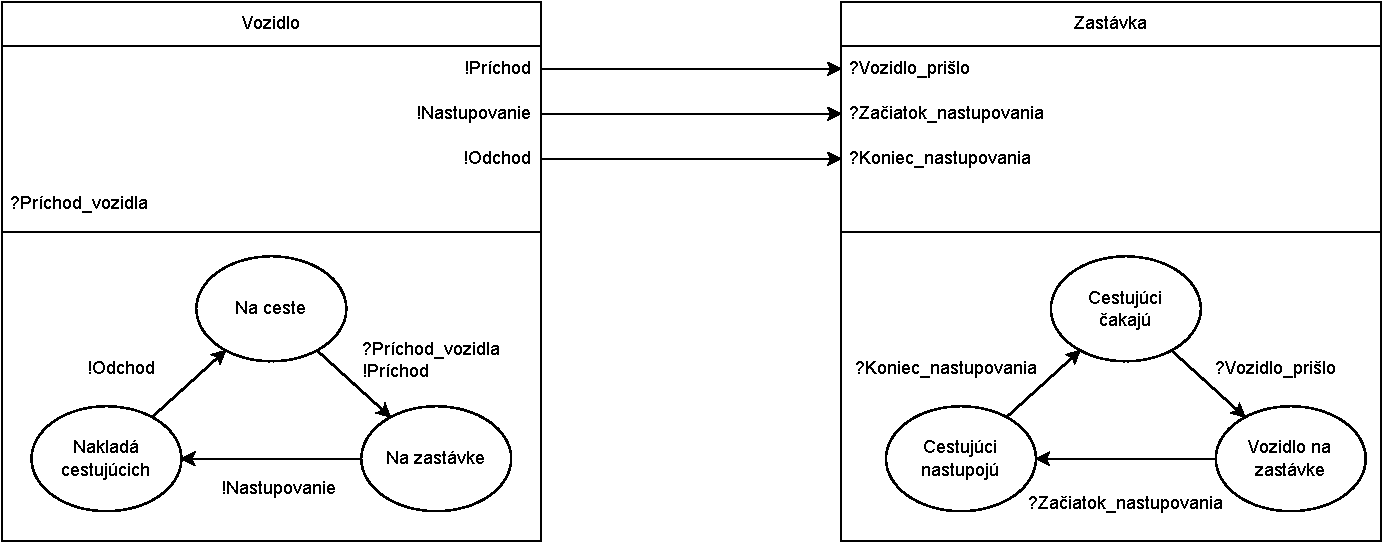
\includegraphics[width=0.9\textwidth]{DEVS-sk.drawio.pdf}
  \caption{Schéma simulačného modelu}
\end{figure}

V simulácii sa budú nachádzať viaceré inštancie modelu zastávky, každá reprezentujúc jednu zastávku na linke.
Vozidiel bude taktiež viacero, neberieme do úvahy fizcké vozidlá a fakt, že v reálnom živote sa tieto vozidlá na linke v priebehú dňa niekoľkokrát otočia.
Dôležitá je trasa, ktorú prejdu, preto jedna inštancia modelu vozidla reprezentuje jednu cestu, ktorú vozidlo prejde.
Cestujúcich v modeli nie je potrebné reprezentovať ako samostatný model, sú reprezentovaní len jedným číslom, časom kedy prišli na zastávku.
Sú súčasťou modelu zastávky, konkrétne tej na ktorej čakajú.

\subsection*{Kalendár udalostí}

Kalendár udalostí je základným prvkom modelu, ktorý riadi priebeh simulácie.
V kalendári sú uložené všetky udalosti, ktoré sa majú v modeli stať.
Tieto udalosti sú v prípade tohto modelu príchody vozidiel na zastáky.
V rámci jednej udalosti sa vykoná rutina obslúženia cestujúcich čakajúcich na zastávke.
Všetky udalosti sú naplánované na začiatku simulácie, pretože vďaka časovému rozpisu presne vieme všetky príchody vozidiel na jednotlivé zastávky.
Príchody na prvú zastávku sú dané hlavným časovým rozpisom, príchody na ostatné zastávky sú odvodené od času potrebného na prejdenie z jednej zastávky na druhú.
Pseudokód plánovania udalostí je uvedený v algoritme \ref{algoritmus_planovanie_udalosti}.
V priebehu simulácie už netreba žiadne ďalšie udalosti plánovať.

\vspace*{\dimexpr 0.5\baselineskip\relax}
\begin{algorithm}[H]
  \label{algoritmus_planovanie_udalosti}
  \caption{Plánovanie udalostí}
  \begin{algorithmic}[1]
    \FOR{čas v časovom rozpise počiatočnej zastávky}
      \STATE Vytvorí sa vozidlo
      \FOR{zastávka na linke}
        \STATE Pridá sa udalosť príchodu vozidla na danú zastávku
      \ENDFOR
    \ENDFOR
  \end{algorithmic}
\end{algorithm}
\vspace*{\dimexpr 0.5\baselineskip\relax}

Po naplánovaní všetkých udalostí sa začne simulácia.
Postupne sa vykonávajú jednotlivé udalosti a simulácia sa diskrétne posúva vpred, až kým nie je kalendár udalostí prázdny alebo nie je dosiahnutý koncový čas simulácie.
Pseudokód riadenia simulácie je popísaný v algoritme \ref{algoritmus_riadenia_simulacie}.

\vspace*{\dimexpr 0.5\baselineskip\relax}
\begin{algorithm}[H]
\label{algoritmus_riadenia_simulacie}
\caption{Simulácia riadená udalosťami}
\begin{algorithmic}[1]
  \WHILE{kalendár udalostí nie je prázdny}
    \STATE Vyberie sa udalosť s najmenším časom v kalendári
    \STATE Udalosť sa odstráni z kalendára
    \IF{čas udalosti > koncový čas simulácie}
      \STATE Simulácia končí
    \ENDIF
    \STATE Modelový čas sa nastaví na čas udalosti
    \STATE Udalosť sa vykoná
  \ENDWHILE
\end{algorithmic}
\end{algorithm}
\vspace*{\dimexpr 0.5\baselineskip\relax}

Pre potreby časového rozpisu stačí simulovať jeden deň, v prípade rôznych rozpisov v čase pracovnýh dní a v čase sviatkov a víkendov ide o kompletne iný rozpis, ktorý sa musí simulovať a optimalizovať samostatne.
Všetky naplánované udalsti by mali byť v rámci jedného dňa, preto by simulácia mala končiť vždy vyprázdnením kalendára udalostí a nie prekročením koncového času.

\subsection*{Model zastávky}
\label{model_zastavky}

Model zastávky slúži na reprezentáciu jednotlivých zastávok na linke.
Každá reálna zastávka je v systéme ako samostatná inštancia modelu zastávky.
Je pasívna, to znamená, že jej vnútorný stav sa plne odvíja od prichádzajúcich vonkajších signálov.

\begin{figure}[h]
  \label{fig:model_zastavky}
  \centering
  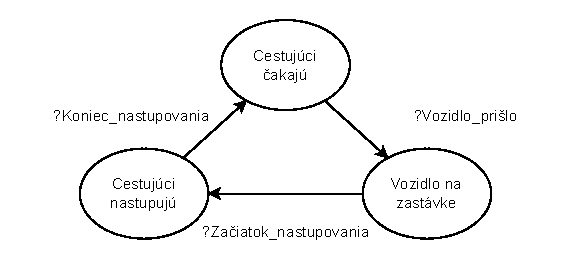
\includegraphics[width=0.6\textwidth]{DEVS-zastavka-sk.drawio.pdf}
  \caption{Stavový automat modelu zastávky}
\end{figure}

Ako je vidieť na obrázku \ref{fig:model_zastavky}, model zastávky má tri stavy:
\begin{itemize}
  \item \textbf{Cestujúci čakajú} --- na zastávke nie je žiadne vozidlo
  \item \textbf{Vozidlo na zastávke} --- na zastávku práve prišlo vozidlo
  \item \textbf{Cestujúci nastupojú} --- cestujúci nastupujú do vozidla
\end{itemize}

Dôleťitejšie sú však vstupné signály, ktorími je celý stavový automat riadený.
Zároveň sa pri prechodoch medzi stavmi vykonávajú akcie pre obsluhu cestujúcich.

Vstpný signál \textbf{?Vozidlo\_prišlo} mení vnútorný stav zastávky z \textbf{Cestujúci čakajú} na \textbf{Vozidlo na zastávke}.
Taktiež s vypočíta dĺžka intervalo medzi posledným príchodom vozidla a terajším príchodom.
Tento údaj slúži pre vygenerovanie prichádzajúcich cestujúcich.

Vstupný signál \textbf{?Začiatok\_nastupovania} mení vnútorný stav zastávky z \textbf{Vozidlo na zastávke} na \textbf{Cestujúci nastupujú}.
Pri tomto prechode sa vygenerujú časi všetkých cestujúcich, ktorí prišli od posledného príchodu vozidla.

Vstupný signál \textbf{?Koniec\_nastupovania} mení vnútorný stav zastávky z \textbf{Cestujúci nastupujú} na \textbf{Cestujúci čakajú}.
Prepíše sa čas posledného príchodu vozidla.

\subsubsection{Generovanie cestujúcich}

Cestujúci sa generujú na základne exponenciálneho rozdelenia s parametrom $\lambda$.
Tento parameter je v rámci jednej zastávky každú hodinu iný, pretože počet prichádzajúcich cestujúcich sa v priebehu dňa mení.
V algoritme \ref{algoritmus_generovanie_cestujucich} je popísaný proces generovania cestujúcich na zastávke.

\vspace*{\dimexpr 0.5\baselineskip\relax}
\begin{algorithm}[H]
\label{algoritmus_generovanie_cestujucich}
\caption{Generovanie cestujúcich}
\begin{algorithmic}[1]
  \STATE získanie $\lambda$ pre danú zastáku a hodinu
  \WHILE{modelový čas < čas príchodu autobusu}
    \STATE vygenerovanie času príchodu cestujúceho
    \STATE pridanie cestujúceho do fronty
    \STATE zmena modelového času na čas príchodu cestujúceho
  \ENDWHILE
\end{algorithmic}
\end{algorithm}

\subsection*{Model vozidla}
\label{model_vozidla}

Každé vozidlo, respektíve jedna trasa ktorú vozidlo podľa časového rozpisu prejde, je reprezentovaná jednou inštanciou modelu vozidla.
Model vozidla je na rozdiel od modelu zastávky aktívnym prvkom, nemá žiadne vstupné signály, iba výstupné.
Tieto výstupné signály sú prepojené so vstupnými signálmi modelu zastávky ako je vidieť na obrázku \ref{fig:simulacny_model}.

\begin{figure}[h]
  \label{fig:model_vozidla}
  \centering
  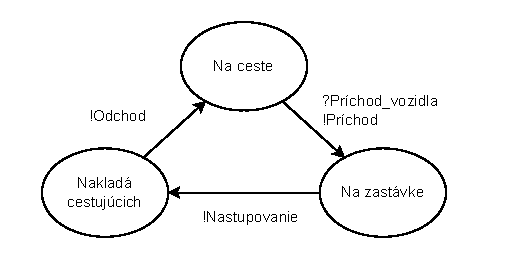
\includegraphics[width=0.6\textwidth]{DEVS-vozidlo-sk.drawio.pdf}
  \caption{Stavový automat modelu vozidla}
\end{figure}

Na obrázku \ref{fig:model_vozidla} je vidieť stavový automat modelu vozidla.
Model vozidla má tri stavy:
\begin{itemize}
  \item \textbf{Na ceste} --- vozidlo sa pohybuje medzi zastávkami
  \item \textbf{Na zastávke} --- vozidlo práve prišlo na zastávku
  \item \textbf{Nakladá cestujúcich} --- vozidlo nakladá cestujúcich
\end{itemize}

Výsupný signál \textbf{!Príchod} mení vnútorný stav vozidla z \textbf{Na ceste} na \textbf{Na zastávke}.
Pri tomto prechode vystúpia cestujúci podľa koeficientu zastávky na ktorú vozidlo práve prišlo.
Napríklad ak je vo vozidle 100 cestujúcich a koeficient zastávky je 0.7, pretože sa jedná o prestupnú zastávku, vystúpi 70 cestujúcich.

Výstupný signál \textbf{!Nastupovanie} mení vnútorný stav vozidla z \textbf{Na zastávke} na \textbf{Nakladá cestujúcich}.
Zastávka, na ktorej sa vozidlo práve nachádza tento signál zachytí a vygeneruje nových cestujúcich.
Pokiaľ to dovoluje kapacita vozidla, všetci cestujúci nastúpia.
V opačnom prípade nastúpia len tí, ktorí prišli skôr a tí čo prišli neskôr musia ostať čakať na ďalšie vozidlo.

Výstupný signál \textbf{!Odchod} mení vnútorný stav vozidla z \textbf{Nakladá cestujúcich} na \textbf{Na ceste}.
Informuje sa príslušná zastávka a nič viac sa pri tomto prechode nevykonáva.

\subsubsection{Obsluha zastávky}

Každé vozidlo začina na prvej zastávke v rozpise, ale počas simulácie sa musí pohybovať medzi zastávkami.
Proces ktorý vozidlo vykoná pri príchode na každú zastávku je popísaný v algoritme \ref{algoritmus_obsluha_zastavky}.

\vspace*{\dimexpr 0.5\baselineskip\relax}
\begin{algorithm}[H]
\label{algoritmus_obsluha_zastavky}
\caption{Obsluha zastávky}
\begin{algorithmic}[1]
  \STATE prepojenie výstupných signálov vozidla so vstupnými signálmi zastávky
  \STATE aktivácia výstupného signálu \textbf{!Príchod}
  \STATE aktivácia výstupného signálu \textbf{!Nastupovanie}
  \STATE aktivácia výstupného signálu \textbf{!Odchod}
\end{algorithmic}
\end{algorithm}

\subsection*{Udalosť príchodu vozidla na zastávku}

V rámci jednej udalosti sa vykoná rutina obslúženia cestujúcich, ktorí čakajú na zastávke. Táto rutina je popísaná v algoritme \ref{algoritmus_obsluha_zastavky}.
Parametre tejto udalosti sú:
\begin{itemize}
  \item \textbf{Čas príchodu} --- čas, kedy vozidlo prichádza na zastávku
  \item \textbf{Zastávka} --- zastávka, na ktorej sa udalosť vykonáva
  \item \textbf{Vozidlo} --- vozidlo, ktoré prichádza na zastávku
\end{itemize}

Vozidlo začína udalosť v stave \textbf{Na ceste}, príde na zastávku uvedenú v parametri udalosti, vykoná rutinu nástupu a výstupu cestujúcich a odíte na ďalšiu zastávku.
Za jednu udalosť teda vozidlo prejde všetkými svojimi vnútorným stavmi, udalosť končí v opaäť v stave \textbf{Na ceste}.
Zastávka ktorá je uvedená v parametri udalosti tiež prejde všetkými svojimi vnútornými stavmi na základe posielaných signálov od vozidla.

\section{Implementácia simulačného modelu}

Simulačný model je implementovaný v jazyku Python bez využitia externých knižníc.
Trieda \texttt{EventCalendar} obsahuje kód základných operácií nad kalendárom udalostí:
\begin{itemize}
  \item \texttt{isEmpty()} --- vráti \texttt{True} ak je kalendár udalostí prázdny, inak \texttt{False}
  \item \texttt{addEvent(event)} --- pridá udalosť do kalendára
  \item \texttt{getNextEvent()} --- vráti udalosť s najmenším časom v kalendári a odstráni ju z kalendára
\end{itemize}

Trieda \texttt{Event} reprezentuje jednu udalosť.
Obsahuje:
\begin{itemize}
  \item metóda \texttt{\_\_call\_\_()} --- vykoná akciu
  \item atribúty \texttt{action} a \texttt{actionArgument}
\end{itemize}

len metódu \texttt{\_\_call\_\_()}, ktorá vykoná udalosť uloženú v atribúte \texttt{action} s argumentami volania uloženými v \texttt{actionArgument}.

Modelový čas je implementovaný v triede \texttt{Simulation}.
Obsahuje:
\begin{itemize}
  \item metódy \texttt{forward(time)} a \texttt{getHour()}
  \item atribúty \texttt{startTime}, \texttt{currentTime} a \texttt{endTime}
\end{itemize}

Trieda \texttt{BusStop} reprezentuje jednu zastávku, rovnako tak trieda \texttt{Bus} reprezentuje jedno vozidlo.
Tieto dve triedy sú písané podľa vzoru DEVS formalizmu. Obsahujú stavy, vstupné a výstupné signály a metódy, v ktorých sa nachádzjú akcie pre jednotlivé prechody medzi stavmi.
Cestujúci sú uložení ako pole čisel, časov ich príchodu, v jednotlivých zastávkach v atribúte \texttt{waitingPassengersArrivalTimes}.

Na generovanie náhodného príchodu cestujúcich slúži trieda \texttt{RandomNumberGenerator}, ktorá obsahuje statické metódy na generovanie náhodných čísel.

Zber a agregácia štatistík (viď kapitola \ref{vystupy_simulacneho_modelu}) sú implementované v triedach \texttt{Statistics}, \texttt{BusStatistics} a \texttt{BusStopStatistics}.

Podrobnejšie informácie o kóde sa nachádzajú v programovej dokumentácii, v prílohe~\ref{prilohy_programova_dokumentacia}.
Programová dokumentácia bola vygenerovaná pomocou nástroja Sphynx.

\section{Výstupy simulačného modelu}
\label{vystupy_simulacneho_modelu}

Hlavný zmisel simulácie je zber informácií, ktoré by sme inak museli získať z pozorovania reélnej prevádzky linky.
Efektivitu každého jedného časového rozpisu, ktorý program vytvorí je potrebné otestovať a ohodnotiť aby sme našli ten najlepší z nich, skôr ako ho začneme používať v reálnej prevádzke.
Na ohodnotenie jednotlivých rozpisov slúžia štatistiky získané počas simulácie.
Štatistiky sa zbierajú pre každú zastávku aj pre každý autobus osobitne.
Následne sa agregujú do jednoho objektu \texttt{Statistics}, ktorý obsahuje:
\begin{itemize}
  \item \texttt{totalNumberOfBuses} --- počet spojov v priebehu dňa na linke
  \item \texttt{busStopStatistics} --- agregované štatistiky zastávok
  \item \texttt{busStatistics} --- agregované štatistiky vozidiel
\end{itemize}

Trieda \texttt{busStopStatistics} slúži na ukladanie informácii o jednotlivých zastávkach, ale ako bolo spomenuté vyššie tak aj na uloženie agregovaných dát.
Táto trieda slúži na zber následujúcich informácií:
\begin{itemize}
  \item \texttt{totalPassengersArrived} --- počet cestujúcich, ktorí prišli na zastávku za celý deň
  \item \texttt{totalPassengersDeparted} --- počet cestujúcich, ktorí vystúpili na zastávke za celý deň
  \item \texttt{totalPassengersLeftUnboarded} --- počet cestujúcich, ktorí museli čakať na ďalší spoj
  \item \texttt{totalTimeSpentWaiting} --- celkový čas, ktorý cestujúci strávili čakaním na zastávke
  \item \texttt{totalPassengersLeftUnboarded} --- počet cestujúcich, ktorých po celom dni nezobral žiaden spoj
  \item \texttt{passengersArrivedPerHour} --- počet cestujúcich, ktorí prišli na zastávku v jednotlivých hodinách
  \item \texttt{passengersDepartedPerHour} --- počet cestujúcich, ktorí vystúpili na zastávke v jednotlivých hodinách
  \item \texttt{passengersLeftUnboardedPerHour} --- počet cestujúcich, ktorí museli čakať na ďalší spoj v jednotlivých hodinách
  \item \texttt{timeSpentWaitingPerHour} --- čas, ktorý cestujúci strávili čakaním na zastávke v jednotlivých hodinách
\end{itemize}

Trieda \texttt{busStatistics} má rovnaký účel ako trieda \texttt{busStopStatistics}, ale pre vozidlá.
Zbiera informácie:
\begin{itemize}
  \item \texttt{capacity} --- kapacita vozidla
  \item \texttt{averageLoad} --- priemerná naplnenosť vozidla
  \item \texttt{averageLoadInPercent} --- priemerná naplnenosť vozidla v percentách
  \item \texttt{totalPassengersTransported} --- celkový počet prevezených cestujúcich
  \item \texttt{loadPerBusStop} --- naplnenosť vozidla na jednotlivých zastávkach
  \item \texttt{loadInPercentPerBusStop} --- naplnenosť vozidla na jednotlivých zastávkach v percentách
\end{itemize}

\subsection*{Počet spojov v priebehu dňa na linke}
Tento údaj slúži pre optimalizáciu, z pohľadu dopravného podniku chceme, aby bol pocet spojov čo najmenší aby ušetrili na prevádzkových nákladoch.
Z pohľadu cestujúcich chceme aby bol počet spojov čo najväčší, aby nemuseli čakať na spoj dlhšie ako je nutné.
Je potrebné nájsť kompromis medzi týmito dvoma extrémami.

\subsection*{Počet cestujúcich, ktorí prišli na zastávku za celý deň}
Celkový počet cestujúcich za deň je dobrím indikátorom toho, ako sú namáhané jednotlivé časti linky.
V prípadoch, kedy na zastávky v strede trasy prichádza oveľa viac cestujúcich ako na koncové zastávky, posilňuje dopravný podnik práve túto strednú časť ďalšími spojmi.
Tieto spoje však na koncové zastávky už nechodia.

\subsection*{Počet cestujúcich, ktorí vystúpili na zastávke za celý deň}
Je potrebné aby sme v rámci simulácie rátali aj s cestujúcimi, ktorí z vozidiel vystupujú, inak by sa kapacita vozidla hneď naplnila.
Ide o dôležitú časť reálneho systému, ktorú nemôžeme zanedbať ani pri simulácii.
Slúži na validáciu modelu.

\subsection*{Počet cestujúcich, ktorí museli čakať na ďalší spoj}
Občas sa stane, že je vozidlo tak preplnené, že nie všetci cestujúci, ktorí čakali na zastávke do neho nastúpia.
V reálnom živote ide asi o subjektívny pocit, či nastúpiť alebo nie.
V simulačnom modeli cestujúci prestanú nastupovať v momente keď naplnenosť vozidla dosiahne jeho maximálnu kapacitu.
Rozpisy, pri ktorých sa tento jav vyskytne budú mať horšie hodnotenie.

\subsection*{Celkový čas, ktorý cestujúci strávili čakaním na zastávke}
Z pohľadu optimalizácie chceme, aby bol tento čas čo najnižší.
Príliš dlhé čakanie na zastávke bude rozpisy ohodnocovať negatívne.
V prípade, že cestujúci musel čakať na ďalší spoj, tento šas bude ešte dlhší.
Treba rátať aj s cestujúcimi, ktorí na zastávku prídu tesne pred odchodom vozidla.
Napríklad ak chodí spoj dvakrát za hodinu, je oveľa vyššia pravdepodobnosť, že cestujúci nepríde v náhodný čas, ale svoj príchod na zastávku si naplánuje.

\subsection*{Počet cestujúcich, ktorých po celom dni nezobral žiaden spoj}
Podobne ako v prípade cestujúcich, ktorí museli čakať na ďalší spoj, aj týchto cestujúcich by sme mali rátať a rozpis by mal byť ohodnotený veľmi negatívne.
Tento jav by mohol v reálnom svete nastať asi iba ak by cestujúci išiel na posledný spoj v dni a toto vozidlo by bolo úplne preplnené.
Ale keďže optimalizácia v tomto programe je riešená genetickým algoritmom, je veľká šanca že sa tento jav vyskytne častejšie.
Táto vlastnosť je nežiaduca a je potrebné ju eliminovať.

\subsection*{Počet cestujúcich, ktorí prišli na zastávku v jednotlivých hodinách}
Tento údaj má skôr informatívny charakter, pretože ide o vstup programu.
Algoritmus sa snaží vytvoriť rozpis, ktorý by bol schopný prepraviť všetkých cestujúcich.
Na grafe \ref{fig:passengersArrivedPerHour} je vidieť, že v priebehu dňa sa počet cestujúcich prichádzajúcich na zastávku mení.
Obzvlášť v ranných a poobedných hodinách je tento počet výrazne vyšší ako počas dňa.
V týchto časoch by malo chodiť viac spojov.
\begin{figure}[h]
  \label{fig:passengersArrivedPerHour}
  \centering
  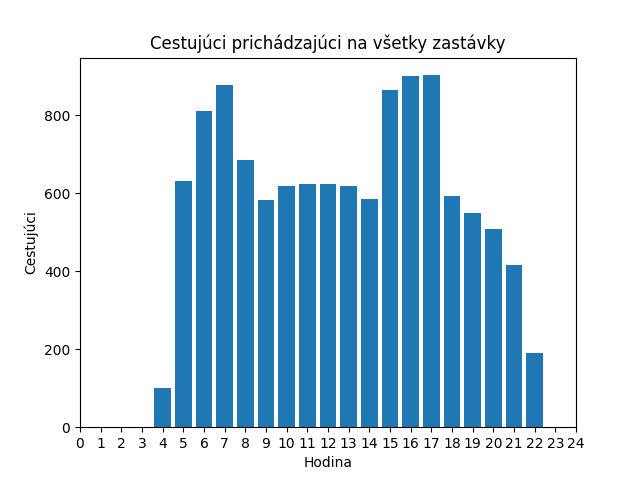
\includegraphics[width=0.5\textwidth]{passengersArrivedPerHour.png}
  \caption{Počet cestujúcich, ktorí prišli na zastávku v jednotlivých hodinách}
\end{figure}

\subsection*{Počet cestujúcich, ktorí vystúpili na zastávke v jednotlivých hodinách}
Ide o rovnaký údaj ako bol počet cestujúcich, ktorí vystúpili na zastávke za celý deň, ale rozdelený na jednotlivé hodiny dňa.
Je vidieť, že graf \ref{fig:passengersDepartedPerHour} má podobný tvar ako graf \ref{fig:passengersArrivedPerHour}.
To je správne, pretože počet cestujúcich, ktorí vystúpili na zastávke by mal byť rovnaký ako počet cestujúcich, ktorí prišli na zastávku.
Mohlo by sa stať, že tieto dve hodnoty by sa líšili, v prípade, že ostatnú cestujúci, ktorí sa v priebehu dňa nezmestili do žiadneho vozidla.
\begin{figure}[h]
  \label{fig:passengersDepartedPerHour}
  \centering
  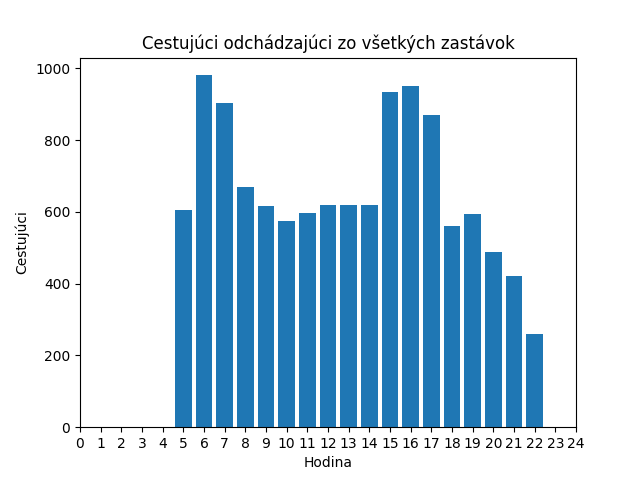
\includegraphics[width=0.5\textwidth]{passengersDepartedPerHour.png}
  \caption{Počet cestujúcich, ktorí vystúpili na zastávke v jednotlivých hodinách}
\end{figure}

\subsection*{Počet cestujúcich, ktorí museli čakať na ďalší spoj v jednotlivých hodinách}
Na ľavej strane grafu \ref{fig:passengersLeftUnboardedPerHour} je vidieť, že v priebehu ďňa žiaden z cestujúcich nemusel čakať na ďalší spoj.
Toto je ideálny stav.
Na pravej strane grafu \ref{fig:passengersLeftUnboardedPerHour} je vidieť, že v priebehu dňa sa počet cestujúcich, ktorí museli čakať na ďalší spoj mení.
Ráno a okolo obeda nemusel na ďalší spoj čakať nikto, ale v poobednej špičke je vidieť zjavný nedostatok spojov, pretože cestujúci musia čakať na ďalší spoj.
\begin{figure}[h]
  \label{fig:passengersLeftUnboardedPerHour}
  \centering
  \begin{minipage}{0.49\textwidth}
    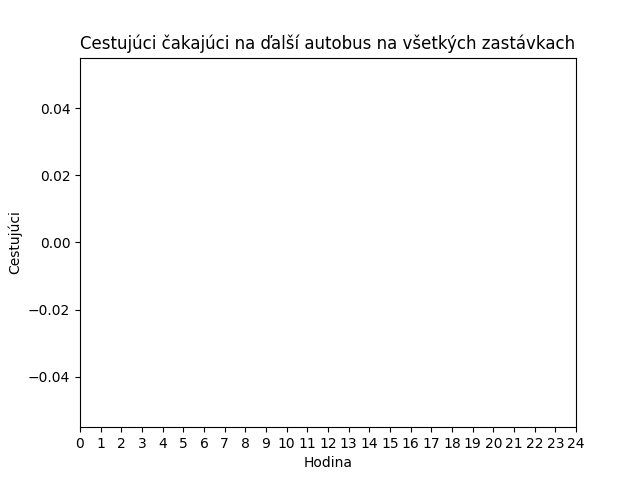
\includegraphics[width=\textwidth]{passengersLeftUnboardedPerHour.png}
  \end{minipage}
  \begin{minipage}{0.49\textwidth}
    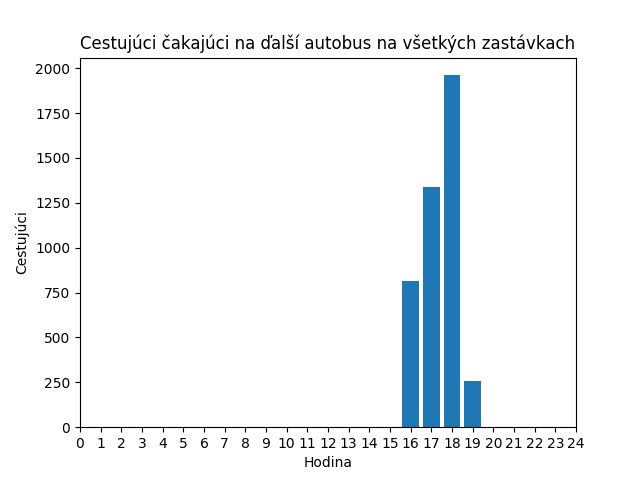
\includegraphics[width=\textwidth]{passengersLeftUnboardedPerHour_nonoptimal.png}
  \end{minipage}
  \caption{Počet cestujúcich, ktorí museli čakať na ďalší spoj v jednotlivých hodinách}
\end{figure}

\subsection*{Čas, ktorý cestujúci strávili čakaním na zastávke v jednotlivých hodinách}
Čas strávený čakaním na zastávke by mal byť počas celého dňa približne rovnaký.
Na ľavej strane grafu \ref{fig:timeSpentWaitingPerHour} je tento optimálny stav vidieť.
Bez ohľadu na to, kedy cestujúci prídu na zastávku, čakajú na spoj rovnako dlho.
Naopak na prave strane grafu \ref{fig:timeSpentWaitingPerHour}, ktorý je výstupom rovnakej simulácie ako pravá strana grafu \ref{fig:passengersLeftUnboardedPerHour}, je zrejmé, že čas čakania na zastávke sa v poobedných hodinách výrazne zvýšil práve kvoli tomu, že cestujúci museli čakať na ďalší spoj.
\begin{figure}[h]
  \label{fig:timeSpentWaitingPerHour}
  \centering
  \begin{minipage}{0.49\textwidth}
    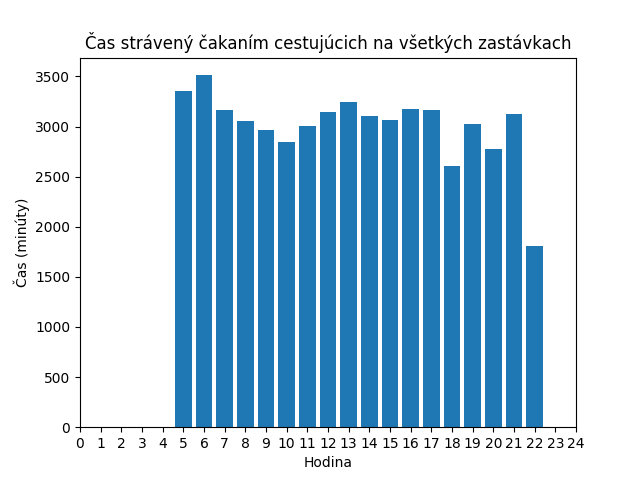
\includegraphics[width=\textwidth]{timeSpentWaitingPerHour.png}
  \end{minipage}
  \begin{minipage}{0.49\textwidth}
    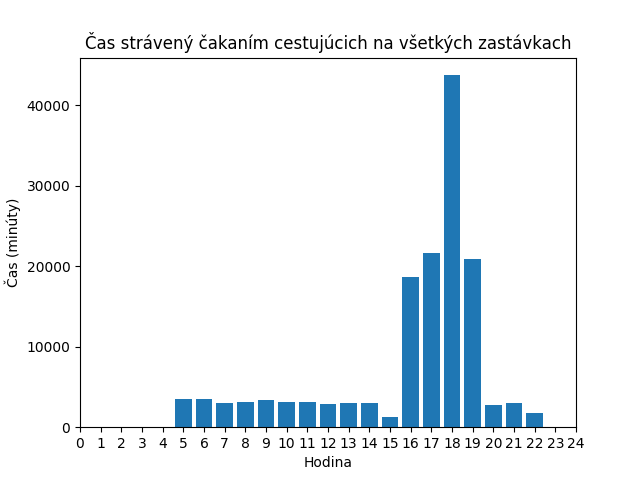
\includegraphics[width=\textwidth]{timeSpentWaitingPerHour_nonoptimal.png}
  \end{minipage}
  \caption{Čas, ktorý cestujúci strávili čakaním na zastávke v jednotlivých hodinách}
\end{figure}

\subsection*{Kapacita vozidla}
Tento parameter je dôležitý, pretože na základe neho sa rozhoduje, koľko cestujúcich môže nastúpiť do vozidla.
Zároveň slúži pre výpočet naplnenosti vozidla v percentách.
Príliš malá alebo príliš veľká naplnenosť vozidla môže byť nežiaduca.
Na ohodnotenie toho, ako moc je vozidlo naplnené teda treba poznať aj jeho kapacitu.

\subsection*{Priemerná naplnenosť vozidla}
Priemerná naplnenosť vozidla je dôležitý parameter, ktorý nám hovorí, ako moc sú vozidlá využívané.
Z pohľadu cestujúcich je lepšie, ak je vozidlo prázdnejšie, ale z pohľadu dopravného podniku je to nevyužitý potenciál.
Preto je potrebné nájsť kompromis medzi týmito dvoma požiadavkami.
To aká naplnenosť je optimálna je už úlohou analytika, ktorý bude tento program využívať.
Povedzme, že sa rozhodne pre naplnenosť 70\%.
Potom čim ďalej bude priemerná naplnenosť vozidiel od tejto hodnoty, tým horšie bude rozpis ohodnotený.

\subsection*{Celkový počet prevezených cestujúcich}
Celkový počet prevezených cestujúcich záleží od toho, koľko cestujúcich prišlo na jednotlivé zastávky a či sa im podarilo nastúpiť do vozidiel.
V ideálnom prípade sa tento počet bude rovnať počtu cestujúcich, ktorí prišli na zastávky.
V extrémnych prípadoch sa môže stať, že niektorí cestujúci zostanú na zastávkach a nezoberie ich žiadne vozidlo.
V prípade štatistiky jednotlivých vozidiel, môže byť tento počet použitý na ich porovnanie.
Počas dňa by mali všetky vozidlá prepraviť približne rovnaký počet cestujúcich.
Ak tomu tak nie je a sú vyťažené nerovnomerne, rozpis by sa mal ohodnotiť negatívne.

\subsection*{Naplnenosť vozidla na jednotlivých zastávkach}
Na grafe \ref{fig:averageLoad} je znázornené ako sa naplnenosť vozidiel mení počas ich jazdy.
Konkrétne sa jedná o linku 46 v Brne.
Naplnenosť sa postupne zvyšuje až kým nepríde na jednu z hlavných prestupných zastávok, Štefánikova čtvrť.
Tu vystúpi veľké množstvo cestujúcich a naplnenosť vozidla sa zníži.
Pokiaľ má linka príliš veľké výkivy v naplnenosti vozidiel naprieč svojou trasou, môže to byť znakom toho, že je potrebné trasu na určitých úsekoch posilniť inou linkou.
\begin{figure}[h]
  \label{fig:averageLoad}
  \centering
  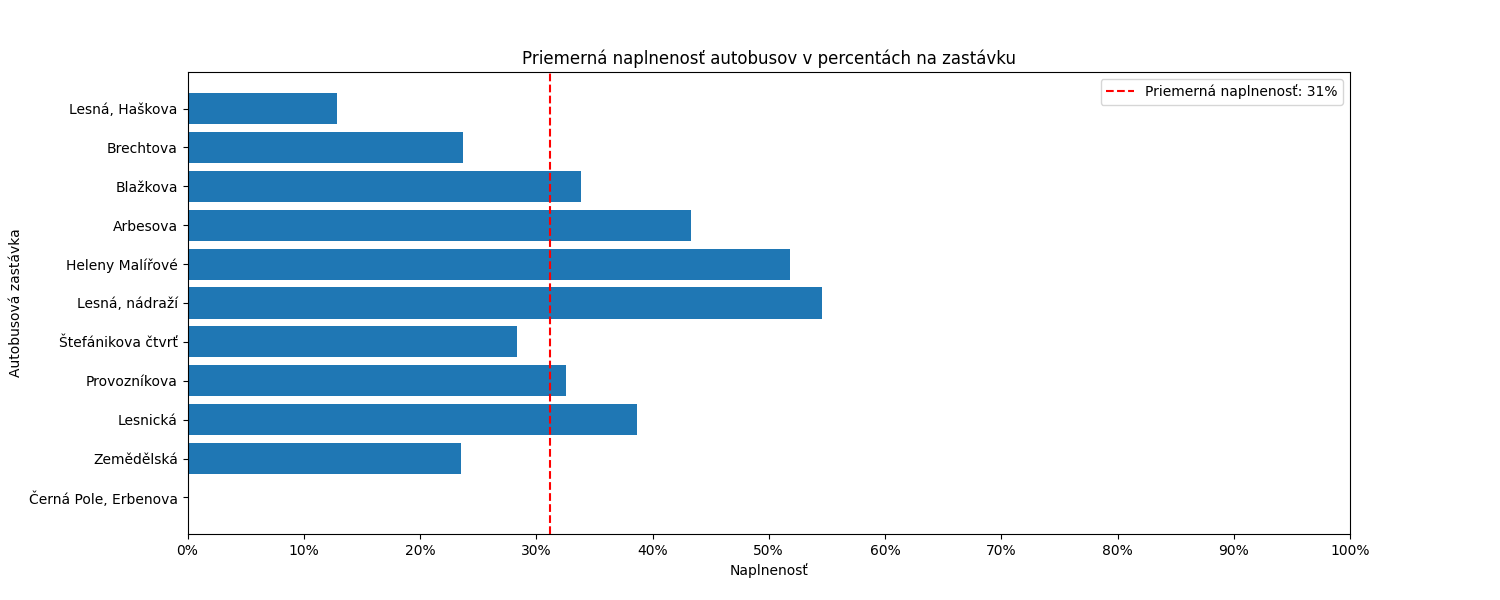
\includegraphics[width=\textwidth]{loadInPercentPerBusStop.png}
  \caption{Priemerná naplnenosť vozidla na jednotlivých zastávkach}
\end{figure}





































\chapter{Optimalizácia časového rozpisu linky mestskej hormadnej dopravy} % 15 strán
\label{optimalizacia}

Optimalizácia časového rozpisu je zložitý problém s veľkým množstvom premenných a obmedzení.
Táto kapitola pojednáva o daných vstupoch, obmedzeniach, použitej optimalizačnej metóde a výstupoch optimalizácie.

Na optimalizáciu bol použitý genetický algoritmus.
Genetický algoritmus je heuristická optimalizačná metóda, ktorá sa inšpiruje evolučnou biológiou.
Je založená na princípe prírodného výberu, kde sa najlepšie jedince z populácie vyberajú na reprodukciu a vytvárajú novú generáciu.
Tento proces sa opakuje, až kým sa nenájde optimálne riešenie alebo sa nedosiahne maximálny počet generácií.
Na ohodnotenie jedinca sa používa fitness funkcia, ktorá hodnotí kvalitu riešenia na základe zadaných kritérií.
V prípade časových rozpisov MHD sa na výpočet fitness funkcie používajú štatistiky zo simulácie, ktoré sú popísané v kapitole \ref{vystupy_simulacneho_modelu}.

\section{Vstupy potrebné od používateľa}
Na to aby mohol algoritmus fungovať, je potrebné zadať niekoľko vstupných parametrov.
Najdôležitejším z nich sú informácie o zastávkach. O každej zastávke je potrebné zadať:
\begin{itemize}
  \item \textbf{Názov zastávky} --- názov zastávky, ktorý sa zobrazuje na výstupoch
  \item \textbf{Čas príchodu} --- čas potrebný na prejdenie vzdialenosti od prvej zastávky po túto zastávku
  \item \textbf{Štatistika o príchodoch cestujúcich} --- priemerný počet prichádzajúcich cestujúcich v každej hodine dňa
  \item \textbf{Pravdepodobnosť výstupu cestujúceho} --- údaj potrebný pre priebežné vyprázdnenie vozidla
\end{itemize}
Ďalšie dôležité informácie o linke sú:
\begin{itemize}
  \item \textbf{Kapacita vozidla} --- maximálny počet cestujúcich, ktorý sa zmestí do vozidla
  \item \textbf{Miest na sedenie} --- počet miest na sedenie v vozidle
  \item \textbf{Celkové náklady} --- udávané v Kč/100 miesto-km (tabuľková hodnota) 
  \item \textbf{Dĺžka trasy} --- dĺžka trasy v km
\end{itemize}
Potom je potrebné zadať parametre genetického algoritmu:
\begin{itemize}
  \item \textbf{Veľkosť populácie} --- počet jedincov v jednej generácii
  \item \textbf{Počet generácií} --- počet generácií, ktoré sa majú vykonať
  \item \textbf{Pravdepodobnosť mutácie} --- pravdepodobnosť, že sa v jedincovi vyskytne mutácia
  \item \textbf{Maximálny počet spojov za hodinu} --- maximálny počet spojov, ktorý môže byť vygenerovaný za hodinu
\end{itemize}
Poslednou informáciou, ktorá je od používateľa potrebná sú obmedzenia na počet spojov za hodinu.
Používateľ takto môže nastaviť fixný počet spojov, ktorý sa má vygenerovať za hodinu.
Toto sa využíva hľavne pri plánovaní náväznosti liniek, kedy je potrebné aby sa niektoré spoje stretli na prestupnej zastávke.
Obvykle sa to robí tak, že sa nastaví rovnaký počet spojov pre všetky prestupné linky, ktoré sa na tejto zastávke stretávajú.
Toto obmedzenie využíva aj predbežná analýza, ktorá sa vykonáva pred optimalizáciou.
V prípade ak pre niektorú hodinu neexistuje údaj o priemernom počte prichádzajúcich cestujúcich naprieč všetkými zastávkami, nastaví sa fixný počet spojov v danej hodine na 0.
Tento krok výrazne prispieva k lepším výsledkom optimalizácie, pretože dopredu vieme, že v tejto hodine nebude žiaden spoj potrebný.
Zároveň s nižším počtom spojov vo všetkých rozpisoch počas optimalizácie sa výpočet výrazne urýchli.

\section{Implementácia genetického algoritmu}


\section{Výstupy optimalizácie}

















































\chapter{Experimenty} % 10 strán
\label{experimenty}

V tejto kapitole sú podrobne popísané experimentálne scenáre, ktoré boli navrhnuté na posúdenie výkonnosti optimalizačného algoritmu aplikovaného na plánovanie liniek MHD.
Cieľom bolo preskúmať, ako algoritmus reaguje na zmeny v parametroch ako sú dĺžka trasy, dĺžka vozidla a počet zastávok.

Každý experiment bol vykonaný s rovnakými parametrami pre genetický algoritmus, aby sa zabezpečila konzistentnosť výsledkov:
\begin{itemize}
  \item \textbf{Počet jedincov v populácii} --- 50 pre krátku trasu, 10 pre dlhú trasu \footnote{Tento počet bol znížený z dôvodu dlhšej doby výpočtu.}
  \item \textbf{Počet generácií} --- 100
  \item \textbf{Pravdepodobnosť mutácie} --- 5\%
  \item \textbf{Maximálny počet spojov za hodinu} --- 15
\end{itemize}
Ostatné parametre sú špecifické pre jednotlivé experimenty a sú uvedené v tabuľkách v príslušných sekciách.

Parametre zariadenia na ktorom boli experimenty vykonané sú:
\begin{itemize}
  \item \textbf{Operačný systém} --- Windows 11 Pro 64-bit
  \item \textbf{Procesor} --- Intel Core i7-9750H CPU @ 2.60GHz
  \item \textbf{RAM} --- 16 GB DDR4
\end{itemize}

Všetky experimenty boli vykonané na rovnakom zariadení, aby sa zabezpečila konzistentnosť výsledkov,
a v rovnakom čase, aby sa minimalizoval vplyv vonkajších faktorov.
Každý experiment trval približne od 45 minút do 1.5 hodiny v závislosti od dĺžky trasy a počtu zastávok.

\newpage
\section{Experiment s krátkou trasou a krátkym vozidlom}
Cieľom tohto experimentu je zistiť, ako sa algoritmus vyrovnáva s krátkou trasou a krátkym vozidlom.
Ako referencia bola zvolená linka 46 v Brne, ktorej trasa pozostáva z 11 zastávok.
Parametry experimentu sú uvedené v tabuľke \ref{tab:shortDshortVin}.

\begin{table}[h]
  \centering
  \begin{tabular}{|l|c|}
    \hline
    \textbf{Vstup} & \textbf{Hodnota} \\ \hline
    Kapacita vozidla & 80 \\ \hline
    Miest na sedenie & 30 \\ \hline
    Celkové náklady & 92,82 Kč/100 miesto-km \\ \hline
    Dĺžka trasy & 3,8 km \\ \hline
  \end{tabular}
  \caption{Parametre vozidla a trasy}
  \label{tab:shortDshortVin}
\end{table}

Ako je vidieť v tabuľke \ref{tab:shortDshortVout}, optimalizácia prebehla úspešne.
Algoritmus bol schopný vygenerovať rozpis, pri ktorom je spokojnosť cestujúcich 94\% a počet cestujúcich.
Vozidlá sú v priemere zaplnené do jednej tretiny, pretože ich je až 115, to je o 3 spoje menej ako je aktu8lny rozpis linky 46.

\begin{table}[h]
  \centering
  \begin{tabular}{|l|c|}
    \hline
      \textbf{Výstup} & \textbf{Hodnota} \\ \hline
      Počet príchodov cestujúcich & 11603 \\ \hline
      Počet prevezených cestujúcich & 11603 \\ \hline
      Počet neobslúžených cestujúcich & 0 (0,0\,\%) \\ \hline
      Celkový čas strávený čakaním & 54625 min \\ \hline
      Priemerný čas strávený čakaním & 5 min \\ \hline
      Celkové náklady & 32450 Kč \\ \hline
      Priemerná spokojnosť cestujúcich & 94,0\,\% \\ \hline
      Celkový počet vozidiel & 115 \\ \hline
      Priemerná naplnenosť vozidiel & 25 (31,02\,\%) \\ \hline
  \end{tabular}
  \caption{Výstupy simulácie}
  \label{tab:shortDshortVout}
\end{table}

Celý rozpis zastávok, časový rozpis a grafy podrobnejšie popisujúce tento experiment sú uvedené v prílohe \ref{shortDshortV}.

\newpage

\section{Experiment s krátkou trasou a dlhým vozidlom}
Cieľom tohto experimentu je zistiť, ako sa algoritmus vyrovnáva s krátkou trasou a dlhým vozidlom.
Ako referencia bola zvolená linka 46 v Brne, ktorej trasa pozostáva z 11 zastávok.
Parametry experimentu sú uvedené v tabuľke \ref{tab:shortDlongVin}.

\begin{table}[h]
  \centering
  \begin{tabular}{|l|c|}
    \hline
    \textbf{Vstup} & \textbf{Hodnota} \\ \hline
    Kapacita vozidla & 160 \\ \hline
    Počet miest na sedenie & 60 \\ \hline
    Celkové náklady & 92,82 Kč/100 miesto-km \\ \hline
    Dĺžka trasy & 3,8 km \\ \hline
  \end{tabular}
  \caption{Parametre vozidla a trasy}
  \label{tab:shortDlongVin}
\end{table}

V tabuľke \ref{tab:shortDlongVout} sú vidieť zmeny oproti predošlému experimentu.
Navýšenie kapacity jednoho vozidla má vplyv na:
\begin{itemize}
  \item Priemerná čakacia doba sa zvýšila o 2 minúty
  \item Spokojnosť cestiujúcich sa zvýšila o 4,54\%
  \item Počet vozidiel sa znížil o 43 kusov
  \item Priemerná naplnenosť vozidiel sa znížila o 6,42\%
\end{itemize}

\begin{table}[h]
  \centering
  \begin{tabular}{|l|c|}
    \hline
      \textbf{Výstup} & \textbf{Hodnota} \\ \hline
      Počet príchodov cestujúcich & 11528 \\ \hline
      Počet prevezených cestujúcich & 11528 \\ \hline
      Počet neobslúžených cestujúcich & 0 (0,0\,\%) \\ \hline
      Celkový čas strávený čakaním & 86013 min \\ \hline
      Priemerný čas strávený čakaním & 7 min \\ \hline
      Celkové náklady & 40633 Kč \\ \hline
      Priemerná spokojnosť cestujúcich & 98,54\,\% \\ \hline
      Celkový počet vozidiel & 72 \\ \hline
      Priemerná naplnenosť vozidiel & 39 (24,6\,\%) \\ \hline
  \end{tabular}
  \caption{Výstupy simulácie}
  \label{tab:shortDlongVout}
\end{table}

Celý rozpis zastávok, časový rozpis a grafy podrobnejšie popisujúce tento experiment sú uvedené v prílohe \ref{shortDlongV}.

\newpage

\section{Experiment s dlhou trasou a krátkym vozidlom}
Cieľom tohto experimentu je zistiť, ako sa algoritmus vyrovnáva s dlhou trasou a krátkym vozidlom.
Ako referencia bola zvolená okružná linka 84 v Brne, ktorej trasa pozostáva zo 44 zastávok.
Parametry experimentu sú uvedené v tabuľke \ref{tab:longDshortVin}.

\begin{table}[h]
  \centering
  \begin{tabular}{|l|c|}
    \hline
    \textbf{Vstup} & \textbf{Hodnota} \\ \hline
    Kapacita vozidla & 80 \\ \hline
    Počet miest na sedenie & 30 \\ \hline
    Celkové náklady & 92,82 Kč/100 miesto-km \\ \hline
    Dĺžka trasy & 23,0 km \\ \hline
  \end{tabular}
  \caption{Parametre vozidla a trasy}
  \label{tab:longDshortVin}
\end{table}

Z tabuľky \ref{tab:longDshortVout} je vidieť, že algoritmus bol schopný vygenerovať rozpis, pri ktorom je spokojnosť cestujúcich viac ako 98\%.
Priemerná čakacia doba, počet vozidiel a priemerná naplnenosť vozidiel sú veľmi podobné ako v prípade krátkej trasy.
Oproti nej však vzrástol počet cestujúcich a teda aj celkový čas strávený čakaním.
Taktiež sa zvýšili celkové náklady na prevádzku.

\begin{table}[h]
  \centering
  \begin{tabular}{|l|c|}
    \hline
      \textbf{Výstup} & \textbf{Hodnota} \\ \hline
        Počet príchodov cestujúcich & 49041 \\ \hline
        Počet prevezených cestujúcich & 49041 \\ \hline
        Počet neobslúžených cestujúcich & 0 (0,0\,\%) \\ \hline
        Celkový čas strávený čakaním & 253052 min \\ \hline
        Priemerný čas strávený čakaním & 5 min \\ \hline
        Celkové náklady & 189576 Kč \\ \hline
        Priemerná spokojnosť cestujúcich & 98,1\,\% \\ \hline
        Celkový počet vozidiel & 111 \\ \hline
        Priemerná naplnenosť vozidiel & 22 (27,67\,\%) \\ \hline
  \end{tabular}
  \caption{Výstupy simulácie}
  \label{tab:longDshortVout}
\end{table}

Celý rozpis zastávok, časový rozpis a grafy podrobnejšie popisujúce tento experiment sú uvedené v prílohe \ref{longDshortV}.

\newpage
\section{Experiment s dlhou trasou a dlhým vozidlom}
Cieľom tohto experimentu je zistiť, ako sa algoritmus vyrovnáva s dlhou trasou a dlhým vozidlom.
Ako referencia bola zvolená okružná linka 84 v Brne, ktorej trasa pozostáva zo 44 zastávok.
Parametry experimentu sú uvedené v tabuľke \ref{tab:longDlongVin}.

\begin{table}[h]
  \centering
  \begin{tabular}{|l|c|}
    \hline
    \textbf{Vstup} & \textbf{Hodnota} \\ \hline
    Kapacita vozidla & 160 \\ \hline
    Počet miest na sedenie & 60 \\ \hline
    Celkové náklady & 92,82 Kč/100 miesto-km \\ \hline
    Dĺžka trasy & 23,0 km \\ \hline
  \end{tabular}
  \caption{Parametre vozidla a trasy}
  \label{tab:longDlongVin}
\end{table}

Výstupy experimentu je možné vidieť v tabuľke \ref{tab:longDlongVout}.
Oproti experimentu s dlhou cestou ale krátkym vozidlom sa zmenili následovné parametre:
\begin{itemize}
  \item Priemerná čakacia doba sa zvýšila o 2 minúty
  \item Spokojnosť cestiujúcich sa zvýšila o 1,88\%
  \item Počet vozidiel sa znížil o 29 kusov
  \item Priemerná naplnenosť vozidiel sa znížila o 9,04\%
\end{itemize}

\begin{table}[h]
  \centering
  \begin{tabular}{|l|c|}
    \hline
      \textbf{Výstup} & \textbf{Hodnota} \\ \hline
        Počet príchodov cestujúcich & 48358 \\ \hline
          Počet prevezených cestujúcich & 48358 \\ \hline
          Počet neobslúžených cestujúcich & 0 (0,0\,\%) \\ \hline
          Celkový čas strávený čakaním & 314379 min \\ \hline
          Priemerný čas strávený čakaním & 7 min \\ \hline
          Celkové náklady & 280094 Kč \\ \hline
          Priemerná spokojnosť cestujúcich & 99,98\,\% \\ \hline
          Celkový počet vozidiel & 82 \\ \hline
          Priemerná naplnenosť vozidiel & 30 (18,63\,\%) \\ \hline
  \end{tabular}
  \caption{Výstupy simulácie}
  \label{tab:longDlongVout}
\end{table}

Celý rozpis zastávok, časový rozpis a grafy podrobnejšie popisujúce tento experiment sú uvedené v prílohe \ref{longDlongV}.

\chapter{Záver} % 1 strana
\label{zaver}
































% % Tento soubor nahraďte vlastním souborem s obsahem práce.
% %=========================================================================
% % Autoři: Michal Bidlo, Bohuslav Křena, Jaroslav Dytrych, Petr Veigend a Adam Herout 2019

% % Pro kompilaci po částech (viz projekt.tex), nutno odkomentovat a upravit
% %\documentclass[../projekt.tex]{subfiles}
% %\begin{document}

% \chapter{Úvod}

% Tento text slouží jako ukázkový obsah šablony a současně rekapituluje nejdůležitější informace z předpisů a poskytuje další užitečné informace, které budete potřebovat pro tvorbu technické zprávy ke svojí práci. Než se šablonou budete dále pracovat, je třeba vědět, jak ji správně použít. To je stručně uvedeno v~příloze \ref{jak}.

% I když některým studentům pro napsání dobré diplomové práce (bakalářská práce je také diplomová -- dostává se za ni diplom) stačí znát a dodržovat oficiální formální požadavky uvedené ve směrnicích a typografické zásady, často je výhodné před započetím psaní zjistit, jaké jsou osvědčené postupy pro psaní odborného textu a jak si práci usnadnit. Někteří vedoucí svým studentům připravili popisy osvědčených postupů, které vedly k desítkám úspěšně obhájených prací. Výběr nejzajímavějších postupů, které měli autoři této šablony k~dispozici ve chvíli její tvorby, je v níže uvedených kapitolách. Má-li Váš vedoucí svoji stránku s doporučenými postupy, tyto kapitoly můžete vynechat a řídit se pokyny svého vedoucího. Pokud takovou stránku nemá, může být přečtení níže uvedeného textu vhodnou přípravou na konzultaci o plánované struktuře a náplni textu práce.

% Diplomová práce je rozsáhlé dílo a tomu odpovídá i technická zpráva. Ne každý je schopen si sednout a jednoduše ji napsat. Je třeba vědět, kde začít a jak postupovat. Jedním z možných přístupů je začít psaním klíčových slov a abstraktu, abyste si ujasnili, co je v~práci nejdůležitější. O tom pojednává kapitola \ref{abstrakt}.

% Po sepsání abstraktu se lze pustit do psaní samotného textu technické zprávy. Typicky si nejprve připravíme základní strukturu práce, kterou pak budeme plnit textem. Kapitola \ref{struktura} se zabývá základními informacemi a radami pro psaní odborného textu, které Vám pomohou vyhnout se začátečnickým chybám, a stanovením nadpisů kapitol a přibližných rozsahů jednotlivých částí práce. V závěru kapitoly je pak uveden přístup, kterým si lze psaní technické zprávy značně usnadnit.

% Diplomové práce v oblasti informačních technologií mají určitou typickou strukturu. Po~úvodu bude následovat kapitola či kapitoly zabývající se shrnutím současného stavu, který bude v následujících kapitolách zhodnocen a bude navrženo řešení, které bude implementováno a otestováno. V závěru pak budou výsledky vyhodnoceny a bude navržen budoucí vývoj. I když se názvy a rozsahy kapitol v různých pracích liší, vždy tam lze najít kapitoly odpovídající této struktuře. Kapitola \ref{kapitoly} se zabývá obsahy typických kapitol, které se v diplomových pracích z oblasti IT vyskytují. Většina studentů ve svojí práci pravděpodobně využije pouze určitou podmnožinu popsaných kapitol, která je pro jejich práci relevantní. Uvedené popisy a rady mohou pomoci jak s~rozhodnutím, zda danou kapitolu uvést, tak i~s~vnitřní strukturou a samotným obsahem kapitoly.

% Za závěrečnou kapitolou práce vždy následuje seznam použité literatury. Citacemi, které tento seznam tvoří, a odkazy na ně se zabývá kapitola \ref{citace}. Byť to tak nezkušený student nemusí vnímat, je seznam použité literatury a odkazy na něj pro práci zcela zásadní. Hodnocení práce s literaturou a citací tvoří jednu z důležitých částí posudku oponenta a bude-li chybět jediná položka, může to vést k hodnocení stupněm F, následnému disciplinárnímu řízení za plagiátorství a k vyloučení z nedokončeného studia. Nesprávná práce se zdroji může mít i další důsledky -- v roce 2018 stála křesla dva členy české vlády. Proto prosím citacím věnujte odpovídající pozornost. 

% Po dokončení textu je nutné zjistit, jaké požadavky jsou kladeny na vysokoškolskou kvalifikační práci na FIT VUT v~Brně, a dořešit případné nedostatky. Formální požadavky jsou uvedeny ve směrnicích a na webových stránkách, které jsou zmíněny v kapitole \ref{formality}. Tato kapitola obsahuje i požadované rozsahy jednotlivých typů prací a další vybrané informace z~předpisů a doporučení. V závěru kapitoly je uveden přehled nejčastějších chyb, se kterými se oponenti setkávají a kterým byste se měli vyhnout. Hodnocení formální úpravy práce je pak další z důležitých součástí posudku oponenta.

% Po odstranění formálních nedostatků lze práci odevzdat. Před odevzdáním práce si můžete projít kontrolní seznam (tzv. \uv{checklist}) uvedený v příloze \ref{checklist}. Samotné odevzdání listinné i elektronické verze práce je pak popsáno v kapitole \ref{odevzdani}.

% V závěrečné kapitole \ref{zaver} je pak uvedeno shrnutí toho, co se lze přečtením tohoto textu dozvědět, a to nejdůležitější, na co je třeba myslet před odevzdáním práce.


% \chapter{Abstrakt}
% \label{abstrakt}
% Pod nadpisem Abstrakt je uvedeno shrnutí práce zabírající prostor maximálně 10 řádků. Z~dobrého abstraktu by mělo být i přes jeho malý rozsah patrné, jaký problém se řešil, jaký přístup k jeho řešení byl v práci použit a jakých výsledků bylo dosaženo. Účelem abstraktu je, aby potenciální čtenář práce již po přečtení abstraktu věděl, zda v práci najde to, co hledá \cite{fitWeb}. Zbytek této kapitoly byl převzat z blogu prof. Herouta \cite{Herout}.
% \bigskip

% \noindent Za prvé – na abstraktu záleží. Za druhé – není těžké ho napsat. Pojďme na to.

% \subsection*{K čemu je abstrakt}
% Abstrakt slouží k \bf vyhledávání\rm, společně s názvem dané vědecké práce a seznamem klíčových slov. Tyto části (snad s výjimkou názvu) nejsou přímo součástí textu a nečeká se, že někdo, kdo by zasedl ke čtení dané vědecké práce, bude číst je. To, že práci čte, znamená, že už se dostal za fázi čtení abstraktu. Abstrakt mu slouží ve chvíli, kdy se ještě rozhoduje, \bf zda vůbec \rm text číst.

% Když někdo tam venku hledá odpověď na svůj problém, zadá knihovnici nebo dnes spíše vyhledávacímu serveru klíčová slova, která se jeho potíží dotýkají. Na základě shody těchto klíčových slov a klíčových slov uvedených autory dostane seznam názvů prací, které by mu mohly nabízet řešení. Dobře sestavený název práce badateli pomůže vytipovat takové texty, které by mohly mít vztah k jeho problému a mohl by se zajímat o jejich přečtení.

% A tady právě přichází na scénu abstrakt. Badatel si čte abstrakt vytipovaných prací a~rozhoduje se, zda práci skutečně chce číst, nebo jestli se v tomto případě jeho filtr založený pouze na jednořádkovém nadpisu zmýlil.

% V tuto chvíli obvykle ještě nemá stažené nějaké PDF s celým textem, natož aby měl v ruce vytištěný fascikl. Abstrakty jsou určeny k tomu, aby byly \bf mimo text\rm , aby ležely na serverech agregujících vědecké texty. Proto první pravidlo je, že abstrakt musí fungovat samostatně -- pokud obsahuje odkazy do literatury nebo se odvolává na text (\uv{Výkonnost metody je přehledně shrnuta na straně 51.}), nedělá badateli dobrou službu, což badatel ocení tím, že si o autoru nepomyslí nic hezkého, práci si nepřečte a autora neocituje.

% \subsection*{Kdy a jak psát Abstrakt}
% Může dávat smysl psát abstrakt na závěr celého psaní -- jako shrnutí a skutečné anotování sepsaného díla. Já jsem vyznavačem opačného přístupu -- abstrakt píšu na samém začátku. Když píšu vědecký článek, začínám sepsáním velkého počtu klíčových slov, jež se textu dotýkají. Bývá jich více, než potom uvedu jako ona charakteristická klíčová slova používaná k indexování. Ujasňuji si tím prostor, kde se článek pohybuje -- o čem je třeba hovořit, co je v textu podstatné, čeho se dotýká. Hned po ujasnění klíčových slov formuluji nadpis a~právě abstrakt. 

% Považuji za mimořádně užitečné ujasnit si právě ony čtyři části abstraktu -- Jaký problém se řeší? Jaké řešení práce nabízí? Jaké jsou přesně výsledky? Jaký je jejich význam? Když je toto jasné, text se píše skoro sám. Pokud toto má být nejasné, jak u všech všudy je možné vůbec dát dohromady smysluplnou větu v samém textu?

% \subsection*{Doporučená struktura abstraktu}
% Abstrakt vědecké práce se může skládat ze čtyř částí a pak být opravdu užitečný. Každá část se bude skládat z nějakých dvou, tří vět, někdy postačí jedna.

% V byznysu se vžil slovesný útvar \uv{elevator pitch} -- představení ve výtahu. Ne náhodou jeho struktura připomíná právě doporučovanou strukturu abstraktu. Opravdu, autor odborného textu má do abstraktu napsat právě to, co by říkal o své práci, kdyby na to měl nejvýše dvě minuty a nemohl použít žádných slajdů, obrázků, textu. O čem by tedy měl mluvit?

% \paragraph{První část -- Jaký se řeší problém? Jaké je téma? Jaký je cíl textu?}
% \begin{itemize}
%   \item{Tato práce řeší.}
%   \item{Cílem této práce je.}
%   \item{Zaměřil jsem se na.}
% \end{itemize}
% Nepatří sem úvodní pohádky charakteristické pro špatný odborný sloh: \uv{Naše poslední pětiletka staví před nás nové a smělé cíle}, \uv{S rozvojem výpočetní techniky a zejména zobrazovacích zařízení je stále důležitější \ldots} Ty nepatří do dobrého textu nikam, ale do~abstraktu tím méně. Pokud dokážete vyjádřit účel svého textu v jedné větě o pár slovech, udělejte to a nepřidávejte nic navíc. Stručnější zde vždy znamená lepší.

% \paragraph{Druhá část -- Jak je problém vyřešen? Cíl naplněn?}
% \begin{itemize}
%   \item{Zvolený problém jsem vyřešil pomocí toho a toho.}
%   \item{V řešení bylo použito metody té, postupu toho a analýzy oné.}
%   \item{Práce představuje algoritmus takový, který.}
%   \item{Data jsem zpracovával pomocí těch a těchto nástrojů a provedl vyhodnocení takové.}
%   \item{Podstatou našeho algoritmu je.}
% \end{itemize}

% Pokud je podstatou sepisovaného odborného textu nová metodologie (= \uv{jak něco dělat}), patří přesně sem její popis. Pokud se představované řešení skládá ze tří částí, pravděpodobně v této části abstraktu budou tři věty, z nichž každá se bude věnovat jedné části řešení. Dobrý abstrakt v této části bude upřímný a přesný -- nebude si schovávat \uv{odhalování svých tajemství} až do textu. Vágní formulace podstaty řešení v abstraktu obvykle znamená, že autoři buď neumí psát a nebo vlastně nemají o čem -- ani jedno není zrovna výzva ke stažení a čtení mnoha stran textu.

% \paragraph{Třetí část -- Jaké jsou konkrétní výsledky? Jak dobře je problém vyřešen?}
% \begin{itemize}
%   \item{Podařilo se dosáhnout úspěšnosti 87,3\,\%.}
%   \item{V práci jsme vytvořili systém, který.}
%   \item{Vytvořené řešení poskytuje ty a ty možnosti.}
%   \item{Provedeným výzkumem jsme zjistili, že.}
% \end{itemize}

% Není špatným zvykem uvést v této části konkrétní číslo -- \uv{existující metodu XY jsme zrychlili pětkrát}. Pokud přínos práce není možné shrnout do dvou nebo tří vět, někde je něco velmi špatně a celý text pravděpodobně nestojí za psaní.

% \paragraph{Čtvrtá část -- Takže co? Čím je to užitečné vědě a čtenáři?}
% \begin{itemize}
%   \item{Přínosem této práce je.}
%   \item{Hlavním zjištěním je.}
%   \item{Hlavním výsledkem je.}
%   \item{Na základě zjištěných údajů je možné.}
%   \item{Výsledky této práce umožňují.}
% \end{itemize}

% Při psaní vědeckých článků já sám obvykle bojuji s podobností části třetí a čtvrté. Vskutku, obě hovoří o tom, co jsou výsledky a přínosy textu. Účelem třetí části je jmenovitě a konkrétně jmenovat dosažené výsledky, úkolem části čtvrté je interpretovat jejich význam. Asi ničemu nevadí, když tato dvě sdělení do jisté míry splynou a část třetí a čtvrtá nejen že nemají každá vlastní odstavec, ale prolínají se dokonce ve společných větách.

% \paragraph{Nultá část -- O co jde? Kde jsme?}
% \begin{itemize}
%   \item{Práce je řešena v kontextu tom a tom.}
%   \item{Nauka ta a ta se zabývá studiem toho a toho.}
%   \item{Stavíme na těchto a oněch nedávných pokrocích v naší oblasti.}
% \end{itemize}

% Někdy je nutné na sám začátek abstraktu vložit kratičké uvedení kontextu, ve kterém se~celá záležitost vlastně odehrává. Může to být přínosné~u vskutku obskurního a esoterického oboru, který leží stranou hlavního proudu. Obvykle tato část ovšem nebývá nutná a~věty v~ní obsažené bývají prototypy ohavné, rádobyodborné vaty. Je dobrou praxí zapomenout, že se tato část v abstraktu může vyskytovat. Když někdo, kdo je odborníkem v~oboru práce, přece po přečtení abstraktu zavrtí hlavou: \uv{Vůbec nevím, o čem tady můžete psát,} pouze tehdy je vhodné vložit nějaké věty s uvedením kontextu.

% \subsection*{Inovace není Ignorance}

% Popisuji v tomto textu jakýsi obecný model obecné diplomky. Ještě ke všemu se na začátku zaklínám, že to je můj názor a vkus a jsem zvědavý na názory a vkusy alternativní (což jsem!). Každý diplomant (Mgr. i Bc.) přitom cítí, že jeho diplomka je speciální a výjimečná. Tudíž se nebude držet nějakého schématu, které slouží pro běžné a průměrné diplomky -- tj. pro ty ostatní. Setkávám se s dobrými důvody, proč se od výše naznačeného schématu odchýlit a každoročně některým studentům odchýlení od schématu sám doporučuji. Vskutku, každá diplomka je jedinečná a zvláštní. Kdyby ne, nemusely by se psát, stačilo by je kopírovat. Ovšem vždycky před tím, než vybočíte ze standardního a kanonického způsobu organizování odborného textu, dejte si tu práci ho poznat, pochopit a zvládnout. Způsob vědecké práce, strukturování odborného textu, nebo třeba citování pramenů, může vypadat rigidně a neohrabaně, je to ale zatím ten nejlepší způsob, který jsme jako lidstvo dokázali vymyslet. Pokud ho ovládnete, pochopíte jeho výhody a nevýhody a inovujete ho, je to v pořádku a jste vítáni. Pokud se jím odmítnete zabývat, pravděpodobně neprovedete hodnotnou inovaci, ale vytvoříte \uv{paskvil}.


% \chapter{Příprava základní struktury práce} 
% \label{struktura}

% V této kapitole jsou nejprve uvedeny obecné zásady pro psaní odborného textu a po nich následuje detailnější popis doporučeného postupu přípravy struktury a základní osnovy práce.

% Před začátkem psaní textu práce je vždy vhodné zeptat se svého vedoucího, co Vám poradí a zda nemá nějakou svoji aktuální stránku s radami a pokyny. Jeho zaměření bude pravděpodobně odpovídat zaměření Vaší práce a poradí Vám tu nejvhodnější strukturu, které byste se měli držet. Dozví-li se autoři tohoto souboru o další sbírce užitečných rad, jistě sem v budoucnu budou zařazeny.

% Tento text se zaměřuje na obecná doporučení a obecnou strukturu práce, kterou je vždy potřeba  modifikovat a popřemýšlet o ní na základě konkrétního zadání \cite{Cernocky}.

% \section{Užitečné rady pro psaní odborného textu}

% Následující pokyny jsou dostupné též na školních webových stránkách~\cite{fitWeb}. Přehled základů typografie a tvorby dokumentů s využitím systému \LaTeX{} je uveden v~knize od~Jiřího Rybičky~\cite{Rybicka}.

% Hodnocenou součástí potenciálního inženýra je mimo jiné i jazyková kvalita a čistota. Naším cílem je vytvořit jasný a~srozumitelný text. Vyjadřujeme se proto přesně, píšeme dobrou češtinou či slovenštinou (případně angličtinou) a~dobrým slohem podle obecně přijatých zvyklostí. Předpokládá se dodržování pravopisných norem zvoleného jazyka práce a dodržování odborného názvosloví. Slangové výrazy jsou nepřípustné. Při pochybnostech o~překladu či přepisu cizích pojmů využijte literatury dostupné v knihovně FIT. 

% Text má upravit čtenáři cestu k~rychlému pochopení problému, předvídat jeho obtíže a~předcházet jim. Dobrý sloh předpokládá bezvadnou gramatiku, správnou interpunkci a~vhodnou volbu slov. Snažíme se, aby náš text nepůsobil příliš jednotvárně používáním malého výběru slov a~tím, že některá zvlášť oblíbená slova používáme příliš často. Pokud používáme cizích slov, je samozřejmým předpokladem, že známe jejich přesný význam. Ale i~českých slov musíme používat ve správném smyslu. Např. platí jistá pravidla při používání slova {\it zřejmě}. Je {\it zřejmé} opravdu zřejmé? A~přesvědčili jsme se, zda to, co je {\it zřejmé}, opravdu platí? Pozor bychom si měli dát i~na příliš časté používání zvratného se. Například obratu {\it dokázalo se, že \ldots{}} zásadně nepoužíváme.

% Za pečlivý výběr stojí i~symbolika, kterou používáme ke {\it značení}. Máme tím na mysli volbu zkratek a~symbolů používaných například pro vyjádření typů součástek, pro označení hlavních činností programu, pro pojmenování ovládacích kláves na klávesnici, pro pojmenování proměnných v~matematických formulích a~podobně. Výstižné a~důsledné značení může čtenáři při četbě textu velmi pomoci. Je vhodné uvést seznam značení na začátku textu. Nejen ve značení, ale i~v~odkazech a~v~celkové tiskové úpravě je důležitá důslednost.

% S tím souvisí i~pojem z~typografie nazývaný {\it vyznačování}. Zde máme na mysli způsob sazby textu pro jeho zvýraznění. Pro zvolené značení by měl být zvolen i~způsob vyznačování v~textu. Tak například klávesy mohou být umístěny do obdélníčku, identifikátory ze~zdrojového textu mohou být vypisovány {\tt písmem typu psací stroj} a~podobně.

% Uvádíme-li některá fakta, neskrýváme jejich původ a~náš vztah k~nim. Když něco tvrdíme, vždycky výslovně uvedeme, co z~toho bylo dokázáno, co bude dokázáno v~našem textu a~co přebíráme z~literatury s~uvedením odkazu na příslušný zdroj. V~tomto směru nenecháváme čtenáře nikdy na pochybách, zda jde o~myšlenku naši nebo převzatou z~literatury.

% Abychom mohli napsat odborný text jasně a~srozumitelně, musíme splnit několik základních předpokladů:
% \begin{itemize}
% \item Musíme mít co říci,
% \item musíme vědět, komu to chceme říci,
% \item musíme si dokonale promyslet obsah,
% \item musíme psát strukturovaně. 
% \end{itemize}

% \subsection*{Musíme mít co říci}
% Nejdůležitějším předpokladem dobrého odborného textu je myšlenka. Je-li myšlenka dost závažná, tak přetrvá, i když je neobratně a zmateně podaná. Chceme-li však myšlenku podat co nejvýstižněji a ušetřit tak čtenáři čas, musíme dodržet určité zásady, o kterých pojednáme dále.

% \subsection*{Musíme vědět, komu to chceme říci}
% Dalším důležitým předpokladem dobrého psaní je psát pro někoho. Píšeme-li si poznámky sami pro sebe, píšeme je jinak než výzkumnou zprávu, článek, diplomovou práci, knihu nebo dopis. Podle předpokládaného čtenáře se rozhodneme pro způsob psaní, rozsah informace a~míru detailů.

% \subsection*{Musíme si dokonale promyslet obsah}
% Musíme si dokonale promyslet a~sestavit obsah sdělení a~vytvořit pořadí, v~jakém chceme čtenáři své myšlenky prezentovat. 
% Jakmile víme, co chceme říci a~komu, musíme si rozvrhnout látku. Ideální je takové rozvržení, které tvoří logicky přesný a~psychologicky stravitelný celek, ve kterém je pro všechno místo a~jehož jednotlivé části do sebe přesně zapadají. Jsou jasné všechny souvislosti a~je zřejmé, co kam patří.

% Abychom tohoto cíle dosáhli, musíme pečlivě organizovat látku. Rozhodneme, co budou hlavní kapitoly, co podkapitoly a~jaké jsou mezi nimi vztahy. Diagramem takové organizace je graf, který je velmi podobný stromu, ale ne řetězci. Při organizaci látky je stejně důležitá otázka, co do osnovy zahrnout, jako otázka, co z~ní vypustit. Příliš mnoho podrobností může čtenáře právě tak odradit jako žádné detaily.

% Výsledkem této etapy je osnova textu, kterou tvoří sled hlavních myšlenek a~mezi ně zařazené detaily.

% \subsection*{Musíme psát strukturovaně} 
% Musíme začít psát strukturovaně a~současně pracujeme na co nejsrozumitelnější formě, včetně dobrého slohu a~dokonalého značení. 
% Máme-li tedy myšlenku, představu o~budoucím čtenáři, cíl a~osnovu textu, můžeme začít psát. Při psaní prvního konceptu se snažíme zaznamenat všechny své myšlenky a~názory vztahující se k~jednotlivým kapitolám a~podkapitolám. Každou myšlenku musíme vysvětlit, popsat a~prokázat. Hlavní myšlenku má vždy vyjadřovat hlavní věta a~nikoliv věta vedlejší.

% I k~procesu psaní textu přistupujeme strukturovaně. Současně s~tím, jak si ujasňujeme strukturu písemné práce, vytváříme kostru textu, kterou postupně doplňujeme. Využíváme ty prostředky DTP\footnote{Desktop publishing (DTP) -- tvorba tištěného dokumentu na počítači.} programu, které podporují strukturovanou stavbu textu (předdefinované styly pro nadpisy a~bloky textu).

% \subsection*{Nikdy to nebude naprosto dokonalé}
% Když jsme už napsali vše, o~čem jsme přemýšleli, uděláme si den nebo dva dny volna a~pak si přečteme sami rukopis znovu. Uděláme ještě poslední úpravy a~skončíme. Jsme si vědomi toho, že vždy zůstane něco nedokončeno, vždy existuje lepší způsob, jak něco vysvětlit, ale každá etapa úprav musí být konečná.

% \section{Komu se píše diplomka}
% Tato podkapitola byla převzata z blogu prof. Herouta \cite{Herout}.

% \bigskip
% \noindent \bf Pište svou diplomku pro studenta, který má na Vaše dílo navázat. \rm
% \bigskip

% Představte si, že na Vaší práci bude dál pracovat student Franta, asi tak stejně chytrý jako Vy sami. Máte teď čtyři hodiny na to, abyste mu svou práci ukázali, zasvětili ho do~všeho, co je potřeba, a on pak bude pokračovat sám. Franta je studentem stejné školy jako Vy a~ví asi tolik, co průměrný student, není žádným super odborníkem na obor Vaší diplomky, ale rozhodně není hloupý a řešeného tématu se neštítí. Franta, tak jako Vy, se~o~tom, že bude po Vás pokračovat, zrovna dozvěděl, takže ještě neměl čas si něco k~tématu nastudovat.

% Bude dobré začít tím, že se Franta dozví, co je cílem práce, proč se to celé dělá, co mají být výsledky.

% Nikdo soudný by hodinu z vyměřeného času s Frantou nestrávil řečněním typu: \uv{\mbox{Internet} byl vytvořen americkou armádou v roce 1962, pak v roce 1991 v CERNu udělali www, a~nyní se používá v nejrůznějších oblastech lidské činnosti.} (to vše na šesti stranách s~mnoha odkazy a obrázky).
% Franta obvykle nepotřebuje několikastránkové skriptum o detailech barevných modelů pro reprezentaci obrázků, historii a detaily Houghovy transformace, kompletní popis vrstev referenčního modelu ISO/OSI, ani řadu koláčových grafů o~zastoupení jednotlivých mobilních platforem na trhu za posledních deset let.
% Franta potřebuje nasměrovat na~cenné zdroje, které Vám při řešení pomohly, a chce letmý popis nástrojů a~algoritmů, které byly nutné pro řešení: \uv{Je potřeba nástroj XY, který slouží k tomuhle a~tamtomu, hlavně jeho modul PQ, který se používá tehdy a~tehdy. Nejlepší je k tomu tato dokumentace.}

% Řekněte Frantovi hodně o tom, co se při řešení osvědčilo a co pomáhalo, ale upozorněte ho i na to, co nejdřív vypadalo jako dobrý nápad, ale pak se ukázalo jako zbytečné nebo nefunkční.

% Dobře dávkujte úroveň detailu. Nějakou optimalizační fintu rozeberete ve zdrojovém kódu řádek po řádku, nějaký pomocný modul přejdete jedním odstavcem s popisem vstupů a výstupů a odkazem na použitou knihovnu.

% Představte si průběh toho čtyřhodinového sezení s Frantou.
% \begin{itemize}
%   \item{O čem byste asi mluvili na začátku, kdy se Franta teprve začíná orientovat?}
%   \item{Co jsou věci, které by rozhodně měly zaznít?}
%   \item{Jaké obrázky byste v průběhu sezení malovali?}
%   \item{Na co by se Franta vyptával, protože je to důležité a přitom to není samozřejmé?}
%   \item{Na jaká omezení a nedodělanosti byste Frantu potřebovali upozornit, aby neupadl do~nějaké pasti?}
%   \item{Jak vlastně Franta může pokračovat? Co jsou otevřené záležitosti, které by ještě stálo za to vyzkoušet a vylepšit?}
%   \item{Co byste říkali úplně první (úvod) a úplně poslední (závěr) minutu sezení?}
% \end{itemize}


% \section{Struktura diplomové práce -- Pět kapitol}
% Není-li dále uvedeno jinak, tato podkapitola byla převzata z blogu prof. Herouta \cite{Herout} (částečně inspirovaného knihou, kterou napsal Jean-Luc Lebrun \cite{Lebrun2011}) a z dokumentu na osobní stránce prof. Zemčíka~\cite{Zemcik}.
% \bigskip

% Diplomová práce je činnost, kterou student vyvíjí po dva semestry studia a pak o ní sepíše knížečku. Rozšířená terminologická chyba je, že se té knížečce, která je o činnosti sepsaná, říká diplomová práce. Ta knížečka je ve skutečnosti technická zpráva o provedené roční činnosti a diplomová práce je ta roční činnost.

% Diplomantova roční činnost zahrnuje za prvé studium: \uv{Co už v oblasti mého zadání existuje? Jak to dělají jiní?} V rámci diplomky člověk dále nějaké věci vymyslí a navrhne: \uv{Zadaný problém lze řešit tak a nebo tak, já k němu přistoupím tímto způsobem, protože na~zvolené platformě je to nejefektivnější.} To, co řešitel navrhl, by měl po sobě ověřit tím, že to implementuje a vyhodnotí: \uv{Pro implementaci jsem zvolil ty a ty nástroje, celý systém rozvrhl do takových modulů. Výsledek je takhle rychlý, má takovou úspěšnost a~reakce uživatelů jsou takové a takové.}

% Základní struktura diplomové práce podle prof. Herouta tedy je:
% \begin{enumerate}
%   \item{Úvod (1 strana)}
%   \item{Co bylo třeba vystudovat (vč. zhodnocení současného stavu; 40\,\% rozsahu)}
%   \item{Nové myšlenky, které tato práce přináší (30\,\%)}
%   \item{Implementace a vyhodnocení (30\,\%)}
%   \item{Závěr (1 strana)}
% \end{enumerate}

% Není chybou, když text má právě 5 takových kapitol, není ani chybou, když je některá z~nich rozdělena na dvě části -- o tom dále. Obvykle je velkou chybou, když tam některá část chybí, nebo má nápadně odchylný rozsah. Názvy kapitol nemusí kopírovat tuto strukturu. Samozřejmě, samotný obsah práce je nadřazen všem zásadám a pokud tedy bude dobrý důvod strukturu porušit, tak to udělejte.

% Na této základní struktuře se řada vedoucích shoduje, byť různí vedoucí doporučují rozdílné názvy kapitol a např. zhodnocení současného stavu lze umístit nejen do 2., ale i~do~3. kapitoly jak to doporučuje prof. Zemčík:
% \begin{enumerate}
%   \item{Úvod (1--2 strany)}
%   \item{Shrnutí dosavadního stavu (40--50\,\% celkového rozsahu)}
%   \item{Zhodnocení současného stavu a návrh řešení (3--5 stran)}
%   \item{Popis vlastní práce (cca 40\,\% celkového rozsahu)}
%   \item{Závěr (max. 1 strana)}
% \end{enumerate}

% Názory vedoucích se dle zaměření práce liší i v rozsazích, jak je vidět např. v~doporučeních dr. Berana \cite{Beran}:
% \begin{enumerate}
%   \item{Úvod (1 stránka)}
%   \item{Teorie (1/3 stran)}
%   \item{Návrh řešení (1/3 stran)}
%   \item{Realizace, experimenty a vyhodnocení (1/3 stran)}
%   \item{Závěr (1 stránka)}
% \end{enumerate}

% U prakticky zaměřených prací, pro která jsou zásadní data a uživatelská rozhraní, lze využít doporučení od doc. Černockého \cite{Cernocky}:
% \begin{enumerate}
%   \item{Úvod (jednotky stran)}
%   \item{Teoretická část (cca 10 stran)}
%   \item{Data (jednotky stránek)}
%   \item{Popis Vašeho algoritmu a jeho testování (cca 10 stran)}
%   \item{Návrh a implementace (pár stran)}
%   \item{Uživatelské rozhraní (pár stran)}
%   \item{Testování (cca 10 stran)}
%   \item{Závěr (jednotky stran)}
% \end{enumerate}

% \section{Diplomka -- komiksová edice}
% Tato podkapitola byla převzata z blogu prof. Herouta \cite{Herout}.

% Diplomka (bakalářka je taky diplomka) je poměrně komplexní dílo. Skládá se z velkého počtu písmenek. A ta písmenka nejsou jen tak za sebou, ale jsou uspořádána hierarchicky do~kapitol. Celé to musí mít nějakou logiku, nějaký sled -- čtenář se musí nejdřív dozvědět jedny věci, aby mu pak šlo přesvědčivě předat věci jiné. Musí tam být obrázky, tabulky, vzorce; zároveň si tyto ne-textové věci musí s okolním textem povídat a navzájem se doplňovat. Musí se zcela pokrýt oficiální zadání, a vše musí být doručeno k nějakému přesnému datu, vytištěné a svázané. Pokud, nad to všechno, má být diplomka dobrá, musí to všechno být uděláno dobře. Když se peče koláč z deseti surovin a jedna z nich je zkažená, celý koláč bude hnusný. Musí klapnout všechno.

% \subsection*{Jak to všechno pohlídat? Odkud zaútočit?}
% Když s kolegy píšeme článek (poslední dobou asi tak pořád), v hodně rané fázi připravíme něco, čemu říkáme \uv{Comics Edition}. Děláme to jednak proto, že já na tom trvám, a dvak proto, že nám to dosti pomáhá. Třeba to pomůže i Vám s diplomkou.

% Nejprve si ujasněte odpovědi na následující otázky:
% \begin{itemize}
%   \item{Jak byste vystihli podstatu svého řešení ve třech až pěti krátkých větách?}
%   \item{Jaké jsou silné stránky Vašeho řešení?}
%   \item{Jaké jsou konkrétní argumenty, že to, co jste udělali, je dobré?}
%   \item{Kdyby chtěl někdo být na Vaši práci zlý -- co by vytkl?}
%   \item{Co byste mu odpověděli?}
%   \item{Jaká klíčová slova by měl člověk zadat do vyhledávače, aby Vaše diplomka byla relevantní odpovědí?}
% \end{itemize}

% Pokud máte, můžeme jít na věc \ldots

% \subsection*{Hned založit TEN dokument}
% Občas vídám postup, že někdo píše \uv{předběžnou} verzi diplomky do nějakého poznámkovadla. Je to za prvé práce navíc a za druhé zbytečná. Je třeba hned založit dokument, ve~kterém svůj boj dokončíte, a ze kterého výsledek vytisknete.

% \subsection*{Nadpisy kapitol}
% Důležitou součástí komixového vydání, o něž se tu snažíme, jsou nadpisy kapitol. Vložte je do dokumentu. Vložte je tak, jak budou z hlediska formátování -- žádné provizorní seznamy: \uv{Já to pak předělám}. Chcete vidět, jak přesně to bude vypadat, jak se vyloupne celý automaticky sestavený obsah. Vložte je jak budou z hlediska jejich znění. Nadpis kapitoly říká, co v kapitole bude. Nadpisy kapitol tvoří kostru celého díla, již pak obalujete masem a kůží textu a obrázků.

% Ze všech slov, která jsou v diplomce, jsou slova v nadpisech \textbf{ta nejdůležitější}. Věnujte jim opravdu mimořádnou pozornost.

% \subsection*{Obrázky}
% Obrázek vydá za tisíc slov. Prošel jsem 8 posledních článků, jež jsem spoluautoroval. Dohromady mají 80 stran, obsahují 87 obrázků a 17 tabulek, tj. 1,3 vizuálního sdělení na~stránku (včetně stránek obsahujících reference do literatury, úvodních stránek s abstrakty a vůbec všeho). Mnohé obrázky (tak půlka) se ve skutečnosti skládají z několika podobrázků, zvlášť odkazovaných. Těch jsem v řečených 8 článcích napočítal 221, tj. v průměru 3 vizuály na~stranu. Taková je moje představa o roli obrázků v odborném textu. Nemyslím si, že by mohla existovat vážně míněná diplomka, která by měla \uv{příliš mnoho obrázků}.

% Již v rané verzi komixového vydání diplomky hleďte promyslet, kde se obrázky budou vyskytovat a jaké. Obrázky ještě nemusíte mít hotové. Zdaleka. Ještě nevíme, co přesně na~obrázku bude. Ještě nevíme, jaký pod ním bude popisek. Co víme je, že tu nějaký takový obrázek bude a že se bude skládat z více podobrázků a tak ho hned vložíme. Zabere to tak minutu (vektorovou podobu \uv{TODO Image} máme už dávno uloženou a je součástí této šablony) a hned se víc rýsuje, jak text bude vypadat. 
% U některých obrázků už dokonce máme představu, jak budou vypadat -- konceptuálně. Nakreslíme na papír nebo na tabuli, vyfotíme mobilem, obrázek vložíme, aby držel místo tomu, jenž přijde po něm a bude nakreslený pořádně (vektorově v Inkscape\footnote{\url{https://inkscape.org}} nebo vygenerovaný Gnuplotem\footnote{\url{http://www.gnuplot.info/}}).

% Jen tak na okraj: Obrázek vydá za tisíc slov. Hloupý obrázek vydá za tisíc hloupých slov. A když už jsme u těch obrázků: Kdo vkládá věci, které by měly být vektorové (schémata, grafy, nákresy, diagramy, prakticky všechno kromě fotek a~snímků obrazovek), jako rastrové obrázky, a kdo vkládá snímky obrazovek (a podobné věci, které mají být přesně) se ztrátovou kompresí (obvykle JPEG), nemůže očekávat pozitivní hodnocení práce.

% \subsection*{Objem textu}
% Zrovna tak jako vkládáme obrázky, které ještě nemáme, vkládáme i text, který ještě nemáme. V \LaTeX{}u je na to krásný příkaz \texttt{\textbackslash Blindtext}\footnote{Stručný tutorial: \url{https://texblog.org/2011/02/26/generating-dummy-textblindtext-with-latex-for-testing/}}. Kdo ho (ke své škodě) nechce nebo neumí používat, použije \url{http://lipsum.com}. Pomůže pisateli tušit přibližný rozsah celého díla, hustotu obrázků v textu a další charakteristiky textu při pohledu shůry. Vytvořit si takový odhad trvá třeba 5 minut. Pro orientaci v rozdělaném textu je rozumné tento nijaký text vybarvit šedou barvou (inteligent si na to udělá příkaz, ať se pak barva snadno jednotně změní pro celý dokument). Zkušenost říká, že bez barev v tom člověk začne mít slušný nepořádek -- co už je hotové, co ne, na čem je potřeba pracovat. Je radno investovat pár minut do zprovoznění balíčku pro barvení textu. V rámci této šablony můžete použít příkaz \verb|\todo|, např. \todo{Toto je třeba dokončit}. 

% Geneze každé kapitoly ať začíná tím, že obsahuje třeba 3-5 kusů TODO a nějaké to Lorem ipsum. Každé TODO se pak postupně transformuje na větší počet TODO menšího rozsahu, nebo na text, na obrázek, další podkapitoly, cokoliv. TODO střídavě přibývají a~ubývají, práce se přitom vždycky o kousek pohne.

% \subsection*{Jak s tím celým pracovat}
% Když na to člověk sedne a \LaTeX{} zrovna nemá špatný den, za hodinu je hotová diplomka (bakalářka je taky diplomka) o správném počtu stran, obsahující představu, co kde bude. Začíná se podobat výsledku, který má přijít až za nějakou dobu, po nějaké práci.

% Dokument pak už v zásadě nenarůstá, ale transformuje se. Je velký rozdíl sednout si před prázdnou bílou obrazovku a \uv{psát diplomku} a vzít si jedno TODO a napsat místo něj odstavec. To první je těžké a někdy to prostě nejde. To druhé jde: má to svůj začátek a konec. Ví se, co se má udělat.

% Pořád platí, že diplomka se nenapíše sama, ale jde to lépe a výsledek má spíše hlavu a~patu.

% \section{Jak pojmenovat kapitoly}
% Dobře publikovat neznamená jen posypávat co nejvíc papíru co nejvíce písmenky. Renomé vědce vzniká vlastně až tím, že jinému vědci je jeho práce natolik užitečná, že ho cituje ve~své práci. Proto je potřeba, aby svůj článek napsal dobře: nikdo nebude citovat práci, která je humpolácky napsaná, protože by se sám shodil. 
% Humpolácky napsaný článek ovšem nikdo nebude citovat už z toho důvodu, že \bf ho nenajde\rm . Už dávno před nějakým internetovým SEO vědci používali při psaní různé \uv{fligny} tak, aby je další vědec, když dělá svoji rešerši, zařadil mezi svůj materiál, jejž přečte, z něhož si nadělá poznámky a který -- nakonec a~logicky -- ocituje ve svém díle.

% Na světě je moře článků. Když vědec Tonda hledá materiál relevantní pro svou práci, zadá klíčová slova (kdysi papírově do knihovny, nyní elektronicky do příslušného vyhledávače) a vypadne mu hromada nálezů -- tj. názvů. První krok, aby článek někdo ocitoval, je mít dobrý název. Tak dobrý, aby Tondu zaujal a on si název rozkliknul ve snaze zjistit více. Název je \bf prvním filtrem\rm . 

% Články, jež prošly prvním filtrem, si Tonda rozklikne. To znamená, že vidí abstrakt článku. Abstrakt je \bf druhým filtrem \rm a hodně na něm záleží. Je to jako dostat se do~druhého kola pohovoru k vysněné práci. 

% Když tedy Tondu zaujme nadpis i abstrakt, stáhne si celé PDF článku a rychle ho proskroluje, aby si udělal představu: vytiskne ho, nebo okno s článkem zavře a bude se věnovat desítkám jiných? To je \bf třetí filtr \rm a je to jako být mezi pár posledními uchazeči o~práci snů. Na co se Tonda dívá ve třetím kole, během svého skrolování? Na vizuály, tj. na~obrázky, tabulky, vzorce, a právě na nadpisy kapitol. Projde Váš článek třetím filtrem? Bude s ním Tonda pracovat? Na obrázky se zaměříme jindy, tato podkapitola je o nadpisech.

% S diplomkami to může být trochu jinak. Ne každý pisatel diplomky stojí o to, aby ji lidé četli. Tušíme, že existují tací, kteří si přejí spíše pravý opak. Pojďme ale v tomto návodu pracovat s hypotézou, že pisatel chce napsat dobrý text, který by mohl být lidstvu užitečný a stojí za čtení. Tj. za který je možné dostat rozumnou známku.

% \subsection*{Klíčová slova -- půl úspěchu}
% Jedna z nejlepších rad pro psaní článků (a obecně odborného textu), kterou jsem kdy slyšel, není úplně intuitivní a samozřejmá.
% \bf Napište si klíčová slova, jež by člověk měl napsat do vyhledávače, aby mu vypadlo Vaše dílo jako relevantní odpověď. \rm 
% Popusťte uzdu fantazii, klidně to vezměte ze široka. Přemýšlejte o aplikacích Vaší práce. O souvislostech. Sepište všechna klíčová slova, bude to na několik řádků. Klíčové slovo je i sousloví -- typicky dvou nebo tří slov. Vyberte z nich ta důležitá. K tomu je potřeba intuice a zkušenost. Kde ty vzít, nevím, ale vždycky se můžete s někým (např. vedoucím práce) poradit. Až budete psát svůj třicátý odborný text, půjde to celkem hladce.

% \bf Všechna důležitá klíčová slova se musí objevit v nadpisu článku nebo v nadpisech kapitol. \rm 

% \subsection*{Příliš obecný nadpis, příliš specifický nadpis}
% Proč to s těmi klíčovými slovy? Protože nadpisy jsou směrovníky, ukazatele, které ukazují: \uv{Co hledáš, je tady!} Aby někdo o text stál, musí se v něm zorientovat. Potřebuje vědět, že text nabízí odpovědi na některé jeho otázky. Nadpisy mu v tom můžou pomoct, nebo ho přesvědčit o tom, že o text vlastně nestojí. Kdo si při stěhování napíše na všechny svoje krabice od banánů: \uv{RŮZNÉ VĚCI}, bude mít pravdivé a formálně správné popisky, ale nemusel nic psát. Obecný popisek k ničemu není.

% Jednoslovný nebo dvouslovný nadpis kapitoly jsou obvykle podezřelé z toho, že jsou příliš obecné -- s výjimkou úvodu a závěru, kde názvy kapitol jsou kanonické (dané vyhláškou). Máte-li ve své práci jednoslovné nadpisy kromě dvou řečených, pravděpodobně je máte špatně. Název kapitoly, který by šel použít u jiné práce stejného oboru, třeba \uv{Implementace systému}, \uv{Základ zpracování obrazu}, \uv{Principy uživatelských rozhraní}, je podezřelý z~toho, že je příliš obecný. Lepší obvykle bude \uv{Implementace systému pro sledování pohybu much}, \uv{Algoritmy pro detekci objektů a sledování jejich trajektorií}, \uv{Principy uživatelských rozhraní jednoduchých webových systémů}.

% Název kapitoly, který by šel použít na úplně rozdílných školách, je prakticky vždycky špatně -- příliš obecný. Nadpis \uv{Teorie} by mohl být použit na lesnické univerzitě, v IT, na~právech, na vysoké škole mlékárenské a sýrárenské. Je špatně. Nadpis \uv{Studium existujících řešení} je špatně. \uv{Průzkum dostupných technologií} je špatně. Ještě jsem neviděl nadpis, který by byl příliš specifický a nemyslím, že by něco takového mohlo existovat. Může být špatně -- tedy nevystihovat, co se v kapitole nachází. Pokud ale vystihuje, nemůže být příliš specifický.

% Nevybízím tím k nadpisům na pět řádků. Většina dobrých a specifických nadpisů bude na jediném řádku a budou mít v průměru kolem pěti slov. Tu a tam nadpis přeteče na~druhý řádek a bude k tomu dobrý důvod. Sestavit dobré nadpisy -- dosti specifické a přitom ne~příliš dlouhé -- není lehké, ale vyžaduje to přemýšlení. Jako každá lidská činnost, která má za něco stát.

% \subsection*{Zkratky v nadpise}
% Zkratky v nadpise nemají co dělat, pokud nejsou úplně super-notoricky známé (ČR, AIDS, IT).

% Je možné v první kapitole vysvětlit nějaký pojem a uvést, že dále se bude vyskytovat ve~zkratce. Je možné tuto zkratku používat dále v textu druhé kapitoly bez dalšího vysvětlení. Není ale možné tuto zkratku používat v nadpise druhé kapitoly, protože nadpisy čte vědec Tonda už ve třetím filtru při rozhodování, jestli se vůbec do první kapitoly pustí. Pokud Tonda při rychlém skenování článku narazí na něco, co v něm vzbudí dojem, že text je nějaký divný, nesrozumitelný, vlastně neví, co se tam píše (to je případ zkratky v~nadpise), článek zavře a už ho neotevře.

% Odkazy do literatury a odkazy na další objekty v článku (obrázky, nadpisy, \ldots) do~nadpisu nepatří a ještě jsem neviděl případ, kdy by tam byly potřeba (a to už jsem viděl hodně případů, kdy se tam vyskytovaly).

% \section{Obecné rady zkušených vedoucích}

% Tato podkapitola obsahuje vybrané rady od dalších zkušených vedoucích, pod jejichž vedením již byly obhájeny stovky prací a kteří věnovali nemalé úsilí sepsání svých rad a jejich vystavení na web. Pro kompletní texty neváhejte navštívit jejich stránky, které naleznete v~literatuře \cite{Beran}, \cite{BeranPDF}, \cite{Cernocky} a \cite{Zemcik}.

% \subsection*{Obecné rady dle dr. Berana}
% Tato podkapitola byla převzata ze stránek dr. Berana \cite{Beran}, \cite{BeranPDF}.

% Jak psát/nepsát
% \begin{itemize}
%   \item{Kapitoly číslujte maximálně do druhé úrovně, nadpisy nižších úrovní volte jako nečíslované a neuvádějte je v obsahu, výsledná práce i obsah budou mnohem přehlednější.}
%   \item{Logické členění -- každý celek -- celá práce, každá kapitola, každá podkapitola má: úvod, stať a závěr:
%     \begin{itemize}
%       \item{úvod -- sděluje, co je obsahem celku, co se dočteme, co se řeší, uvádí do kontextu,}
%       \item{stať -- řeší kontext, problém, detailně specifikuje problém, způsob řešení, postup řešení, výsledek řešení,}
%       \item{závěr -- rekapituluje úlohu, shrnuje dosažené výsledky a jejich podstatu, uzavírá celek.}
%     \end{itemize}}
%   \item{Jedná se o technický text, nedoporučuji příliš mnoho osobních pocitů a \uv{povzdechů}.}
%   \item{Nepoužívejte množné číslo \uv{MY} jsme udělali, chtěli apod.
%     \begin{itemize}
%       \item{používejte buď trpný rod, \uv{testy byly provedeny} namísto \uv{my jsme provedli testy} -- zejména v teoretické části, kdy jde o převzaté myšlenky,}
%       \item{tam, kde chcete zdůraznit, že se jedná o Váš přínos, Vaši práci, Váš nápad apod. použijte \uv{já} -- návrh řešení, experimenty, realizace,}
%       \item{protože MY (já-Vy, Vy-čtenář, Vy-svět) jsme nic neudělali, VY jste udělal(a).}
%       \item{(To, že někde používáte nápady vedoucího, neřešte, to se očekává, je to Vaše práce na~jeho téma.)}
%     \end{itemize}}
%   \item{U převzatých obrázků/myšlenek/tabulek použijte \bf citaci zdroje\rm }.
%   \item{Každý \bf nadpis \rm (kapitoly či podkapitoly) by měl být následován odstavcem textu, který čtenáře informuje, co se dočte v následující části, a který čtenáře uvede do~následující problematiky.}
%   \item{Nepodceňujte úvod a závěr.}
% \end{itemize}


% \subsection*{Obecné rady od doc. Černockého}

% Tato podkapitola je převzata ze stránek doc. Jana Černockého \cite{Cernocky}.

% \begin{enumerate}
%   \item{Přečtěte si pár dobrých DP/BP a snažte se vstřebat, jak taková dobrá práce vypadá. Příklady Vám rád dá Váš vedoucí.}
%   \item{\textbf{Čeština/Slovenština nebo English?}
%     \begin{itemize}
%       \item Pokud umíte slušně anglicky a Vaše práce má potenciál být čtena někde jinde než na FIT VUT (součást mezinárodního projektu, práce pro nadnárodní firmu, popis SW, který chcete dát na GooglePlay, atd. atd.), velmi doporučuji psát anglicky. Můžete si 100x říkat, že to pak z češtiny přeložíte, ale už na to nikdy není čas. Navíc nemusíte psát háčky a čárky.
%       \item  Pokud pracujete na BP/DP lokálního významu a víte, že Vaše angličtina za~moc nestojí, doporučuji naopak ušetřit sobě i vedoucímu a oponentovi utrpení a psát česky nebo slovensky. Rady pro psaní práce v angličtině a chyby, kterých se studenti často dopouštějí, najdete v~příloze~\ref{anglicky}. 
%     \end{itemize}}
%   \item{Nemějte strach z toho, že budete mít málo stran! Nerozepisujte se zbytečně, nekopírujte zbytečné věci z Wikipedie -- jen tím naštvete Vašeho vedoucího a oponenta. Pokud budete následovat doporučenou strukturu a budete psát o tom, co jste skutečně udělali, budete mít na závěr dost kvalitního materiálu. }
%   \item{Pište průběžně -- nemusíte psát přímo text technické zprávy se vším možným formátováním, ale mějte aspoň nějaký soubor README, kam si budete značit, na čem děláte, průběžné výsledky, co jste četli, co jste použili, o čem to zhruba je atd. Důrazně varuji před systémem \uv{hrnu práci, pak to celé napíšu} -- za půl roku už vůbec nebudete vědět, co jste dělali, a budete si na to (v lepším případě) horko těžko vzpomínat, v horším případě si to budete muset zopakovat. Průběžné psaní Vám také pomáhá strukturovat Vaší technickou zprávu.}
%   \item{Používejte kontrolu pravopisu (spell-checker). Ušetřete vedoucího a oponenta opravování hloupých chyb (překlepů apod.). MS Word má kontrolu pravopisu dobrou, v~Linuxu je slušný ispall/aspell/hunspell (volá se např. z populárního textového editoru Emacs). Některé nástroje jsou nepoužitelné, např. ten v PSPadu propouští chyb jak ryb.}
% 	\item{Vedoucího průběžně seznamujte s aktuálním stavem práce a sdílejte s ním pracovní verze. Vedoucí by měl práci vidět zavčas! -- nejpozději přibližně 14 dní před odevzdáním, nejlépe průběžně po kapitolách (tabulky s výsledky/závěry třeba nemusí být ještě úplně hotové). Vedoucí Vám ji poškrtá, Vy se na něho naštvete, co si to dovoluje nad mým (přece tak krásným!) dílkem, za~půl dne vychladnete a zjistíte, že má vlastně pravdu, opravíte a další verze již bude mnohem kvalitnější. Pokud toto neuděláte a~odevzdáte verzi, kterou jste četl(a) jen Vy, případně nikdo, dostane \uv{plnou palbu} Vašich chyb oponent a podle toho bude vypadat jeho hodnocení.}
% \end{enumerate}


% \subsection*{Obecné rady od prof. Zemčíka}
% Tato část textu je převzata z dokumentu na stránce prof. Zemčíka \cite{Zemcik}. Normálním písmem jsou uvedeny vybrané důležité obecně akceptované zásady, kurzivou jsou uvedena osobní doporučení \uv{navíc}. 

% Obsah práce by měl mít na jednu stranu textu práce nejvýše jeden \uv{řádek}. Členění práce do podkapitol by mělo být (s výjimkou úvodu a závěru) rovnoměrné. Tato zásada má přednost dokonce před standardním \uv{desetinným řazením} práce\footnote{Desetinné třídění dle ČSN ISO 7144 a ČSN 01 6910 -- výtah viz \url{http://web.ftvs.cuni.cz/hendl/metodologie/doporuceniupravydizprace.pdf}}. Pokud se týká písma, je třeba typy písma \uv{neplýtvat}. Méně je v tomto případě lépe. Orientačně byste měli kromě základního písma, nadpisů, popisů obrázků a tabulek a rovnic, používat jen minimum fontů, například italiku nebo tučné písmo pro zvýraznění textu (a to nejlépe ani ne obojí najednou) a vhodné písmo s \uv{konstantním krokem} (pevnou šířkou) pro úryvky zdrojových textů. Kromě toho je třeba dodržet formální šablonu předepsanou pro práci, která je uvedena na~fakultním webu. 

% \it Pokud se týká úvodu a závěru, velmi doporučuji je vůbec nečlenit do podkapitol a nechat je jako kompaktní bloky textu. Z výše uvedeného v podstatě taky vyplývá, že je vhodné kapitoly členit do podkapitol jen do \uv{1. úrovně}. Pokud byste cítili potřebu častějších nadpisů než v~průměru jednoho na 
% stranu (zamyslete se ale v tom případě nad tím, jestli to je skutečně potřeba), dá se použít v textu \uv{pomocný} nadpis bez číslování a bez zařazení do obsahu. U~nadpisů je též rozumné se zamyslet nad tím, zda jsou pro čtenáře rozumným vodítkem o textu a pokud tomu tak není, je asi rozumné je přejmenovat. Je též dobré za každým nadpisem zařadit alespoň kousek textu (tedy za nadpisem kapitoly třeba \uv{2.~Stav práce} nepokračovat hned \uv{2.1 Počátek stavu}, ale zařadit kus textu a pak pokračovat. Není také dobré končit kusy textu obrázkem nebo rovnicí, ale je vhodné zakončovat nějakým shrnujícím textem. 

% Typograficky podstatnými prvky jsou samozřejmě rovnice, obrázky, grafy, nadpisy apod. V~práci je ale jejich formát v podstatě \uv{tvrdě} upraven šablonou, takže se jimi zde nemá smysl zabývat příliš detailně. Přesto je třeba říci pár slov k jejich začlenění do práce. Především dbejte na to, aby byly 
% tyto \uv{grafické} prvky dobře graficky odděleny od textu a aby byl výsledek \uv{graficky pěkný}. Výmluvy typu \uv{toto udělal \LaTeX}, \uv{toto udělal Word} neobstojí. U obrázků je vhodné dodržet jednotný styl jejich začleňování do textu a přitom dbát na to, aby obrázky byly buď centrovány nebo aby byly (pokud jsou užší než stránka) umisťovány u~vnější strany stránky (vnější vzhledem k budoucí vazbě, při jednostranném tisku tedy v~zásadě vpravo). 

% \textit{Poznámka:} Pokud byste nebyli spokojení s tím, co je na začátku této kapitolky napsáno o obsahu a chtěli čtenáře \uv{lépe navést}, udělejte rejstřík -- to je jiný typografický útvar než obsah a tam můžete uvést hesel kolik se Vám jen zlíbí. Je to ale dost pracné a proto to příliš nedoporučuji. 
% \rm

% Při psaní práce je třeba používat zásadně spisovný jazyk a vyvarovat se hovorových výrazů, případně slangu (včetně slangu odborného). 

% \it Při psaní práce velmi doporučuji se zaměřit zejména na následující body, v nichž se, bohužel, často chybuje: 
% \begin{itemize}
%   \item{Využívání 1. osoby jednotného čísla (\uv{já}) je potřeba velmi omezit. Využívání 1. osoby množného čísla, i když se často využívá v beletrii, je potřeba téměř eliminovat úplně. Existují následující výjimky:
%     \begin{enumerate}
%       \item{1. osobu jednotného čísla je možno využívat v úvodu a závěru práce jako prostředek sdělení \uv{osobního dojmu} (například \uv{Obvykle se to dělá takto\ldots , ale já jsem zvolil jiný postup\ldots}), lze toho využít i ve zhodnocení současného stavu, ale v žádném případě ne ve shrnutí současného stavu.}
%       \item{1. Osobu množného čísla je možno využívat v případě, že označujete část práce, kterou jste nedělali sami, ale dělali jste ji v nějakém kolektivu. Vzhledem k tomu, že BP/DP by měla být v zásadě Vaším dílem, je tím potřeba velmi šetřit a z práce by mělo být jasné, že alespoň 90\,\% práce jste dělali sami (například \uv{Program jsem napsal sám, ale pro testování programu jsem požádal o pomoc spolužáky a~spolu jsme provedli experiment\ldots}). Předcházejte otázkám typu \uv{Vy jste tu práci nedělal sám?}}
%       \item{Výjimkou z obou výše uvedených pravidel jsou matematické texty, kde se tradičně užívá 1. osoby množného čísla (například \uv{Mějme krychli se stranou A\ldots}), tam 1. osobu samozřejmě užívejte bez omezení.}
%       \item{Další možnou výjimkou jsou řečnické otázky, pokud je tedy v práci používáte. Celkem doporučuji 1. osobu jednotného či množného čísla v práci použít maximálně cca 10$\times$ (mimo případ 3, tam se neomezujte), dolní limit není, ale zase tak 1-2$\times$ se to i hodí.}
%     \end{enumerate}}
%   \item{Anglické výrazy by se v práci, obecně vzato, neměly moc vyskytovat. Vzhledem k tomu, že v našem oboru se jim ale nevyhneme, doporučuji takový postup, při kterém při prvním výskytu nějakého odborného pojmu uvedete obě verze (českou a anglickou) s tím, že tu, kterou nadále nebudete využívat, uvedete do závorky třeba i s komentářem (například \uv{\ldots octree (oktalový strom, nadále bude využívána jen anglická forma, protože to je zvykem i mezi odborníky v oboru)\ldots}).}
%   \item{Zkratky by se při prvním užití v textu měly vysvětlit. Alternativou (asi lepší, ale pracnější) je uvedení seznamu zkratek, kde se na jednom místě přehledně vysvětlí všechny zkratky.}
%   \item{Budoucí/minulý/přítomný čas by měl být v práci pojat tak, že obecně vzato je práce popisem obecně platných skutečností (pak používejte přítomný čas) v kombinaci s popisem Vaší práce (ta už proběhla, 
% tak používejte čas minulý). V plánech budoucí práce samozřejmě používejte čas budoucí. Nejvíc ze 
% všeho ale v tomto případě použijte \uv{cit} a přizpůsobte jazyk situaci tak, aby se práce dobře četla.}
% \end{itemize}
% \rm


% \chapter{Jednotlivé kapitoly práce}
% \label{kapitoly}

% V této kapitole je detailně popsán význam a doporučený obsah jednotlivých kapitol technické zprávy a jsou zde uvedena doporučení od zkušených vedoucích. 

% Struktura práce je ovlivněná jejím zaměřením, průběhem práce a dosaženými výsledky. Je pravděpodobné, že ve svojí technické zprávě nebudete mít všechny níže uvedené kapitoly nebo že tam budete mít nějakou další kapitolu, která zde není zmíněna. Vždy je dobré plánovanou strukturu textu včas konzultovat se svým vedoucím.

% Není-li uvedeno jinak, zbytek této kapitoly je převzat z osobních stránek prof. Zemčíka~\cite{Zemcik}, blogů prof. Herouta~\cite{Herout} a dr. Szökeho~\cite{rady} a dále ze stránek doc. Černockého~\cite{Cernocky} a~dr. Berana~\cite{Beran}.

% Jednotlivé kapitoly by na sebe měly logicky navazovat. \bf Vyžívejte odkazů, např.: \rm \uv{\it Ve~funkci XY implementujeme matematickou formuli, kterou jsme odvodili v sekci 3.2, rovnice 7.\rm} Pokud se odkazujete dopředu, popište dvěma větami to, na co odkazujete. Čtenář by se neměl ztratit, nenuťte ho listovat. \bf Každá kapitola by měla být (v rámci možností) samonosná. \rm Pokud se celou Vaší prací prolíná pár důležitých pojmů, zkratek nebo úvah, vždy je na znovu vysvětlete (jakmile je použijete v dané kapitole). Pokud čtenář otevře Vaší práci uprostřed (např. kapitola 4), neměl by se okamžitě utopit ve zkratkách a~výrazech.



% \section{Obsah}
% \label{obsah}

% Delší text -- jakým je diplomka -- je opatřen automaticky sestaveným obsahem. U diplomky se MUSÍ vejít na jednu stranu. U sedmisetstránkové knihy možná ne, i když by mohl a bylo by to fajn. U diplomky se MUSÍ vejít vždycky.

% U diplomky ať obsah uvádí pouze nadpisy první a druhé úrovně, třetí úroveň ať tam není, je moc podrobná. Čtvrtá úroveň -- byť by se v obsahu neuváděla a byť by byla použitá jen v některých kapitolách -- je obvykle špatně sama o sobě.

% Pokud jsou nadpisy kapitol správně sestaveny, pohledem na obsah (bez dalších informací, bez čtení abstraktu) musí člověk, který se v oboru aspoň letmo orientuje, přesně poznat, co se v práci nachází. Dokáže odhadnout, co je cílem práce. Ví, z jakých modulů se~celé řešení skládá a k čemu tyto slouží. Řekne, kolik a jakých experimentů řešitel provedl. Dokáže říct, kdo je cílovým \uv{zákazníkem} práce -- komu a k čemu je dobrá. Pokud to ze~samotného obsahu poznat není, nadpisy kapitol jsou asi špatně a buď je pisatel předělá, nebo má špatně napsanou práci. Třetí možnost není.

% \section{Úvod}
% \label{uvod}

% První kapitola práce má vždy název Úvod. Slouží k zasazení řešené problematiky do širšího kontextu a v podobě stručného obsahu jednotlivých kapitol definuje strukturu písemné práce \cite{fitWeb}.

% Rozsah úvodu práce by měl být cca 1-2 strany textu. Očekává se, že úvod bude čitelný i~pro \uv{náhodného kolemjdoucího}, který je gramotný, žije v~naší době a naší zemi a to je tak vše. Nemusí být odborníkem v dané technické oblasti. Přesto by měl úvodu porozumět. Je zapotřebí úvod napsat tak, aby byl samostatně čitelným literárním útvarem a pokud čtenář přečte jen úvod, měl by pochopit, o co v práci hlavně jde. Také se celkem často stává, že~lidé čtou jen ten úvod.

% \subsection*{Rady pro úvod od prof. Zemčíka}
% Není vhodné úvod dále členit na podkapitoly a není vhodné do něj uvádět odkazy na~literaturu -- měl by to být literární útvar dobře čitelný a \uv{stravitelný} a měl by se pěkně a~příjemně číst. Pokud se týká vnitřní struktury úvodu, je vhodné, aby byla následující:
% \begin{itemize}
%   \item{Cca 5 řádků obecný úvod do tématu pokud možno založený na obecně známých slovech nejlépe úplně bez odborných výrazů (tedy třeba \uv{počítač, video} ano, \uv{stromová struktura} ne),}
%   \item{kousek textu o tom, proč je práce v dané oblasti důležitá, jaký má význam pro svět a~pro Vás, jaký má vztah ke studované oblasti, případně další důležité skutečnosti,}
%   \item{kousek i o tom, co se v dané oblasti dělo v minulosti, případně \uv{v~jakém stavu je dnes}, případně jestli jsou nějaké vyhlídky do budoucna,}
%   \item{je třeba napsat i o tom, \uv{proč se tomu vlastně chcete věnovat}, tedy co Vás vedlo k~výběru tématu a co na tom vidíte perspektivního -- pokud možno pravdivě a věrohodně,}
%   \item{taky je třeba napsat, co je cílem práce (vlastními slovy, ne opsat formální zadání),}
%   \item{nakonec je třeba popsat strukturu práce, aby čtenář věděl, kde co hledat (například \uv{v následující kapitole je uveden\ldots, v kapitole \uv{XXX} je popsáno, v kapitole 3 je\ldots} apod.) -- nezapomeňte, že úvod má být i návodem ke čtení práce. }
% \end{itemize}

% \begin{samepage}
% \subsection*{Rady pro úvod od prof. Herouta}
% Nemá se jednat o \uv{úvod do problematiky}, ale o~\uv{úvod do knížečky} (technické zprávy). Po jeho přečtení tedy má čtenář 
% \begin{enumerate}
%   \item{mít představu o~čem knížečka bude,}
%   \item{těšit se na to, že si ji přečte.}
% \end{enumerate}
% \end{samepage}

% \subsection*{Rady pro úvod od doc. Černockého}

% Úvod je vlastně \uv{rozšířené zadání}. Zahrnuje:

% \begin{itemize}
%   \item{Proč se na té práci dělalo -- co je Vaše motivace?}
%   \item{Pozadí tohoto projektu -- je to součást nějakého výzkumného projektu? popsat. Nějaké průmyslové spolupráce? popsat.}
%   \item{Pokud je BP/DP součást kolektivní práce, jasně popsat, kdo byl zodpovědný za co.}
%   \item{Co jsou konkrétně věci, kterými byste se chtěli pochlubit (\uv{claims}).}
%   \item{Kde se čtenář o~čem dočte. \texttt{\textbackslash subsection\{Obsah kapitol\}} atd.}
% \end{itemize}

% \subsection*{Rady pro úvod od dr. Berana}

% Úvod by měl být stručný (1 stránka). Měl by obsahovat:
% \begin{itemize}
%   \item{úvod do problematiky (že se pohybujeme v~IT, např. zpracování obrazu a~ne výroba čipů),}
%   \item{cíl práce -- jeden jasný cíl práce a k němu vedoucí kroky -- cíl je jeden, kroků k dosažení cíle (jako např. knihovna funkcí, vytvoření datasetu) je více,}
%   \item{stručně obsah celé práce (nejdříve udělám přehled existujících řešení, z~nich vyjdu a~představím návrh svého řešení, otestuji, vyhodnotím, \ldots).}
% \end{itemize}



% \section{Shrnutí dosavadního stavu}
% \label{stav}

% Rozsah této části práce by měl být cca 40--50\,\% celkového rozsahu práce. Smyslem této části práce je seznámit čtenáře s~dosavadním stavem oblasti techniky, která je předmětem práce, a~seznámit ho s~aparátem použitým v~práci (matematickým, fyzikálním, elektronickým, IT apod.). Nelze předpokládat, že ve shrnutí dosavadního stavu bude popsáno úplně vše související s~prací, ale mělo by být uvedeno vše podstatné tak, aby čtenář, alespoň trochu znalý oblasti práce, byl schopen práci pochopit. Tuto část je dost často vhodné dělit na~více kapitol, zejména pokud se jedná~o \uv{mezioborové téma}. Tato část by se měla \uv{velmi intenzivně} odkazovat na literaturu. Rozsah závisí na druhu práce, pokud je práce spíše teoretická, je tato část podstatně delší než u prakticky zaměřené práce.

% \subsection*{Rady pro shrnutí dosavadního stavu od prof. Zemčíka}
 
% Je vhodné na začátku této části uvést, co obsahuje a proč a taky že \uv{není encyklopedickým přehledem} daného oboru -- to proto, aby někdo práci nemohl vyčíst, že \uv{v přehledu něco chybí}. Text je vhodné psát vlastními slovy, ale může v podstatě obsahově kopírovat citovanou literaturu. Pokud byste museli nutně převzít kompletní kusy textu v rozsahu cca více než jedné věty, je třeba tuto skutečnost řádně označit a ocitovat zdroj. Takových úseků by měl v práci být jen nezbytně nutný počet a maximální délka takového textu je (orientačně) 1/2 strany textu. 

% Ideální je se v této části práce zcela vyvarovat soudů ohledně technického obsahu -- dosavadní stav je třeba popsat, ale ne hodnotit. V podstatě je vhodné řídit se tím, že když někdo něco napsal v literatuře, můžete to napsat do dosavadního stavu. Důvodem je to, že~pokud dostane práci do ruky odborník v dané oblasti, měl by mít možnost tuto část práce přeskočit (je odborník, zná ji) a nepřijít přitom o nic podstatného ze samotné práce autora BP/DP. Je velmi vhodné tuto část práce sepisovat průběžně, dokud je přečtená literatura \uv{v~živé paměti} -- pak se nemusí číst znovu.


% \subsection*{Rady pro shrnutí dosavadního stavu od prof. Herouta}

% Kapitola popisující co bylo třeba vystudovat by měla zabírat asi 45\,\% rozsahu.

% Záměrně nepoužívám duchaplně znějící slovo \uv{Teorie}, které by na tuto část diplomky v~zásadě sedělo. Je to proto, že slovo teorie má zvláštní magickou schopnost spouštět nutkání psát samoúčelné slohové cvičení na nejrůznější témata více nebo méně blízká tématu diplomové práce. I na témata poměrně dost vzdálená.

% Nad každým odstavcem v této části diplomky doporučuji se ptát: \uv{Je tato informace potřebná k pochopení toho, co jsem vymýšlel a implementoval?} Není-li, bez milosti pryč s~ní!

% Tato část textu diplomky se může často skládat ze dvou kapitol. Kdyby někdo v rámci diplomky vytvářel třeba webový účetnický systém, asi by měl jednu kapitolu o účetnictví a~jednu o bezpečných webových systémech. To je typický případ: u spousty IT řešení je potřeba studovat jednak obor činnosti, kde bude systém pomáhat, a jednak nástroje a~postupy vytváření příslušných systémů.

% \subsection*{Rady pro shrnutí dosavadního stavu od dr. Szökeho}

% V této kapitole (může jich být i víc) byste měli ukázat, \uv{že víte, která bije}. Máte prostudováno, jak se Váš problém obvykle řeší, a v čem je Vaše řešení jiné a lepší. Tato kapitola je dobrý zdroj položek do bibliografie. Měli byste ukázat, že jste něco nastudovali. Je dobré se~občas vynořit z matematiky a lidsky v jednom odstavci shrnout, co ty složité derivace vlastně znamenají. Je to užitečné, protože pokud se čtenář ztratí a přestane chápat, vrátíte ho do děje.

% \subsection*{Rady pro teoretickou část od doc. Černockého}

% Teoretická část by měla být na cca 10 stran, u teoretičtějších práci o něco více.
% V této kapitole popisujete nezbytnou teorii pro Vaši práci.
% \begin{itemize}
%   \item{Pozor, opravdu pouze tu, kterou potřebujete, nechceme vidět opsaná skripta, knihy, Wikipedii \ldots}
%   \item{Pokud uvádíte rovnice, je nutné v nich vysvětlit všechny symboly a musí být jasné, k~čemu je ta která rovnice ve Vaši práci použita. Nedávejte tam tedy rovnice \uv{jen tak pro ilustraci} nebo \uv{proto, aby to vypadalo vědečtěji} nebo \uv{abych si zkusil, jak se to v \LaTeX u sází \ldots}}
%   \item{Pokud je nějaká teorie hodně těžká (například HMM a spol.), nepopisujte ji celou, ale dejte úplně základy, citujte vhodný zdroj a \uv{vypíchněte} jen to, co je ve Vaší práci opravdu důležité.}
% \end{itemize}


% \subsection*{Rady pro teoretickou část od dr. Berana}
% Teorie by měla obsahovat:
% \begin{itemize}
%   \item{existující řešení z pohledu Vašeho zadání,}
%   \item{co již existuje v oblasti mé práce, jaká jiná řešení mého zadání existují,}
%   \item{co existuje za postupy/nástroje, které mohu využít k řešení,}
%   \item{veškerá teorie by měla být \bf zdůvodněna \rm (uvedeno, proč je s~ní čtenář seznámen a~jak souvisí s řešením práce).}
% \end{itemize}
    
% \section{Data}

% Pro projekty zabývající se rozpoznáváním či zpracováním přirozeného jazyka jsou data naprosto klíčová a~tato kapitola by jim neměla chybět. Doporučený rozsah je v~jednotkách stránek. Popište:
% \begin{itemize}
%   \item{kde se data vzala (producent, katalogové číslo atd.),}
%   \item{technický popis -- např. Fs, bitová šířka, počet mluvčích, délka audia atd.,}
%   \item{dělení na sub-sety -- trénování, vývoj, testování/vyhodnocení -- a~kdo ho dělal (nejlépe použít již existující dělení).}
% \end{itemize}

% Tato kapitola ve Vaší diplomce asi nebude, pokud např. děláte na zpracování hudebních zvuků pro real-time hraní.

% Tato kapitola tedy bude především u~prací, které pracují s~datovými sadami, se kterými se běžně pracuje na různých pracovištích a umožňují srovnání výsledků, či u~prací, k~nimž byla školou či třetí stranou poskytnuta určitá datová sada pro testování.


% \section{Zhodnocení současného stavu a~plán práce (návrh)}
% \label{navrh}

% Hlavním cílem této části práce je popsat zhodnocení současného stavu a návrh Vašeho inovativního řešení.

% \subsection*{Rady pro zhodnocení současného stavu a~plán práce od~prof. Zemčíka}

% Tuto část práce je velmi vhodné uvést. Její rozsah je \uv{podle potřeby}. Smyslem je na~základě zhodnocení současného stavu určit cíl práce a vytvořit tak vlastně \uv{detailní zadání}, případně určit předpokládané parametry řešení, ale ne jeho způsob. Osnova této části může být například: 
% \begin{itemize}
%   \item{Kritické zhodnocení dosavadního stavu (co je dobře, co je špatně, co případně není řešeno vůbec a~případně cenové parametry, dostupnost řešení, potřebný výpočetní výkon apod.), }
%   \item{návrh, co by bylo vhodné vyřešit na základě znalostí dosavadního stavu a~také osobních preferencí, zadání práce, požadavků z praxe apod.,}
%   \item{podle možností i~specifikace práce ve smyslu \uv{co to má dělat}, \uv{jaké to má mít parametry}, \uv{jaké prostředky budou použity}, \uv{jak se to bude vyhodnocovat}, \uv{jak se pozná, že se to povedlo}.}
% \end{itemize}
% Je vhodné do této části práce napsat pravdivou úvahu, zejména v~bodě \uv{návrh} tak, aby zbytek práce byl uvěřitelný a~aby po přečtení této kapitoly a~poté zbytku textu byl čtenář přesvědčen, že bylo uděláno, co se udělat mělo.


% \subsection*{Rady pro návrh řešení od prof. Herouta}

% Tato část obsahuje nové myšlenky, které práce přináší:
% \begin{itemize}
%   \item{Rozhodl jsem se.}
%   \item{Vymyslel jsem.}
%   \item{Rozvrhl jsem.}
%   \item{Vypočítal jsem.}
%   \item{Odvodil jsem.}
%   \item{Zjednodušil jsem.}
%   \item{Vylepšil jsem.}
%   \item{Navrhl jsem.}
%   \item{Zjistil jsem.}
%   \item{Vyzkoumal jsem.}
% \end{itemize}

% Někdy je těžké od sebe oddělovat nové myšlenky a implementaci. Programátorovi se míchá \uv{navrhl} s~\uv{naprogramoval}. Míchá se: \uv{vylepšil jsem} s \uv{výsledky jsou}. Ale je správně od sebe tyto kapitoly oddělit.

% V mnoha ne-IT oborech se diplomky strukturují jako výzkumné práce podle tzv. vědecké metody. V~našem prostředí (řekněme inženýrské studium IT) se struktura diplomky nedrží přesně tohoto schématu. Naše diplomky (a~myslím, že to není úplně špatně) se vedle výzkumných prací podobají projektové dokumentaci. Pořád je ale správná cesta oddělit formulaci hypotéz od návrhu, jak je ověřit, od jejich samotného ověření/vyhodnocení.

% \subsection*{Rady pro návrh a popis Vašeho algoritmu od~doc. Černockého}

% Pokud je úkolem práce \uv{věda}, bude tato kapitola asi nejobsažnější a bude vhodné ji rozdělit -- třeba na \texttt{\textbackslash chapter\{}Základ\texttt{\}}, \texttt{\textbackslash chapter\{}Zlepšení, zpřesnění, \ldots\texttt{\}} a \texttt{\textbackslash chapter\{}Výsledky a~diskuse\texttt{\}}. Pokud je naopak úkolem spíše vyzkoušet něco existujícího/nového, může být táto kapitola docela stručná. Rozsah této části by měl být asi 10 stran. Obsahuje:
% \begin{itemize}
%   \item{co jste konkrétně udělal s teorií popsanou výše -- blokové schéma, nastavení konstant, technické \uv{přitesání} složité teorie (zjednodušování atd.),}
%   \item{návrh -- může být jednoduché blokové schéma nebo plný objektový návrh, ale mělo by být jasné, že má Váš SW nějakou strukturu,}
%   \item{volbu použitého OS, programovacího jazyka a knihoven. V BP/DP není úkolem napsat všechno sám, můžete použít jakékoliv volné i komerční podpůrné programy, knihovny, moduly atd. atd. -- prostě cokoliv -- je to standardní inženýrská práce -- cílem je ji \textbf{udělat}, ne \textbf{napsat všechno sám}. Musíte to v práci pořádně popsat, ne vydávat dílo jiných za vlastní! U knihoven je dobrá přesná specifikace -- odkud, která verze, pokud ji bylo potřeba platit, tak kolik to stálo.}
% \end{itemize}

% \subsection*{Rady pro návrh řešení od dr. Berana}

% U návrhu řešení záleží na typu zadání -- následující body nejsou obecné. Rozsah by měl být asi 1/3 stran.
% \begin{itemize}
%   \item{Pište z pohledu velmi dobře placeného experta na myšlenky, který navrhuje řešení problému, inovativní řešení, řešení zajímavých myšlenek.}
%   \item{Část \uv{návrh} se dá vnímat jako samostatný popis/návod k tomu, jak problém vyřešit, tento návrh se pak předá týmu programátorů a~testerů, který návrh zrealizuje a~otestuje.}
%   \item{Je-li to možné, návrh by měl být obecného charakteru, bez ohledu na to, bude-li realizován na iOS nebo Androidu, Linuxu či Windows, MySQL nebo Postgres, HMTL5 nebo Flash.}
%   \item{Detailní rozbor zadání práce, detailní specifikace a formulace cíle a jeho částí.}
%   \item{Popis použití řešení, situace/problémy, které projekt řeší.}
%   \item{Postup práce/kroky vedoucí k cíli, rozdělení celku na podčásti.}
%   \item{Návrh celého řešení i jeho částí, s odkazy na teoretickou část.}
%   \item{Analýza (mezi)výsledků (měření, pozorování, pilotní testy).}
%   \item{Vývoj a aktualizace návrhů.}
%   \item{Aktualizujete-li návrh podle průběžných testů -- uvádět odkazy na testy a výsledky.}
% \end{itemize}

% \section{Uživatelské rozhraní}

% Tato kapitola se hodí pouze do některých diplomek a měla by mít rozsah pár stran. U~některých o ně vůbec nejde. Pokud o ně jde a je zásadní, měla by být uvedena (může být i~před návrhem) a obsahovat \cite{Cernocky}:
% \begin{itemize}
%   \item{koncepci UI -- asi jste se něčím inspiroval(a) (existující programy, klasické mechanické zařízení\ldots) -- napište o tom,}
%   \item{mockup -- pokud si kreslíte nějaké obrázky ručně, dejte je sem!}
%   \item{jak proběhl výběr konečné varianty,}
%   \item{pokud UI prodělalo nějaký vývoj, např. jste nebyl spokojený s 1. verzi a na základě uživatelů to úplně předělal, napsat.}
% \end{itemize}


% \section{Implementace}
% \label{implementace}

% Tato část práce by se měla zaměřit na vlastní popis práce. Mělo by zde být popsáno, \uv{co se vlastně udělalo}, a tato část by měla společně s testováním tvořit cca 40\,\% celkového rozsahu práce. Z~textu by mělo být zřejmé, co tvoří podstatu vlastní práce uchazeče o titul, jak bylo dílo vytvořeno, jakými prostředky a s jakými výsledky.

% \subsection*{Rady pro popis vlastní práce od prof. Zemčíka}

% Při psaní této části práce je třeba se zejména vyvarovat technických detailů, které by mohly čtenáře odradit či unudit. Důležité je uvést celkovou koncepci práce, podstatné rysy řešení, případně co k těm podstatným rysům vedlo. Dost podstatné taky je, že tato část práce musí popsat, jak se dílo využívá, ale nemůže být návodem k použití. Pozor, veškeré technické detaily, které nejsou podstatné k pochopení podstaty práce (a narušovaly by tak \uv{tok textu} této části práce), patří do příloh a ne do samotného textu, týká se to zejména výpisů dlouhých kusů zdrojového textu, návodů, dlouhých tabulek výsledků atd. Pokud v této části práce uvádíte výpisy zdrojových textů, tak jen úryvky a v nezbytné míře a graficky dobře oddělené od textu. Typickou vadou těchto částí prací bývá to, že jsou pro čtenáře \uv{nestravitelné} díky velikému počtu a~hloubce řešených detailů a také kvůli popisům věcí, které se lidem nedařily a pak se~to \uv{nedaření se} snaží reflektovat v textu (většinou tak, aby bylo jasné, jak se nadřeli a~jak se to nakonec povedlo), ale čtenáře to obvykle vůbec nezajímá. Vítány (a čtenářsky vděčné) jsou naopak obrázky, fotografie, případně i \uv{screenshoty}. Tato část práce může mít jednu nebo více kapitol. Více kapitol je vhodných zejména pokud realizace byla složena ze dvou nebo více tematicky odlišných celků (například server programovaný v C++ a klient v HTML nebo tak \ldots). Osnova v~tomto případě je silně individuální, ale přesto se dají identifikovat základní části, které by asi měly být v níže uvedeném pořadí.
% \bigskip

% \begin{samepage}
% \noindent Typická osnova: 
% \begin{itemize}
%   \item{Popis základní koncepce díla,}
%   \item{popis fungování díla jako celku (co na co je), podle potřeby více či méně detailní popis fungování jednotlivých částí řešení (ale pozor, není potřeba na všechny dávat stejný důraz -- důraz je třeba dát na neobvyklé či náročné části, \uv{rutinní} části je možné a~taky vhodné zredukovat na minimum),}
%   \item{způsob a velmi vhodně také příklad použití díla, vhodné jsou \uv{case study} přístupy, \uv{screenshoty}, postupy (pozor, nevhodné jsou návody).}
% \end{itemize}
% \end{samepage}

% \subsection*{Rady pro popis vlastní práce od dr. Szökeho}
% V této kapitole (může jich být víc) popisujete váš problém z implementačního hlediska. Jaké prostředí jste zvolili, jaké knihovny, návrh tříd, komunikace, protokol atd. Nezacházejte do~detailů. Čtenáře nezajímá jak se~implementuje tlačítko. Spíš ho bude zajímat, jak jste implementovali umělou inteligenci, komunikaci nebo zajímavou funkci. \bf Ze všeho by mělo být patrné, proč to tak děláte. \rm  Tuto kapitolu nemusí chápat Vaše babička, ale je dobré mít několik úrovní. IT znalému by mělo být jasné co a proč implementujete, zkušený programátor by měl pochopit i detaily (jak přesně to implementujete).

% \subsection*{Rady pro implementaci od doc. Černockého}

% Pokud je úkolem práce udělat \uv{produkční} SW, tak jej zde popisujete. Tato část obsahuje:
% \begin{itemize}
%   \item{komentáře k implementaci -- např. seznam jednotlivých tříd a co dělají, nemusíte detailně popisovat rutinní věci (vstupní parametry z příkazové řádky), ale zaměřte se na klíčové funkce. Nedávejte sem plné zdrojové kódy, ty jsou na CD. Naopak, pokud je pár řádků zdrojového kódu životně důležitých, je dobré je sem vykopírovat a říci, co dělají,}
%   \item{pokud má Váš program v reálném čase komunikovat s vnějším světem, napište o~časování, možných konfliktech a zda jsou řešeny. V BP/DP se neočekává, že uděláte 100\,\% \uv{blbuvzdorný} SW, ale o možných problémech byste měli vědět,}
%   \item{pokud tady proběhla třeba implementace v Matlabu, popište,}
%   \item{výsledky, co to dalo -- nejlépe srovnání s nějakými již existujícími, které na podobném setu dostal někdo jiný,}
%   \item{pokud bylo úkolem \uv{odpíchnout se} od něčeho existujícího a prozkoušet něco nového, tady je prostor na to to popsat a řádně prodiskutovat.}
% \end{itemize}

% \subsection*{Rady pro popis implementace od dr. Berana}
% Tuto kapitolu je vhodné oddělit od testování, zejména je-li práce implementačního charakteru. Doporučený rozsah je asi 1/3 stran.

% Pište z~pohledu špatně placeného programátora, který dostal od nadřízeného specifikaci prototypu (Váš návrh řešení) a má za úkol ho implementovat. Kapitola zahrnuje:
% \begin{itemize}
%   \item{specifika cílové platformy a technologií,}
%   \item{nástroje použité k realizaci prototypu řešení.}
% \end{itemize}


% \section{Testování}
% \label{testovani}

% Z~textu této kapitoly by mělo být zřejmé, jak se ověřila správnost/funkčnost vytvořeného díla, jestli matematicky, experimentem, na uživatelích nějakou studií apod. Také, jaké mělo ověřování výsledky. Rozsah by měl být cca 10 stran.

% Tato část práce může mít jednu nebo více kapitol. Více kapitol je vhodných zejména pokud proběhlo rozsáhlé vyhodnocování, pokud se práce nějak nasadila v praxi (může do extra kapitoly) apod. Osnova v tomto případě je silně individuální, ale přesto se dají identifikovat základní části \cite{Zemcik}: 
% \begin{itemize}
%   \item{metodika a výsledky ověřování díla, které mohou zahrnovat matematické důkazy, postupy testování, postupy ověřování na lidech,}
%   \item{interpretace výsledků a možnosti nasazení v praxi (včetně toho, co by se třeba ještě mělo dodělat).}
% \end{itemize}

% \subsection*{Rady pro obsah kapitoly o testování od doc. Černockého}

% Tato kapitola je hodně variabilní -- použijte jen body, které se hodí.
% \begin{itemize}
%   \item{Testování na off-line datech -- dalo to stejné/lepší výsledky než publikované? Pokud ne, proč? Horší výsledky nemusí nutně znamenat, že jde o špatnou diplomku (mohl(a) jste mít méně dat na trénování, horší algoritmus udělatelný za 1 semestr atd.), ale měl(a) byste vědět, proč.}
%   \item{Testování na off-line datech -- dala implementace v C/C++ to stejné, co původní zápis algoritmu v Matlabu?}
%   \item{Jak je to celé HW náročné -- CPU, paměť, chování při paralelizaci, chování při použití GP-GPU atd.}
% \end{itemize}

% \subsection*{Rady pro experimentování od dr. Berana}
% Tato kapitola obsahuje experimenty a vyhodnocení -- není-li práce implementačního charakteru, může být v jedné kapitole s implementací.

% Pište z pohledu špatně placeného testera, který dostal od nadřízeného specifikaci prototypu (Váš návrh řešení) a implementaci a má za úkol ji otestovat. Kapitola zahrnuje:
% \begin{itemize}
%   \item{specifika využité platformy,}
%   \item{data použitá k experimentování s prototypem řešení -- popis dat, zdroje, podmínky získávání dat, charakter dat,}
%   \item{anotace dat -- formát anotací, zdroj anotací, využití anotací,}
%   \item{popis měření, popis a podmínky experimentů/testů,}
%   \item{naměřená data,}
%   \item{výsledky -- diskuse a interpretace naměřených dat.}
% \end{itemize}

% \subsection*{Uživatelské testování}

% Opět je relevantní pouze někde, ale pro některé práce je zásadní.
% \begin{itemize}
%   \item{Výběr subjektů na testování (naivní, zkušení).}
%   \item{\uv{Testovací protokol} -- co vlastně testovali, na co jste se jich pak ptal(a) -- otázky, hodnocení, \ldots}
%   \item{Výsledky testování -- odpovědi po subjektech a pak sumární.}
%   \item{Závěry -- Jsou uživatelé spokojeni? S čím ano, s čím ne? je to dobré? Je to špatně? Dá se něco zlepšit? Zlepšil(a) jste to ještě během diplomky nebo je to na budoucí práci?}
% \end{itemize}

% \subsection*{Rady pro experimentování a testování od dr. Szökeho}
% V této kapitole byste měli podrobit Váš výsledek kritickému názoru. Nejen Vašemu, ale i~nezávislých uživatelů. Podstatné je, abyste z posbíraných zpětných vazeb učinili relevantní závěr. Například vylepšit GUI, zrychlit některé části kódu nebo zvolit úplně jiný přístup. Pokud máte čas, můžete v rámci diplomky zkusit udělat ještě jednu iteraci a zapracovat na~těch největších nedostatcích.

% \section{Závěr}
% \label{zaverPrace}

% Závěrečná kapitola -- Závěr obsahuje zhodnocení dosažených výsledků se zvlášť vyznačeným vlastním přínosem studenta. Povinně se zde objeví i zhodnocení z pohledu dalšího vývoje projektu, student uvede náměty vycházející ze zkušeností s řešeným projektem a uvede rovněž návaznosti na právě dokončené projekty (řešené v rámci ostatních bakalářských prací v~daném roce nebo na projekty řešené na externích pracovištích). 

% Závěr práce by měl obsahovat shrnující fakta o práci a čtenáři dát (i bez čtení jiných částí práce) informaci o tom, co bylo předmětem práce a jak se práce vydařila. Závěr by měl obsahovat i osobní dojmy z práce a nejlépe i shrnutí možností dalšího pokračování práce. Délka závěru by neměla přesáhnout jednu stranu textu. Do závěru se nehodí odkazy do~textu práce či literatury.

% V závěru ať nepřicházejí žádné nové poznatky, neobjeví se tam nové číslo nebo nový graf.

% \subsection*{Rady pro Závěr od prof. Zemčíka}

% Velmi doporučuji následující osnovu:
% \begin{itemize}
%   \item{Jednou větou shrnutý záměr práce (například \uv{Cílem této práce bylo \ldots}),}
%   \item{konstatování, že záměr byl splněn (nejlépe bez zbytečných sebekritických poznámek, ty případně nechte na oponenta),}
%   \item{přehled splnění jednotlivých bodů formálního zadání práce, a to buď přímo jako \uv{otevřená reakce na zadání} nebo \uv{skrytá reakce}; v každém případě uveďte (třeba jako návod pro sebe jak odpovídat) jednu větu shrnující možnou odpověď na otázku \uv{Jak jste splnili bod X zadání?},}
%   \item{vhodné kvalitativní a kvantitativní shrnutí práce, například obsahující 3--5 nejvýstižnějších číselných údajů o práci (v rozsahu cca 5--10 řádků textu),}
%   \item{nějaký pěkný postřeh k práci (\uv{Práce mi dala \ldots naučila \ldots}), }
%   \item{výhled do budoucna, nejlépe i rozdělený do částí \uv{V práci bych chtěl pokračovat tak, že \ldots} a \uv{V práci by ještě někdo mohl pokračovat tak, že \ldots} -- do částí rozdělených podle toho, co byste případně ještě chtěli zkusit a co by se ještě taky dalo, ale do čeho asi \uv{nepůjdete}. }
% \end{itemize}

% Prosím, při psaní závěru si uvědomte, že to je část, kterou si asi přečte z práce nejvíce lidí. Pokud do práce bude v budoucnu někdo nahlížet, přečte si buď jen úvod, nebo jen závěr, případně úvod a hned potom závěr, úvod, popis vlastní práce a závěr, ale jen velmi výjimečně kompletně celou práci. Každý z výše uvedených \uv{průchodů} by měl být pro čtenáře \uv{stravitelný}. 


% \subsection*{Rady pro Závěr od prof. Herouta}
% Funkce závěru:

% \begin{itemize}
%   \item{Autor se ohlíží za tím, co udělal: \uv{V práci je. Hlavní úspěchy jsou. Důležitými výsledky jsou. Podařilo se.}}
%   \item{Autor uvede nápady, které nestihl realizovat v podobě možností pokračování: \uv{Ještě by bylo možné zkusit. Kdybych byl na začátku věděl, co vím teď, dělal bych.}}
%   \item{Autor (ve vlastním zájmu) rekapituluje, jak bylo naplněno zadání práce.}
% \end{itemize}

% \begin{samepage}
% \noindent K tomu dvě poznámky.
% \begin{itemize}
%   \item{Za prvé: \uv{diskutovat možnosti pokračování} zní jednoduše a bezpečně. Nebral bych ale toto krátké sdělení na lehkou váhu. Obecné texty typu \uv{do budoucna by bylo dobré to zrychlit a zpřesnit} ukazují, že se pisatel neobtěžuje skutečně přemýšlet nad svou prací a že nemá nápady. U některých jiných \uv{možností pokračování} zase oponenta právem napadne, že to přece pisatel měl dělat už podle zadání, takže body dolů. Opravdu bych nebral toto krátké sdělení na lehkou váhu.}
%   \item{Za druhé: Závěr čte oponent úplně na závěr. Chvíli před tím, než se pustí do sepisování oponentského posudku. Závěr ho tedy tak říkajíc ladí na to, jak má posudek napsat. Je dobré ho ladit na notu: \uv{Jsem dobrý student, který naplnil celé zadání a udělal kus zajímavé práce.} To je třeba nepřehnat do polohy: \uv{Jsem špatný student, který neumí přemýšlet a programovat, ale umí hlasitě vykřikovat, že je nejlepší.}}
% \end{itemize}
% \end{samepage}

% \subsection*{Rady pro Závěr od doc. Černockého}

% Závěr obsahuje:
%  \begin{itemize}
%    \item{shrnutí práce -- udělal jsem to a to, toto nefungovalo, toto fungovalo, toto jsem nestihl udělat, protože \ldots}
%    \item{Budoucí práce
%      \begin{itemize}
%        \item{\uv{krátkodobá} -- co je Vám naprosto jasné, že byste sám/sama nebo s pomocí 1--2~lidí dokázal(a) v horizontu několika týdnů -- měsíců udělat a pomohlo by to,}
%        \item{\uv{dlouhodobá} alias \uv{vzdušné zámky} -- je na Vás, jak moc popustíte fantazií na~procházku.}
%      \end{itemize}}
% \end{itemize}


% \subsection*{Rady pro Závěr od dr. Berana}
% Závěr by měl mít rozsah 1 stránka a obsahuje:
%     \begin{itemize}
%       \item{co bylo cílem práce,}
%       \item{jak se postupovalo při řešení (viz \uv{stručně obsah celé práce} v úvodu),}
%       \item{co se podařilo vytvořit,}
%       \item{hodnocení řešení podložené výsledky,}
%       \item{další možnosti řešení, výhled do budoucna,}
%       \item{nedoporučuji sebehodnocení a věty typu \uv{vybral jsem si zadání, abych se naučil programovat, a cíle se podařilo splnit}.}
%     \end{itemize}

% \section{Přílohy}

% Do příloh umístíme ty části práce, které mají výrazně popisný charakter (například příručka pro použití vytvořeného systému, fragmenty zdrojového textu, detailní schémata a detailní popisy řešených částí projektu a podobně) \cite{fitWeb}. Všechny přílohy musí být očíslovány, přičemž se využívá samostatný styl číslování (písmena A--Z). Je-li příloh více, jejich seznam se uvádí na konci práce za seznamem použité literatury.

% I když počet stránek příloh není omezen, je nutné dodržet stručnost a účelnost a přihlédnout k významu přílohy pro hodnocení práce a pro případné navazující práce v budoucnu. Zbytečně velký objem příloh bez řádného odůvodnění může být negativně hodnocen přinejmenším z důvodů ekologických a ekonomických. Více viz \cite{fitWeb}.

% Přílohy jsou vhodným místem pro uvedení návodů, detailních popisů navržených protokolů a formátů, delších tabulek, větších obrázků (mohou být ve formě skládanky) a dalších prvků, které by narušovaly \uv{tok textu} práce. Rozsah příloh se nepočítá do rozsahu práce. Počet stran příloh by neměl být příliš velký -- je důležité, aby všechny přílohy v papírové podobě byly účelné.

% \subsection*{Rady k obsahu příloh od doc. Černockého}   

% \paragraph{Příloha 1 -- Kuchařka}

% Návod pro někoho, kdo bude chtít Vaši práci zopakovat, o rozsahu jednotek stran
% \begin{itemize}
%   \item{co je potřeba odkud stáhnout, zkompilovat, jak hacknout OS, aby mi věci běžely \ldots}
%   \item{adresáře, skripty, co a v jakém pořadí pouštět, kam se dívat na výsledky,}
%   \item{atd. atd. atd.}
% \end{itemize}

% \paragraph{Další přílohy}

% Cokoliv, co by příliš zatěžovalo hlavní text práce -- například dvoustránkové odvození něčeho, třístránková tabulka s popisem nějakého API atd. \ldots

% Přiložené datové médium by mělo obsahovat:
% \begin{itemize}
%   \item{všechny kódy -- Matlab, C, \LaTeX{} atd. atd.,}
%   \item{všechny natrénované parametry modelu -- HMM, neuronové sítě, transformace, prostě všechno,}
%   \item{všechno, co je potřeba ke spuštění Vaší práce -- externí knihovny, moduly atd.,}
%   \item{všechna data -- pokud nejsou omezena licenčními podmínkami,}
%   \item{detailní výsledky -- do BP/DP dáváte souhrnné tabulky, ale můžete mít třeba několik MB tabulek automaticky vygenerovaných -- dejte je sem.}
% \end{itemize}

% \noindent Dr. Beran doporučuje na datovém médiu přiložit:
% \begin{itemize}
%   \item{všechny použité knihovny (nejlépe přeložené) i zdrojové texty s popisem překladu,}
%   \item{Vaše výstupní aplikace (včetně binárních souborů), tj. spustitelné řešení přímo z datového média,}
%   \item{video -- jedno nějaké reprezentativní, a pak klidně záznam z běhu výsledného řešení.}
% \end{itemize}

% \subsection*{Plakát} 
% \begin{itemize}
%   \item{plakát uložte na CD i vytiskněte (nejlépe PDF),}
%   \item{velikost tisku A2,}
%   \item{tisknout lze v knihovně nebo v komerční tiskárně,}
%   \item{obsah plakátu rozumně vyvážen:
%   \begin{itemize}
%     \item{především poutavou a jasnou formou (co bylo vytvořeno, co to umí, k čemu to je, jak je to super),}
%     \item{trošku technického popisu (použité postupy a metody).}
%   \end{itemize}}
%   \item{Plakát by měl určitě obsahovat:
%   	\begin{itemize}
%       \item jméno a příjmení studenta,
%       \item e-mail studenta, 
%       \item jméno a příjmení vedoucího a 
%       \item akademický rok. 
%   	\end{itemize}
%     }
% \end{itemize}


% \chapter{Pravidla pro bibliografické citace}
% \label{citace}

% Tato pravidla jsou převzata ze stránek fakulty \cite{citace}.

% \section{Definice pojmů}

% \begin{itemize}
%   \item{\bf Bibliografická citace \rm je souhrn údajů o citované publikaci nebo její části umožňující její identifikaci a vyhledávání.}
%   \item{\bf Odkaz na bibliografickou citaci \rm je odvolání se v textu na bibliografickou citaci uvedenou na jiném místě práce.}
% \end{itemize}

% \section{Přebírání cizích textů}

% Při přebírání cizího textu je nutné přebíraný text řádně odlišit od vlastního textu. V opačném případě autor vydává cizí text za svůj vlastní, což je u závěrečných prací těžko tolerovatelný prohřešek. Přebíraný text lze do vlastní práce začlenit dvěma způsoby:

% \begin{itemize}
%   \item{\bf Doslovné přejetí \rm -- text je přejat ve stejném znění, jak byl uveden v původním zdroji. Krátké přejaté texty jsou vysázeny v uvozovkách, delší v oboustranně odsazeném odstavci. Často se doslovně přejatý text navíc sází kurzívou.}
%   \item{\bf Parafráze původního textu \rm -- původní text je přeformulován autorem práce při zachování jeho smyslu. Parafráze je vysázena jako běžný text práce.  K odlišení toho, která část textu je převzata a která je vlastní, proto autor musí použít jiné prostředky (např. uvedením odkazu na citaci na konci věty popř. odstavce autor říká, že věta popř. celý odstavec byl přejat, nebo je-li parafráze rozsáhlejší, lze na začátek podkapitoly uvést např. \uv{Tato podkapitola byla převzata z [1].}} 
% \end{itemize}
    
% Doslovné přejímání textů se hodí například pro uvedení definic, částí zákonů, předpisů či norem nebo pro polemiku s názory jiných
% autorů. Doslovné přejímání není proto v technických pracích příliš časté. Pokud nejsou jednoznačné důvody pro doslovné přejetí textu,
% použijte parafrázi. Dobře také zvažte rozsah přebíraného textu. Příliš mnoho přebraného textu svědčí o nízké kvalitě závěrečné
% práce (obvykle dokončované na poslední chvíli, kdy přebíraný text slouží pouze pro dosažení minimálního požadovaného rozsahu).

% \section{Základní principy citování}

% Bibliografické citace uvádíme proto, aby bylo čtenáři jasné, z jakých prací vycházíme, abychom uvedli čtenáře do širších souvislostí (například aby si méně znalý čtenář, než pro
% kterého jsme práci psali, mohl dostudovat látku, kterou jsme v práci nevysvětlili), a také proto, abychom splnili podmínky autorského zákona (viz paragraf 31). Při bibliografických
% citacích dodržujte následující pravidla:

% \begin{itemize}
%   \item{\bf Citujte všechna díla, ze kterých jste čerpali! \rm Pokud některé dílo neuvedete, vydáváte cizí práci za svou vlastní! Již od počátku práce na projektu je vhodné si zaznamenávat všechny zdroje, se kterými jste přišli do styku. Na konci práce je vyhledání všech zdrojů pracnější.}
%   \item{\bf Citujte pouze díla, která jste skutečně použili! \rm Čtenář, který citovaná díla opravdu zná (nebo si je vyhledá), brzy odhalí, že pořádně nevíte, co v nich vlastně je, přestože je citujete.}
%   \item{\bf Citujte pouze z primárních pramenů! \rm To znamená, citujte pouze díla, která jste měli \uv{v ruce} (nebo na obrazovce). Jinak hrozí, že citaci převezmete s chybami.}
%   \item{\bf Uvádějte citace přesně! \rm Čtenáři tím usnadníte vyhledání původního zdroje a vyhnete se podezření, že nepřesnou citací chcete identifikaci původního díla ztížit nebo zcela znemožnit, aby čtenář nemohl ověřit rozsah přebíraného textu.} 
% \end{itemize}

% Při psaní technické zprávy věnujte těmto citačním principům zvláštní pozornost, protože jejich porušení mívá z pochopitelných důvodů mnohem vážnější následky na celkové hodnocení práce než nedodržení formálních požadavků na bibliografické citace.

% \section{Citační normy}

% Pravidla pro vytváření bibliografických citací a jejich uvádění v odborných publikacích upravuje norma ČSN ISO 690: Informace a dokumentace - Pravidla pro bibliografické odkazy a citace informačních zdrojů z roku 2011. Norma je dostupná v knihovně FIT. Nástroj pro generování citací podle těchto norem
% najdete na \url{http://www.citace.com/} a~stručný výtah z normy s příklady citací najdete na stejných stránkách \cite{biblio}.

% Přestože norma připouští umístit citace do odborných publikací různým způsobem (na~konec textu, na konce jednotlivých kapitol, přímo do textu, do poznámky pod čarou, částečně do textu a částečně do poznámky pod čarou), u závěrečných prací na FIT VUT v~Brně je požadováno, aby soupis citací byl uveden na konci práce.

% Odkaz na citaci bude ve tvaru pořadového čísla, pod nímž je uvedena citace v seznamu literatury na konci textu. Pořadové číslo uvedeme v textu v hranatých závorkách.

% \noindent \textbf{Příklad}: \textit{Protokol SMTP je definován dokumentem RFC 5321 [1].}

% Citace jsou seřazeny podle abecedy. Řazení jmen s písmeny s diakritikou můžeme ovlivnit prvkem \texttt{key}, jehož  hodnotu nastavíme na příjmení bez diakritiky. Pokud není vyplněn autor, citace se řadí na začátek seznamu, což není vhodné. Řazení v tomto případě můžeme taktéž ovlivnit vhodně nastaveným prvkem key.

% \newpage
% \textbf{Příklad}:
% \begin{verbatim}
%    @Article{Cech:2020:Citace,
% 	   author               = "Čech, Jan",
% 	   key                  = "Cech",
% 	   ... 
% \end{verbatim}

% Citujeme-li tutéž publikaci vícekrát bezprostředně za sebou, můžeme místo opakování celé citace použít výrazu \uv{tamtéž}.

% Příklady citací naleznete v příloze \ref{priloha-priklady-citaci}.

% \section{Využití elektronických zdrojů}

% Výběr kvalitních pramenů, ze kterých při práci vycházíte, je pro vlastní práci velice důležitý. U klasických tištěných materiálů se dá kvalita díla poznat poměrně dobře. U elektronických zdrojů ale zvláště důkladně zkoumejte jejich věrohodnost a kvalitu. Ověřujte si proto, kdo je autorem daného materiálu, a kriticky hodnoťte hloubku předložených informací (řada elektronických zdrojů předkládá jen povrchní a neúplné informace a chyby mezi sebou autoři často přejímají). I když se vám podaří najít dobré elektronické zdroje, nespoléhejte se pouze na ně, ale snažte se využít i tištěnou literaturu.

% Při citaci elektronických zdrojů vždy uveďte, kdy byla informace převzata, protože za několik dní už může být celý web nedostupný. Při použití nástroje BibTeX toho můžete docílit přidáním klíče \verb|cited = "yyyy-mm-dd"|. K citování elektronických zdrojů využívejte \verb|@website| (celá doména) nebo \verb|@webpage| (jedna stránka v rámci domény). Pokud v rámci práce citujete článek z časopisu nebo konference, necitujte jej jako elektronický zdroj, ale jako \verb|@article|.

% \section{Evergreen: citování webu vs. papíru}

% Tato podkapitola byla převzata z blogu prof. Herouta \cite{Herout}. 

% Ano, dnes je všechno na webu. Bohu díky. Web ale nemá žádný archiv. Za minutu bude vypadat jinak, než vypadá teď. Když jsou odkazy na \uv{literaturu} samá URL, je tato část diplomky jaksi živá, neuchopitelná, fluidní -- odkazy směřují do prostředí, které je každou vteřinu jiné. Ideálně by i tato část diplomky (jako její ostatní části) měla být pevná, konstantní -- samé odkazy na papír.

% Je slaboduché citovat webový zdroj, když se jedná o uložené .pdf časopisového nebo konferenčního článku. Nedělejte to ve svých diplomkách. 
% \bigskip

% \noindent Neuvádějte v seznamu literatury

% \noindent \it BAY, H., ESS, A., TUYTELAARS, T. a GOOL, L. V.: Speeded-Up Robust Features (SURF) [online]. 2008 [cit. 2010-07-13]. Dostupné z: \url{https://www.vision.ee.ethz.ch/en/publications/papers/articles/eth_biwi_00517.pdf}
% \bigskip
% \rm

% \noindent když můžete citovat

% \noindent \it BAY, H., ESS, A., TUYTELAARS, T. a GOOL, L. V.: SURF: Speeded Up Robust Features, Computer Vision and Image Understanding (CVIU), sv. 110, č. 3, str. 346–359, 2008.
% \bigskip
% \rm

% Ten web už za měsíc možná nepojede, zato konferenční sborník půjde dohledat přinejmenším do samého konce této civilizace.

% \section{Sazba citací}

% V šabloně pro závěrečné práce FIT VUT je pro sazbu citací použit systém BibTeX.

% \subsection*{Údaje v bibliografických citacích}

% Následující je převzato z normy ČSN ISO 690 a zkráceno. Jednotlivé části citace jsou odděleny znakem . (tečka). Každá položka, která se objevuje v citovaném dokumentu, by měla být uvedena tak, jak se v citovaném dokumentu nachází. Obvyklé pořadí údajů v~bibliografické citaci je následující:

% \begin{enumerate}
%     \item \textbf{Jméno případě jména tvůrců/autorů, pokud jsou k dispozici}
%     \begin{itemize}
%         \item Osoby nebo organizace zodpovědné za vytvoření obsahu by měly být uvedeny jako tvůrci.
%         \item Křestní jména nebo další části jména by měla být uvedena po příjmení, například \texttt{GORDON, D}.
%         \item Pokud má citovaný zdroj více tvůrců, vyjmenováváme je (oddělovač \uv{and}), pokud jsou autoři více než tři, neuvádíme všechny, ale zkracujeme pomocí \uv{et al.} (za jména píšeme \uv{and others}).
%     \end{itemize}
%     \item \textbf{Název}
%     \begin{itemize}
%         \item Název je tisknut \textit{kurzívou}. Příliš dlouhý název můžeme zkrátit a chybějící slova nahradit pomocí \ldots{} (tři tečky).
%     \end{itemize}
%     \item \textbf{Typ nosiče}
%     \begin{itemize}
%         \item Typem nosiče rozumíme jak nosič, na kterém je citovaný materiál dostupný (např. [DVD]), tak to, v jaké formě je dostupný (např. [Braillovo písmo]). Tuto informaci uvedeme do hranatých závorek. Pro materiály online uvádíme [online].
%     \end{itemize}
%     \item \textbf{Vydání}
%     \begin{itemize}
%         \item  Vydání by mělo být uvedeno včetně symbolů, např. \uv{2. vyd., (reedice)}. Pokud se jedná o aktualizovanou verzi, z citace by vždy mělo být zřejmé, z jaké verze bylo citováno.
%     \end{itemize}
%     \item \textbf{Místo vydání, vydavatel, datum vydání}
%     \begin{itemize}
%         \item Pokud místo není uvedeno přímo v citovaném dokumentu, ale je známé, doplňujeme ho v hranatých závorkách.
%         \item Jako vydavatel by měla být uvedena ta osoba nebo organizace, která je v citovaném dokumentu uvedena nejvýrazněji.
%         \item Datum publikování by vždy mělo být uvedeno. U papírových publikací stačí rok, u elektronických informačních zdrojů je nutné uvádět i měsíc a den.
%     \end{itemize}
%     \item \textbf{Číslování v rámci jednotky nebo stránkování}
%     \begin{itemize}
%         \item Citace by měla identifikovat tu část citovaného dokumentu, ze které se cituje.
%     \end{itemize}
%     \item \textbf{Název a číslo edice, pokud je k dispozici}
%     \item \textbf{Standardní identifikátory}
%     \begin{itemize}
%         \item Pokud má citovaný dokument mezinárndní standardní číslo (ISBN, ISSN, \ldots) případně DOI, které ho jednoznačně identifikuje, musí být uvedeno.
%     \end{itemize}
%     \item \textbf{Dostupnost, přístup nebo umístění informací}
%     \begin{itemize}
%         \item U elektronických zdrojů by mělo být vždy uvedeno, kde je uvedený zdroj dostupný. Uvádíme jako \uv{Dostupné z:} následované URI nebo URL.
%     \end{itemize}
%     \item \textbf{Dodatečné všeobecné informace}
% \end{enumerate}


% \chapter{Formální stránka práce}
% \label{formality}

% Formální požadavky na vypracování bakalářské či diplomové práce vycházejí ze směrnice rektora č.~72/2017 \cite{smernice} a ze směrnice FIT č. 7/2018 \cite{smerniceFIT}. Hodnocení formální stránky práce je důležitou součástí posudku oponenta a je proto nezbytné věnovat jí náležitou pozornost (je nutné se seznámit se směrnicemi). Další pokyny a doporučení jsou uvedeny na webu fakulty \cite{formalniBP}, \cite{formalniDP}.

% Požadovaný rozsah písemné části práce bez příloh dle směrnice FIT \cite{smerniceFIT} je uveden v~tabulce \ref{rozsah}: 

% \begin{table}[hbt]
% \centering
% \caption{Požadovaný rozsah písemné části práce v normostranách}
% \label{rozsah}
% \begin{tabular}{|l|c|c|c|}
% \hline
%  & Minimální rozsah & Obvyklý rozsah & Rozsah by neměl  \\
%  &  &  & přesáhnout  \\ \hline
% Bakalářská práce (9 kr.) & 30 & 40--50 & 60 \\ \hline
% Bakalářská práce (13 kr.) & 40 & 60--80 & 100 \\ \hline
% Semestrální projekt (SEP) & 20 & 30--40 & 50 \\ \hline
% Diplomová práce & 50 & 80--100 & 120 \\ \hline
% \end{tabular}
% \end{table}
% Přibližný rozsah ve vysázených stránkách bude asi 1/2 rozsahu v normovaných stránkách. Pojem {\it normovaná stránka} se vztahuje k~posuzování objemu práce, nikoliv k~počtu vytištěných listů. Z historického hlediska jde o~počet stránek rukopisu, který se psal psacím strojem na speciální předtištěné formuláře při dodržení průměrné délky řádku 60 znaků a~při 30 řádcích na stránku rukopisu. Vzhledem k~zápisu korekturních značek se používalo řádkování 2 (ob jeden řádek). Tyto údaje (počet znaků na řádek, počet řádků a~proklad mezi nimi) se nijak nevztahují ke konečnému vytištěnému výsledku. Používají se pouze pro posouzení rozsahu. \textbf{Jednou normovanou stránkou se tedy rozumí $\mathbf{60\cdot 30 = 1800}$ znaků včetně mezer.} Obrázky zařazené do textu se započítávají do rozsahu písemné práce odhadem jako množství textu, které by ve výsledném dokumentu potisklo stejně velkou plochu. 

% Orientační rozsah práce lze při použití systému \LaTeX{} odhadnout sečtením velikostí zdrojových souborů práce a podělením konstantou cca 2000 (normálně bychom dělili konstantou 1800, ale ve zdrojových souborech jsou i~vyznačovací příkazy, které se do rozsahu nepočítají). Pro přesnější odhad lze pak vyextrahovat holý text z~PDF (např. metodou cut-and-paste nebo {\it Save as Text}) a~jeho velikost podělit konstantou 1800. Využít lze i program Detex\footnote{\url{https://www.ctan.org/pkg/detex}} (v operačním systému Linux je dostupný v distribučním balíčku, pro Windows jej lze nainstalovat separátně\footnote{\url{http://urchin.earth.li/~tomford/detex/}}), který ze~zdrojového textu odstraní vyznačovací příkazy a~následně lze jeho velikost rovněž podělit konstantou 1800. \bf Program Detex pro určení počtu normostran v jádru práce využívá i \texttt{Makefile} v této šabloně \rm -- volá se příkazem \verb|make normostrany|.

% V Microsoft Word lze orientační počet normovaných stran zjistit pomocí funkce {\it Počet slov} v~menu {\it Nástroje}, když hodnotu {\it Znaky (včetně mezer)} vydělíte konstantou 1800. Do~rozsahu práce se započítává pouze text uvedený v~jádru práce (od úvodu po závěr). Části jako abstrakt, klíčová slova, prohlášení, obsah, literatura nebo přílohy se do rozsahu práce nepočítají. Je proto nutné nejdříve označit jádro práce a~teprve pak si nechat spočítat počet znaků. Přibližný rozsah obrázků odhadnete ručně. Podobně lze postupovat i~při použití OpenOffice či LibreOffice.


% Originální text věnující se úkolu, jehož řešení tvoří jádro kvalifikační práce, musí představovat alespoň třetinu celkového rozsahu písemné zprávy. Pouhý kompilát dostupných zdrojů je nepřijatelný.

% Předmětem hodnocení oponenta kvalifikační práce je především text písemné zprávy a výsledný produkt. Neúměrně velký počet stran písemné zprávy svědčí o nekvalitním zpracování tématu a oponenta zbytečně zatěžuje. U prací, u nichž rozsah písemné zprávy odpovídá objemu vykonaných prací, se samozřejmě připouští větší rozsah vysvětlujícího textu. Vysvětlení podstaty řešeného problému a použitých přístupů k řešení však nemusí narůstat lineárně s objemem prací. Při kvalitní struktuře a ucelenosti textu písemné zprávy může být rozsah textu relativně malý. Detailní popisy významných částí projektu, které mají dokumentační (nikoliv vysvětlující) charakter, mohou být uvedeny v rámci příloh, na~které se z hlavního textu odkazujeme.

% Pokud se rozsah písemné zprávy bude blížit minimálnímu požadovanému rozsahu, bude oponent zvláště pečlivě hodnotit, zda jsou jednotlivé části zprávy pro pochopení práce opravdu nezbytné. Zařazení cizích textů, které s tématem vlastní práce souvisejí pouze okrajově nebo jejichž kvalita je pochybná, s cílem dosáhnout alespoň minimálního požadovaného rozsahu (např. v časovém stresu těsně před termínem odevzdání práce), může vést k citelnému zhoršení celkového hodnocení práce.

% Při vkládání obrázků volte jejich rozměry tak, aby nepřesáhly oblast, do které se tiskne text (tj. okraje textu ze všech stran). Pro velké obrázky vyčleňte samostatnou stránku. Obrázky nebo tabulky o~rozměrech větších než A4 umístěte do písemné zprávy formou skládanky (tzv. skládání do Z, angl. Engineering fold -- existuje i anglický pojem Z-fold, ale při tom by byl problém s vazbou) všité do textu (jsou-li pro práci podstatné), přílohy, nebo je poskládejte do záložek na zadní desce.

% Tabulky a~obrázky používají své vlastní, nezávislé číselné řady. Z toho vyplývá, že v~odkazech uvnitř textu musíme kromě čísla udat i~informaci o~tom, zda se jedná o~obrázek či tabulku (například \uv{\ldots{} {\it viz tabulka 2.7} \ldots}). Dodržování této zásady je ostatně velmi přirozené.

% Pro odkazy na stránky, na čísla kapitol a~podkapitol, na čísla obrázků a~tabulek a~v~dalších podobných příkladech využíváme speciálních prostředků DTP programu, které zajistí vygenerování správného čísla i~v~případě, že se text posune díky změnám samotného textu nebo díky úpravě parametrů sazby. 


% Rovnice, na které se budeme v~textu odvolávat, opatříme pořadovými čísly při pravém okraji příslušného řádku. Tato pořadová čísla se píší v~kulatých závorkách. Číslování rovnic může být průběžné v~textu nebo v~jednotlivých kapitolách. 

% Jste-li na pochybách při sazbě matematického textu, snažte se dodržet způsob sazby definovaný systémem \LaTeX{}. Obsahuje-li Vaše práce velké množství matematických formulí, doporučujeme při jejich psaní dát přednost použití systému \LaTeX{}.

% Mezeru neděláme tam, kde se spojují číslice s~písmeny v~jedno slovo nebo v~jeden znak -- například {\it 25krát}. Lomítko se píše bez mezer. Například školní rok 2019/2020.

% Členicí (interpunkční) znaménka tečka, čárka, středník, dvojtečka, otazník a~vykřičník, jakož i~uzavírací závorky a~uvozovky se přimykají k~předcházejícímu slovu bez mezery. Mezera se dělá až za nimi. To se ovšem netýká desetinné čárky (nebo desetinné tečky). Otevírací závorka a~přední uvozovky se přimykají k~následujícímu slovu a~mezera se vynechává před nimi -- (takto) a~\uv{takto}.

% Pro spojovací a~rozdělovací čárku a~pomlčku nepoužíváme stejný znak. Pro pomlčku je vyhrazen jiný znak (delší). V~systému TeX (\LaTeX{}) se spojovací čárka zapisuje jako jeden znak \uv{pomlčka} (například \uv{Brno-město}), pro sázení textu ve smyslu intervalu nebo dvojic, soupeřů a~podobně se ve zdrojovém textu používá dvojice znaků \uv{pomlčka} (například \uv{zápas Sparta -- Slavie}; \uv{cena 23--25 korun}), pro výrazné oddělení části věty, pro výrazné oddělení vložené věty, pro vyjádření nevyslovené myšlenky a~v~dalších situacích (viz Pravidla českého pravopisu) se používá nejdelší typ pomlčky, která se ve zdrojovém textu zapisuje jako trojice znaků \uv{pomlčka} (například \uv{Další pojem --- jakkoliv se může zdát nevýznamný --- bude neformálně definován v~následujícím odstavci.}). Při sazbě matematického mínus se při sazbě používá rovněž odlišný znak. V~systému TeX je ve zdrojovém textu zapsán jako normální mínus (tj. znak \uv{pomlčka}). Sazba v~matematickém prostředí, kdy se vzoreček uzavírá mezi dolary, zajistí vygenerování správného výstupu.

% Pravidla pro psaní zkratek jsou uvedena v~Pravidlech českého pravopisu \cite{Pravidla}. I~z~jiných důvodů je vhodné, abyste tuto knihu měli po ruce. 


% \section{Časté chyby}
% \label{chyby}

% V této části jsou vybrány a zkráceny popisy častých chyb a rady, jak se jim vyhnout, převzaté z blogu prof. Herouta \cite{Herout} a ze seznamu častých chyb, který má na svém blogu dr. Szöke \cite{chyby}.

% \subsection*{Drobnosti, které notoricky kazí čtení}
% V této sekci se nachází přehled drobných formátovacích zel, které se často nacházejí v~kvalifikačních pracích:

% \begin{itemize}
% 	\item{
%     	\textbf{Používání spojovníku místo pomlčky} \\
%     	Pomlčka je dlouhá a před ní a za ní se píše mezera. Pomlčka se často použije ve větě místo čárky: \uv{Tato kniha -- vydaná ještě před válkou -- je opravdu úžasná.} Použije se u rozsahů: \uv{strana 23--26} nebo \uv{úspěšnost 3--5\,\%}. Další použití jsou v jazykové příručce \cite{prirucka}.

% Spojovník se v našich IT diplomkách vyskytuje (tedy má vyskytovat) daleko vzácněji. Třeba ve spojeních jako \uv{říkám-li}, nebo u těsného spojení podstatných jmen: \uv{Rh-faktor}, \uv{real-time}, \uv{propan-butan}.
%     } 
%     \item{
%     	\textbf{Mezery kolem závorek} \\
%         Před levou závorkou je VŽDY mezera a to platí i pro kulatou i pro hranatou (při odkazování do literatury). Za pravou závorkou není mezera, pokud je za ní tečka, čárka, vykřičník nebo otazník. Na vnitřní straně závorek (ani třeba uvozovek) mezera není nikdy. 
%     }
% \end{itemize}

% \noindent Stručný přehled častých stylistických a jazykových prohřešků:

% \begin{itemize}
% 	\item
%     {
%     	Anglicky správně: 
%         \begin{itemize}
%         	\item{\uv{by using the OpenGL library}}
%   			\item{\uv{in the MVC model}}
%   			\item{\uv{all UI elements}}
%   			\item{\uv{from the JSON string}}
%   			\item{\uv{call it from C\# code}}
%         \end{itemize}
        
%         Česky nesprávně:
% 		\begin{itemize}
%   			\item{\uv{s použitím OpenGL knihovny}}
%   			\item{\uv{v MVC modelu}}
%   			\item{\uv{všechny UI prvky}}
%   			\item{\uv{z JSON řetězce}}
%   			\item{\uv{volat ji z C\# kódu}}
% 		\end{itemize}

% 		Česky správně:
% 		\begin{itemize}
%   			\item{\uv{s použitím knihovny OpenGL}}
%   			\item{\uv{v modelu MVC}}
%   			\item{\uv{všechny prvky UI} -- nebo ještě radši \uv{všechny prvky uživatelského rozhraní}}
%   			\item{\uv{z řetězce ve formátu JSON}}
%   			\item{\uv{volat ji z kódu v jazyce C\#}}
% 		\end{itemize}
        
%     } 
%     \item
%     {
%     	\textbf{Věty bez slovesa} \\    
% 		Každá věta ať má sloveso. V krásné literatuře se někdy pro vytvoření spádu a pro další umělecké záměry používají věty bez slovesa. Za poslední dva týdny jsem přečetl přehršel vět bez slovesa a nikdy to nesedělo, vždycky to bylo ke zlému. V diplomkách ať má každá věta své sloveso.
%     }
% \end{itemize}



% \subsection*{Jak popisovat plovoucí objekty (obrázky/tabulky)?}
% Obrázek, a podobně i tabulka, se skládá ze samotného obrázku a z jeho popisku (v \LaTeX u \texttt{\textbackslash caption}). Popisek u obrázku či tabulky slouží k tomu, aby výsledný objekt fungoval samostatně -- čtenář se na něj často podívá ještě před tím, než si přečetl text okolo, a je žádoucí, aby obrázku i tak dokázal nějak přiměřeně porozumět.

% Nebál bych se titulky obrázků mít pětiřádkové i sedmiřádkové. Někdy budou stačit jen dva řádky. Někdy -- ne příliš často -- bude titulek o třech slovech ten nejsprávnější. Pokud v některé diplomce všechny titulky mají pouze tři nebo čtyři slova, prakticky jistě bude čtenář frustrován, protože obrázky nebudou dávat samostatně smysl.

% Pokud je v obrázku nějaký barevný kód (některé objekty jsou třeba červeně, některé modře a ještě jiné tlustě zeleně), vysvětlení kódu patří do titulku. Pokud se obrázek skládá z částí (třeba vpravo nahoře, vlevo nahoře a dole), pojmenování a odůvodnění částí patří do titulku.

% Když to povídám studentům, někteří z nich se poděsí: \uv{Ale to přesunu celé věty z~textu do~těch titulků!} Ano, přesuňte je, ničemu to nevadí. Základní vysvětlení bude přímo u obrázků a tak to má být. Podrobnější vysvětlení, zdůvodnění, interpretace zůstanou v~hlavním textu. Dvacetiřádkový titulek u obrázku nebo tabulky, to už by bylo moc, ale pětiřádkový titulek je standard a nebojte se ho.

% \subsection*{Mluvnická osoba}

% Použití \bf druhé osoby \rm (oslovení čtenáře Vy/You) je skoro vždycky špatně a je to protivné.

% Špatně:
% \begin{itemize}
%   \item{\uv{Podívejte se na obrázek 5, kde najdete \ldots}}
%   \item{\uv{Když budete pracovat s knihovnou X, jistě narazíte na \ldots}}
%   \item{\uv{Kdybyste se chtěli přepnout do nastavení, zvolíte příslušnou položku v nabídce.}}
% \end{itemize}

% Správně:
% \begin{itemize}
%   \item{\uv{Obrázek 5 ukazuje \ldots}}
%   \item{\uv{Častým jevem při používání knihovny X je \ldots}}
%   \item{\uv{Do nastavení je možné vstoupit zvolením příslušné položky v nabídce.}}
% \end{itemize}

% Použití \bf první osoby množného čísla \rm (my/we) nemusí být úplně vždy špatně a \uv{klasická} literatura o psaní odborného textu ho dokonce někdy doporučuje jako tzv. autorský plurál:
% \begin{itemize}
%   \item{\uv{Zjistili jsme \ldots}},
%   \item{\uv{Zaměřili jsme se \ldots}},
%   \item{\uv{Navrhli jsme řešení, které \ldots}}.
% \end{itemize}

% Méně zkušení pisatelé se z autorského plurálu příliš často přepnou do zvláštního a nesprávného jazykového modu, který mají zažitý už z doby, kdy navštěvovali mateřskou školu. Jde totiž o způsob řeči učitelek v mateřských školách (jinak nic proti nim): \uv{Tak děti, teď si nalepíme korálek přesně doprostřed kvítečku. Vytlačíme si trošku lepidýlka, tááák, a~prstíčkem do něj korálek natlačíme, tááák.}

% Není vůbec tak komické a roztomilé, když diplomant touto řečí mateřských škol popisuje svoje životní dílo: \uv{Nejdřív si musíme přilinkovat knihovnu X. Potom si vytvoříme objekty zvolených tříd a postupně je odesíláme na server. Když nám server odpoví chybovým kódem, musíme resetovat připojení.} Nepoužívejte při psaní tento jazyk, pokud nechcete, aby vaše diplomka byla hodnocena jako dílo někoho, kdo se mentálně zasekl v mateřské škole.

% Použití \bf první osoby jednotného čísla \rm (já/I) je správně, pokud se jedná o \uv{subjektivní} záležitost:
% \begin{itemize}
%   \item{\uv{Zaměřil jsem se na \ldots}},
%   \item{\uv{Vytvořil jsem \ldots}},
%   \item{\uv{Naměřil jsem \ldots}},
%   \item{\uv{Oslovil jsem několik respondentů \ldots}}
% \end{itemize}

% Nesprávné (ovšem bohužel celkem časté) je použít první osobu v popisu jevů a postupů:
% \begin{itemize}
%   \item{\uv{V prvním kroku algoritmu si vynuluji čítače.}}
%   \item{\uv{Pokud v ukazateli mám hodnotu null, provedu alokaci nového objektu.}}
%   \item{\uv{Z grafu je patrné, že mám nastavenou příliš malou velikost vyrovnávací paměti.}}
% \end{itemize}

% \subsection*{Další chyby}

% \bf Necitujte irelevantní \uv{blbosti}: \rm Informace v Úvodu o tom, že připojení na Internet je dostupné už i na Mount Everest může působit dojmem, že je třeba to nějak potvrdit. Nicméně toto zbytečně nafukuje Literaturu o spoustu irelevantních zdrojů (vzhledem k~tématu Vaší práce) -- což se může obrátit proti Vám v posudku. Takže to tam nepište vůbec, nebo to alespoň necitujte.

% \bf Zkratky a poznámky pod čarou by měly být \uv{samonosné}. Pokud máte v~textu zkratku, tak ji při prvním použití rovnou rozepište: \rm Pokud se vám zkratka opakuje třeba o 2 kapitoly dále, tak ji opět při prvním výskytu můžete rozepsat, a nebo jen dát poznámku pod čarou. Důležité je, aby pod čarou byla vypsána i ta zkratka. Pokud se jedná o zkratku nějakého \uv{slušného} sousloví, nebojte se jej přeložit též do češtiny.

% \noindent Špatně:
% \begin{enumerate}
%   \item{large-vocabulary continuous speech recognition}
% \end{enumerate}
% Správně:
% \begin{enumerate}
%   \item{LVCSR -- large-vocabulary continuous speech recognition (rozpoznávač spojité řeči s~velkým slovníkem)}
% \end{enumerate}

% \bf Nevynechávejte text mezi sekcí a podsekcí: \rm Mezi názvem kapitoly a podkapitoly by neměl chybět text. Toto místo přímo volá po 1-2 odstavcích, kde vysvětlíte, o čem ta kapitola je a co se v ní čtenář dozví.

% \bf Ručně dělané skicy a obrázky: \rm Obzvláště pro pracovní verzi práce je jednodušší rychle něco namalovat, vyfotit a pak psát dál. Většinou je ta skica schématu napoprvé špatně a tak zbytečně ztrácíte čas předěláváním. Do finálního textu bych byl s \uv{ruční prací} opatrný. Pro některé oponenty/přísedící to může být falešný indikátor, že jste nestíhali, a~tak jste to odbyli rukou za 5 minut.

% \bf Úvod a Závěr: \rm Překlepy, nesmyslné věty, hrubky, nespisovná slova, \ldots  To vše do diplomky nepatří. Někde hluboko v práci se ten jeden jediný překlep snad ztratí. Ale úvod a~závěr čtou úplně všichni. A mít tam chyby je ostuda. Až u obhajoby budete přesvědčovat komisi, že jste odvedli velký kus práce, jak asi bude vypadat fakt, že si po sobě neumíte přečíst jednu stranu textu?

% \bf Citujte obrázky: \rm Pokud si \uv{vypůjčíte} obrázek z nějakého zdroje, nepřiznáte se a~přijde se na to, máte za F. Citace odkazem do literatury na konci popisku obrázku je (asi) OK. Přesto má řada oponentů raději explicitní uvedení do závorky: (převzato z literatury [xy]).

% \bf Nepřehánějte to se sekcemi: \rm Pokud má mít sekce 1-2 odstavce v samostatných podsekcích, zkuste se zamyslet, jestli by nebylo lepší to vyřešit třeba odrážkami.

% \bf Popisky v obrázku: \rm Nepopisujte komplikovanější obrázky stylem Vlevo je A, nahoře je B, uprostřed vidíte C, pod tím se nachází D a vedle je XY. Výsledek bude půl strany textu. A pokud nebude obrázek hned na stejné straně, tak se čtenář ulistuje k smrti. Dopište do obrázku popisky. Obrázek se stane \uv{samonosným}.

% \bf Detaily do přílohy: \rm Nesnažte se v práci za každou cenu detailně popisovat kompletní digram tříd, tabulek, objektů, \ldots{} Vložte jedno celkové schéma a popište základní komponenty. Dále se pak věnujte jádru systému (třeba ty tři označené objekty). Ty jsou klíčové, a~stojí na nich Vaše práce. Popis ostatních \uv{podpůrných} objektů (např. načítání a vykreslování dat) můžete dát do přílohy. V textu se pak jednou větou odkážete, že: \it Detailní popis všech tříd a jejich metod je v Příloze 1. \rm

% \bf Nepište dlouhá souvětí: \rm Věta přes celý odstavec (na 6,5 řádku). Na třetím řádku čtenář zapomene, co četl na začátku věty. Nebojte se souvětí dělit na menší. Místo zasypání a udušení čtenáře pod hromadou slov po něm střílejte krátké věty. Dáte mu tím možnost se mezi nimi nadechnout. Nebo reprezentujte informace výčetem (\tt itemize\rm ). 

% \bf Nedělitelné mezery: \rm Udělat takovou typografickou hrubku jako je např. ponechání \uv{s}~na~konci řádku hned v názvu BP či DP je ostuda. Existuje něco, čemu se říká nedělitelná mezera, tedy mezera, ve které se nemůže zalomit konec řádku. V \LaTeX{}u se tato mezera označuje vlnkou \textasciitilde. Též pěkně popsáno v knize {\LaTeX} pro začátečníky \cite{Rybicka}.

% \chapter{Odevzdání práce} 
% \label{odevzdani}

% Bakalářská či diplomová práce se odevzdává v listinné a v elektronické formě, kde elektronická forma se odevzdává na přiloženém paměťovém médiu s listinnou formou práce a~současně do IS VUT. Za odevzdanou se považuje až ve chvíli, kdy jsou korektně odevzdány obě formy práce. Tato kapitola je do značné míry převzata z oficiálních pokynů na~webu \cite{formalniBP}, \cite{formalniDP}.

% Ti, kteří se rozhodli utajit některé části práce, o to musí min. měsíc před odevzdáním podat žádost. Dle úpravy vysokoškolského zákona č.~111/1998 zákonem č. 137/2016, \S 47b, odstavce 4 musí být v případě odloženého zveřejnění od roku 2017 vždy odeslán výtisk úplné verze práce na MŠMT. Student tedy musí odevzdat o~jeden výtisk plné verze práce v~knihařské vazbě více. Tento 2. výtisk pak bude shodný s~prvním a bude rovněž obsahovat paměťové médium. Do obou výtisků volně vloží papír s oznámením, že se~jedná o utajovaný výtisk, na kterém bude vyznačena doba trvání překážky pro zveřejnění (které však lze odložit nejdéle na dobu 3 let) a uvedeno odůvodnění odkladu zveřejnění. 

% Před odevzdáním důkladně zkontrolujte checklist přiložený k této šabloně (příloha \ref{checklist}). Dále ověřte, že je práce v souladu se směrnicemi \cite{smernice} a \cite{smerniceFIT}. Podstatné detaily, na které se občas zapomíná:
% \begin{itemize}
% 	\item \textbf{Titulní list:} Nezapomeňte nastavit správný rok (odevzdání) a ústav dle zadání.
%     \item \textbf{Zadání:} Nezapomeňte na stažení elektronické verze zadání (šablona ji očekává v~souboru nazvaném \texttt{zadani.pdf}). 
%     \item \textbf{Prohlášení:} Nezapomeňte před odevzdáním podepsat prohlášení v obou výtiscích práce.
%     \item \textbf{Bibliografické citace:} zkontrolujte, zda v textu odkazujete všechnu citovanou literaturu.
% \end{itemize}

% Pak práci vytiskněte a nechte si ji vyvázat. Pokud svázanou práci otevřete na libovolné stránce, okamžitě najdete chybu. Ignorujte to, je to normální. Nic není dokonalé, prostě \uv{just ship it}\footnote{\url{http://blog.igor.szoke.cz/2011/08/zkoumejte-bezte-za-bod-odkud-neni.html}} \cite{rady}.


% \section{Odevzdání listinné formy práce}

% Odevzdává se jeden výtisk bakalářské či diplomové práce. Tento výtisk bude obsahovat podepsané prohlášení a musí být svázán nerozebíratelným způsobem. Doporučeny jsou desky z polotvrdého papíru, tmavé (modrá, šedá), na vnitřní straně zadní desky bude vlepena obálka s CD/DVD či jiným povoleným nosičem tak, aby bylo možné jej vyjmout. 

% Student kromě vytištěné písemné zprávy odevzdává následující součásti práce v elektronické podobě:
% \begin{itemize}
%   \item{písemnou zprávu ve formátu PDF (i v IS VUT),}
%   \item{zdrojový tvar písemné zprávy (včetně všech náležitostí tak, aby bylo možné text diplomové práce upravit a znovu vytisknout),}
%   \item{úplnou dokumentaci (návod k instalaci, uživatelskou příručku, obvodová schémata apod.),}
%   \item{zdrojové texty programů (binární programy musí být přeložitelné z dodaných zdrojových textů),}
%   \item{všechny programy ve spustitelné formě schopné běhu v prostředí CVT FIT. Pokud toho nelze dosáhnout (např. v CVT není nainstalován potřebný SW nebo HW nebo pokud je výsledkem práce nový hardware), po dohodě s vedoucím předvede diplomant funkční produkt vhodným způsobem oponentovi.}
% \end{itemize}

% Dokument z \LaTeX{}u můžete do PDF převést aplikacemi \texttt{pdflatex} nebo výsledné \texttt{dvi} programem \texttt{dvipdf} případně z PostsSriptu programem \texttt{ps2pdf}. Výsledný dokument by měl mít řádově max. jednotky MB, pokud dosahuje několik desítek MB, je někde koncepční chyba. Zpravidla obsahuje obrázky s neúčelně vysokým rozlišením.

% Kompletní elektronická podoba musí být přiložena na nepřepisovatelném paměťovém médiu CD-R, DVD-R, DVD+R ve formátu ISO9660 (s rozšířením RockRidge a/nebo Jolliet) nebo UDF nebo paměťové kartě SD (Secure Digital) ve formátu FAT32 nebo exFAT s~nastavenou ochranou proti přepisu. 

% \section{Jak odevzdat práci v IS VUT}

% Do IS VUT je třeba vložit kompletní text diplomové práce ve formátu PDF -- do modulu Moje závěrečná práce. Kromě dokumentu je nutno vyplnit také abstrakt a klíčová slova, obojí česky (slovensky) i~anglicky (při kopírování z \LaTeX{}u nezapomeňte nahradit nezlomitelné mezery). Jediný případ, kdy lze odložit zveřejnění textu práce, je z důvodu ochrany duševního vlastnictví, což musí předem schválit příslušný proděkan (jinak je jedinou možností zveřejnění ihned). Student v tomto případě odevzdává písemně i~elektronicky plnou verzi práce pro recenzi. Bez těchto náležitostí se práce nepovažuje za~odevzdanou. 

% Semestrální projekt se u diplomové práce rovněž odevzdává do IS VUT. U bakalářské práce se odevzdává pouze tehdy, vyžaduje-li to vedoucí práce. 


% \chapter{Závěr}
% \label{zaver}

% V tomto textu bylo uvedeno, jak začít s tvorbou bakalářské či diplomové práce, napsat abstrakt, připravit základní strukturu práce a co uvést do jednotlivých kapitol. Při tom bylo vysvětleno, že bakalářská práce je také diplomová a je třeba k ní přistupovat stejně zodpovědným způsobem. Následně byla věnována pozornost bibliografickým citacím a formální stránce práce. V předposlední kapitole jsou uvedeny důležité informace k odevzdání v listinné i v elektronické podobě.

% Je třeba zdůraznit, že diplomová práce je unikátním individuálním dílem, které vzniká pod vedením zkušeného odborníka. Ať už je v této šabloně uvedeno cokoliv, závazné jsou pouze oficiální pokyny na stránkách fakulty. Pro konkrétní diplomovou práci je potřeba vždy zvažovat, co je z výše uvedeného textu relevantní a co nikoliv a řídit se především pokyny vedoucího, který rozumí dané problematice a je tak schopen poskytnout ty nejlepší rady, co lze k práci dostat.

% I přes velkou snahu nikdy není možné do šablony zahrnout všechny prvky, co budou při tvorbě práce potřeba, a zaručit, že po doplnění textu, obrázků, literatury apod. bude vše v~pořádku pro všechny možné diplomové práce. Bude-li někde delší text, než se předpokládalo, a zalomí-li se na dva řádky, bude-li v literatuře položka, se kterou nebyl otestován využitý styl, a v dalších případech může být výsledek neuspokojivý a může být potřeba do~šablony zasáhnout a chybu, která se projevuje třeba jen pro jednu práci ze sta, opravit. Výsledné PDF a následně i vytištěnou papírovou verzi je tedy vždy nutné pečlivě zkontrolovat a~nespoléhat se na to, že \uv{tohle přece generuje šablona, tak to musí být správně}. Najdete-li v šabloně nějaké chyby nebo budete-li mít návrhy na její vylepěšení, napište prosím na e-mail \texttt{sablona@fit.vutbr.cz} a pomozte nám s jejím vylepšováním. Veškeré připomínky a návrhy jsou vítány.

% S kontrolou výsledku může výrazně pomoci vedoucí práce. Nelze však předpokládat, že vedoucí poslední noc před odevzdáním bude sedět v práci připraven na kontrolu desítek stran textu. Proto je nutné mít vše připravené v předstihu a konzultovat průběžně. Kritický pohled vedoucího pak umožní dosažení kvalitního výsledku a aktivita, kterou uvidí, přispěje k pozitivnímu hodnocení práce z jeho strany.

% Na závěr bych jménem autorů této šablony popřál všem, kteří právě vytvářejí svoje diplomové práce nebo se k jejich tvorbě připravují, úspěšné dokončení a obhájení práce.


% %===============================================================================

% % Pro kompilaci po částech (viz projekt.tex) nutno odkomentovat
% %\end{document}
